% tipo di documento
\documentclass[a4paper, twoside, openright]{report}
% codifica caratteri
\usepackage[utf8]{inputenc}
% encoding del testo
\usepackage[T1]{fontenc}
% dimensione dei margini
\usepackage[a4paper,top=2.5cm,bottom=2.5cm,left=3cm,right=3cm]{geometry}
% dimensione del font
\usepackage[fontsize=12pt]{scrextend}
% lingua del testo
\usepackage[english]{babel}
% lingua per la bibliografia
\usepackage[fixlanguage]{babelbib}
% package per generare testo fittizio. Potrebbe essere
% utile nel controllare quanto un capitolo potrebbe essere
% grande e quindi quanto occupa nella pagina
\usepackage{lipsum}
% per ruotare le immagini
\usepackage{rotating}
% per modificare l'header delle pagine 
\usepackage{fancyhdr}
% per allineare in modo giustificato
\usepackage{ragged2e}
\justifying
% uso delle immagini
\usepackage{graphicx}
\usepackage{float}
% uso dei colori
\usepackage[dvipsnames, table]{xcolor}         
% uso dei listing per il codice
\usepackage{listings}          
% per inserire gli hyperlinks tra i vari elementi del testo 
\usepackage[colorlinks=true, allcolors=black]{hyperref}    
% diversi tipi di sottolineature
\usepackage[normalem]{ulem}
% package e comando per creare pagine vuote
\usepackage{afterpage}
\newcommand\blankpage{%
    \null
    \thispagestyle{empty}%
    \addtocounter{page}{-1}%
    \newpage
}
    
% package per creare comandi personalizzati
\usepackage{xpatch}
% package helper per le liste puntate
\usepackage{enumitem}
% package per l'utilizzo dei colori
% package per l'highlighting del codice
\usepackage{minted}
% package per gestire le caption
\usepackage{caption}
\usepackage{subcaption}
% per gestire tabelle su più pagine
\usepackage{longtable}
% per combinare le righe di una tabella
\usepackage{multirow}
% per creare i tree di directory
\usepackage{dirtree}

% per le icone a fianco dei titoli di sezione
\usepackage{etoolbox}
\newcommand{\icon}[1]{\includegraphics[height=12pt]{#1}}
\robustify{\icon}

% -----------------------------------------------------------------

% Modifica lo stile dell'header
\pagestyle{fancy}
\fancyhf{}
\lhead{\rightmark}
\rhead{\textbf{\thepage}}
\fancyfoot{}
\setlength{\headheight}{15pt}

% Rimuove il numero di pagina all'inizio dei capitoli
\fancypagestyle{plain}{
  \fancyfoot{}
  \fancyhead{}
  \renewcommand{\headrulewidth}{0pt}
}



% formattazione e highlight del codice
\usemintedstyle{manni}
\setminted[typescript]{
    framesep=2mm,
    baselinestretch=1.2,
    fontsize=\ttfamily\footnotesize,
    linenos
}


% environment per impostare il codice in piu' pagine
\newenvironment{code}{\captionsetup{type=listing}}{}

%Mie Aggiunte
\usepackage{amsmath} 
\usepackage{booktabs}
\usepackage{multirow}
\usepackage{csquotes}


% -----------------------------------------------------------------
\begin{document}

\begin{titlepage}

\begin{center}
    \textbf{\huge{Università degli Studi di Torino}}
    \vspace{2mm}
    \\ \LARGE{Dipartimento di Scienze dell Terra}
    \vspace{5mm}
    \\ 
\includegraphics[keepaspectratio=true,scale=0.4]{images/unito_logo.png}
    \vspace{5mm}
\end{center}

\begin{center}
    \LARGE{Tesi di Laurea Magistrale in Monitoraggio Ambientale, Tutela e Ripistino} 
\end{center}

\vspace{15mm}
\begin{center}
    \textbf{\huge{ A beautiful title for your Master's Thesis }}
\end{center}
\vspace{30mm}

\begin{minipage}[t]{0.47\textwidth}
	{\large{Relatore:}{\normalsize\vspace{3mm}
	\bf\\ \large{Ruggero Vigliaturo} \normalsize\vspace{3mm}\bf}}
\end{minipage}
\hfill
\begin{minipage}[t]{0.47\textwidth}\raggedleft
	{\large{Candidato:}{\normalsize\vspace{3mm} \bf\\ \large{Alessandra Passarella}}}
\end{minipage}

\vspace{40 mm}
\hrulefill
\\ \centering{\large{ANNO ACCADEMICO 2023/2024}}

\end{titlepage}
\afterpage{\blankpage}
\thispagestyle{plain}

{
\raggedleft
\textit{A very cool quote!}
\\ - Author of the quote

}
\afterpage{\blankpage}
\begin{abstract}
    \lipsum[1-4]
\end{abstract}
\afterpage{\blankpage}
\thispagestyle{plain}
\vspace*{\fill}
\textit{Dichiaro di essere responsabile del contenuto dell’elaborato che presento al fine del conseguimento del titolo, di non avere plagiato in tutto o in parte il lavoro prodotto da altri e di aver citato le fonti originali in modo congruente alle normative vigenti in materia di plagio e di diritto d’autore. Sono inoltre consapevole che nel caso la mia dichiarazione risultasse mendace, potrei incorrere nelle sanzioni previste dalla legge e la mia ammissione alla prova finale potrebbe essere negata.}
\vspace*{\fill}
\tableofcontents

\chapter{Introduction}

\section{Particulate Matter}

Nowadays, a major concern of national and international environmental agencies is to reduce and regulate the amount of particulate matter (PM) emitted in the atmosphere. \\
PM is defined by the United States Environmental Protection Agency (EPA) as a mixture of solid particles and liquid droplets found in the air \cite{epaHealthEnvironmental}. The European Environmental Agency (EEA) defines the PM as fine solid or liquid particles release into the atmosphere by processes at the Earth’s surface \cite{europaPollution}. \\
PM is responsible for reducing visibility, the reduction of photosynthesis in plants, altering soil physiochemical proprieties, and affecting meteorological processing and atmospheric chemistry \cite{mukherjee2017world}. In particular, air pollution and climate change are linked in different ways: the production of greenhouse gasses, the influence on radiative forcing by scattering or absorbing incoming radiation, and the creation of cloud condensation nuclei that affect radiative forcing and weather patterns \cite{von2015chemistry}. \\
PM can be emitted from natural sources such as dust storms, forest fires and volcanoes or by human activity, such as transportation, fuel burning and industrial processes \cite{thangavel2022recent}.
The narrow possibility to directly control natural sources of PM highlights the importance of mitigating anthropogenic emissions to reduce population health risk. \\
This is important because PM is the pollutant with the largest impact on human health \cite{harrison2020airborne} and its toxicity depends primarily on the size, shape and composition of the particles \cite{mukherjee2017world}. \\
The Global Burden of Disease Study identifies outdoor and indoor air pollution as the second leading risk factor for death and the leading risk factor for disease burden \cite{ourworldindataDeathsFrom}. \\
Especially $\text{PM}_{10}$ and $\text{PM}_{2.5}$, due to their “aerodynamic equivalent diameter” of 10 and 2.5 µm respectively, may have access to deeper regions of the respiratory tract. \\
Particles between 10 and 5 µm can deposit in the tracheobronchial tree, while those between 5 and 1 µm can reach the respiratory bronchioles and the alveoli (Fig. \ref{fig:Lungs}). Particles smaller than 1 µm can eventually be translocated into the cell tissue and circular system \cite{kim2015review}.

\begin{figure}[H]
\centering
    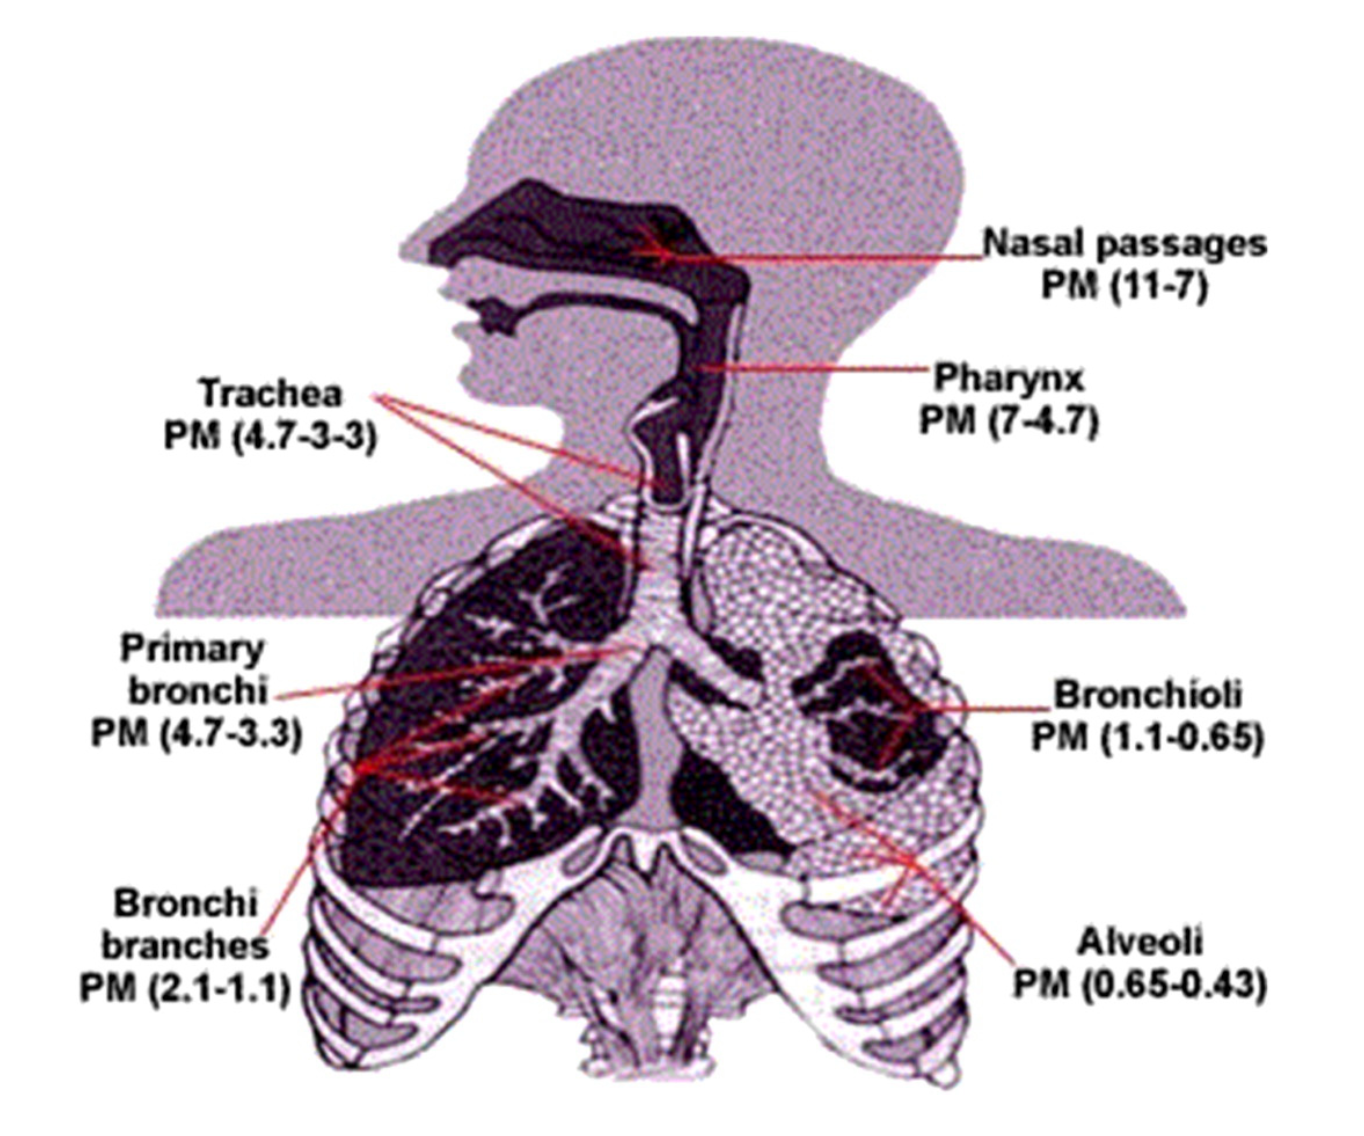
\includegraphics[scale=0.3]{images/Lungs.png}
    \caption{Potential deposition into the respiratory system of different size particles (Source: \cite{kim2015review})
}
    \label{fig:Lungs}
\end{figure}

Generally, PM enters the body through three major pathways:
\begin{enumerate}
    \item Inhalation: particles can enter through the respiratory tract. Depending on the sizing, as mentioned earlier, particles can penetrate deep into the lungs, reaching the alveolar region.
    \item Ingestion: PM can be present in contaminated food and beverage. Especially smaller particles penetrate deeper into the lungs where mucosal transport may not be as an effective removal mechanism.
    \item Dermal absorption: this is a passive process. Several factors can be considered, such as hair coverage, skin temperature and surface charge \cite{thompson2018airborne}.
\end{enumerate} 

Since inhalation is the predominant route of exposure \cite{broday2001growth}, the lungs are the primary affected organ.\\
People with chronic obstructive pulmonary disease (COPD), are the ones more sensitive to PM exposure \cite{sint2008ambient}. In particular, COPD is a progressive inflammatory condition of the lungs caused mainly by inhalation of noxious gases and PM \cite{ling2009particulate}.\\
The World Health Organization defined COPD as the third leading cause of death in 2019 \cite{whoChronicObstructive}.
Apart from inflammation, endotoxin effects, stimulation of capsaicin/irritation receptors autonomic nervous system activity and reactive oxygen species (ROS) production are observed. The latter process receives more attention \cite{li2008role}.\\
In particular, $\text{Fe}^{3+}$ can be reduced into $\text{Fe}^{2+}$ after entering the cells, which can then lead to the generation of ROS via the Fenton reaction and lipid peroxidation \cite{cory2019impact}. \\
Oxidative stress can also impact allergic inflammation, induce acute asthma exacerbations and production of antigen-inducted airway hyperactivity \cite{li2003particulate}.\\

The heart is another organ that can be directly affected by PM exposure. In particular, two different pathways have been shown: direct, especially for $\text{PM}_{2.5}$, which can traslocate directly into the bloodstream, and indirect, in which systemic inflammation poses a risk for atherosclerosis progression, increase of blood coagulability and leads to endothelial disfunction and myocardial ischemia \cite{du2016air}.
PM can also alter heart rate control by the autonomic nervous system through an increase in systolic blood pressure (Fig.\ref{fig:Heart}) \cite{fiordelisi2017mechanisms}. 

\begin{figure}[H]
\centering
    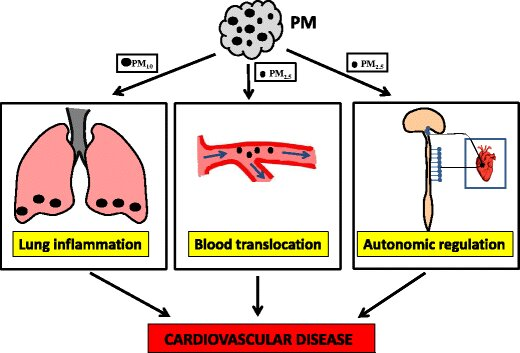
\includegraphics[scale=0.4]{images/Heart.jpg}
    \caption{Different mechanism in which PM can affect cardiovascular system (Source: \cite{fiordelisi2017mechanisms})
}
    \label{fig:Heart}
\end{figure}

Even the brain can be affected by airborne pollutant \cite{campbell2014human}, especially fine particulate matter containing heavy metals.\\
The brain is vulnerable to oxidative stress damage due to different factor: its high energy use which can generate lots of free radical, high metabolic demand and low level of endogenous scavengers, which means that is has less immune system that can neutralize free radical \cite{mohankumar2008particulate}. Ossidative stress can also influence some brain function, especially in children exposed to high levels of PM \cite{fagundes2015direct}.\\
PM can also contribute to the arise of neurodegeneration related disease such as Alzheimer’s disease (AD), Parkinson’s disease (PD) and dementia \cite{tsai2019fine}. \\
It was shown that in AD patients the levels of Fe, Cu and Zn are increased in the rims of senile plaques and Fe is high in the brain of PD patients \cite{campbell2005particulate}.\\
Inhaled PM can cross the air-to-blood tissue barrier of the lungs and reach the brain through two main pathways: directly entering via the olfactory sensory neurons or by crossing the blood-to-brain endothelial barrier \cite{hopkins2018repeated}.\\
Not only the size, but also the elements present in these particles can be problematic.
For example, the presence of Fe in PM can trigger the ferroptotic mechanism, leading to brain neuropathology \cite{cory2019impact}(Fig.\ref{fig:brain}).

\begin{figure}[H]
\centering
    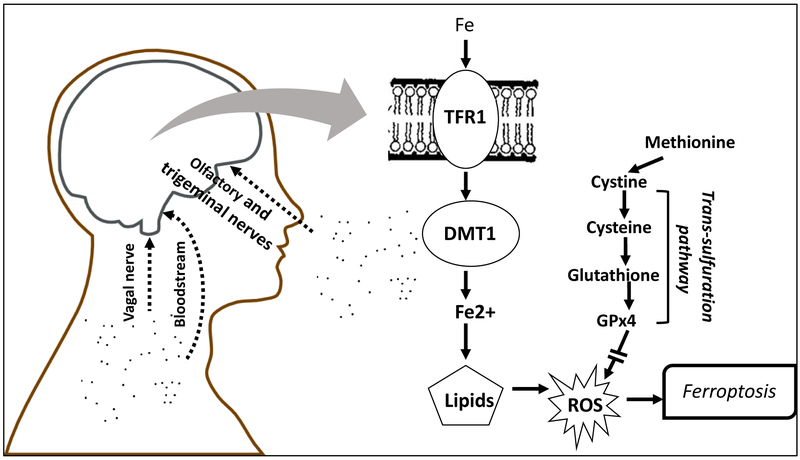
\includegraphics[scale=0.7]{images/brain.jpg}
    \caption{Diagram showing the possible pathway of ultrafine particles to the brain (Source: \cite{cory2019impact})
}
    \label{fig:brain}
\end{figure}

All this evidence proves that PM is an important factor to consider when addressing human health. Throughout their lives, people are continually exposed to PM, which can lead to a deterioration in quality of life. 
The focus on studying the PM characteristic can help understanding its nature and how it can interact with human body. \\
Considering now the area where most of the people live, it is inevitable to think about cities and their principal sources of PM. \\
Large urban areas are characterized by high pollutant emission rates due to the concentration of numerous human activities \cite{pandis2016urban}. \\
Traffic emissions are one of the major contributor to total PM \cite{pant2013estimation}, so focusing a significant portion of attention on particles emitted by vehicle circulation is warranted. \\

Generally, particles emitted from traffic are categorized into two main groups: exhaust emission from incomplete combustion and non-exhaust emission generated by wear and tear of vehicles and road surfaces \cite{grigoratos2015brake}(Fig.\ref{fig:emissions}).

\begin{figure}[H]
\centering
    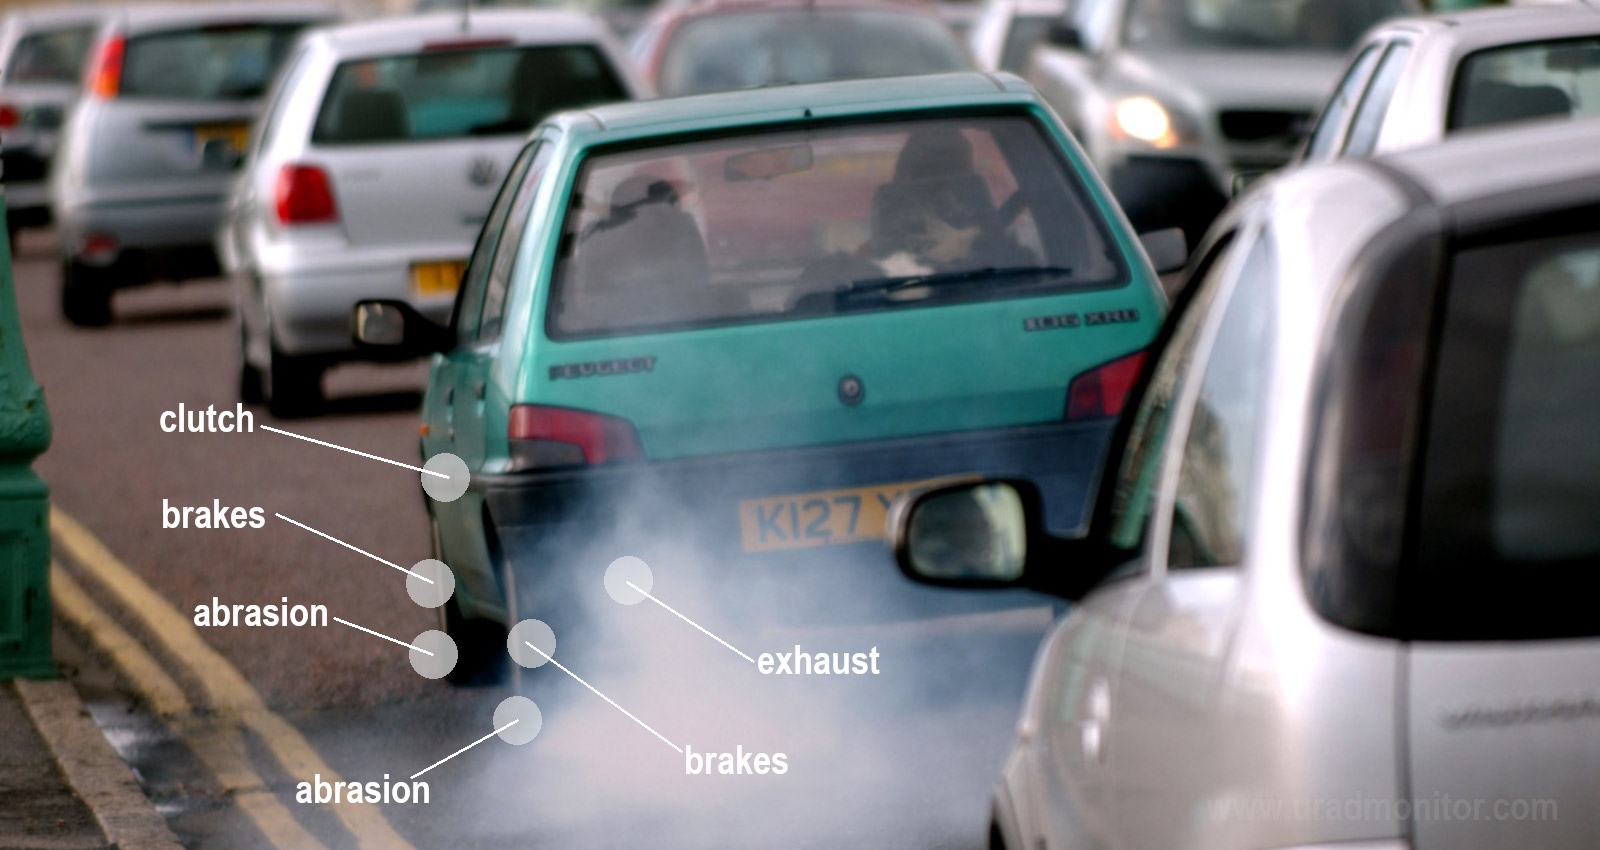
\includegraphics[scale=0.22]{images/emissions.jpg}
    \caption{Exhaust emissions resulting from the fuel combustion and non-exhausted emissions resulting from the wear and friction of varied surfaces (Source: Global Environmental Monitoring Network, 2023).
}
    \label{fig:emissions}
\end{figure}

It was proved that up to $70\%$ of brakes debris material becomes airborne as PM \cite{mulani2022review}.
To control the production of PM many limits exist, regulation such as the “Euro” emissions standards for exhaust vehicles emissions. However, limitation on non-exhaust PM emissions, primarily from tire and brake wear, are less stringent \cite{piscitello2021non}. 
Some regulations incentives hybrid or electric cars (EV) purchases to address this issue. \\
It goes without saying that the generation of exhaust emissions and greenhouse gases from vehicles within the urban environment will gradually decrease with the adoption of hybrid and electric cars. \\
These vehicles require significantly less maintenance than conventional gasoline or diesel-powered cars, particularly regarding the brake system. This reduced maintenance leads to fewer particles generated from wear and tear, making hybrid and electric cars more environmentally friendly in term of PM emissions. \\
However, it was proved that, for instance, electric cars do produce zero exhaust emissions and brake wear, but at the same time, due to their weight, they produce at the end the same amount of PM as internal combustion engine vehicles (ICEV) in terms of tyre wear, road wear and resuspension \cite{timmers2018non}. \\
This highlights the need for future regulations to address non-exhaust PM emissions alongside exhaust emissions for a more comprehensive approach to air quality management on both ICEV , hybrid cars and EV. \\
In this study, we focused on non-exhaust emission because they are less analyzed pollutants. Understanding these emissions is crucial to determine whether the ecological transition to electric and hybrid vehicles can effectively reduce human exposure to PM or if there are additional factors to take into consideration. \\


\section{Brakes}
The principal differences in car brake systems will be presented in this paragraph. \\
Conventional cars rely solely on hydraulic braking systems, in which the friction between the brake pad and rotor converts kinetic energy into heat. This process generates particles due to the high temperature and component wear and tear. \\
In contrast, hybrid and electric cars utilize a regenerative braking system. During braking, the wheels transfer kinetic energy to a generator, which converts a significant portion of this energy back into electricity to recharge the battery.\\ Additionally, the generator resistance helps in slowing down the vehicle. Friction brakes are only engaged in situations requiring more forceful braking.
Thanks to the regenerative braking system electric and hybrid vehicles release significantly less PM in the atmosphere compared to conventional cars. \\
However, it’s important to acknowledge that other factors can also impact the amount of the emitted non-exhaust PM. \\
One key factor is the vehicle mass. Heavier vehicles tend to generate more particles due to the increased wear and tear of brakes. Driving style also plays a role, frequent hard braking and acceleration can increase the amount of PM emitted. Moreover deceleration rates can influence PM generation, regenerative braking can help, but very rapid deceleration events may still required the use of traditional brakes \cite{hicks2023quantifying}. \\
It is not so easy though to affirm that hybrid and electric cars produce less PM, especially since the presence of a battery can significantly increase their weight. \\
Another factor to take into consideration is the brake type. Generally, two types of brakes are used for cars (Fig.\ref{fig:brakes}):

\begin{figure}[H]
\centering
    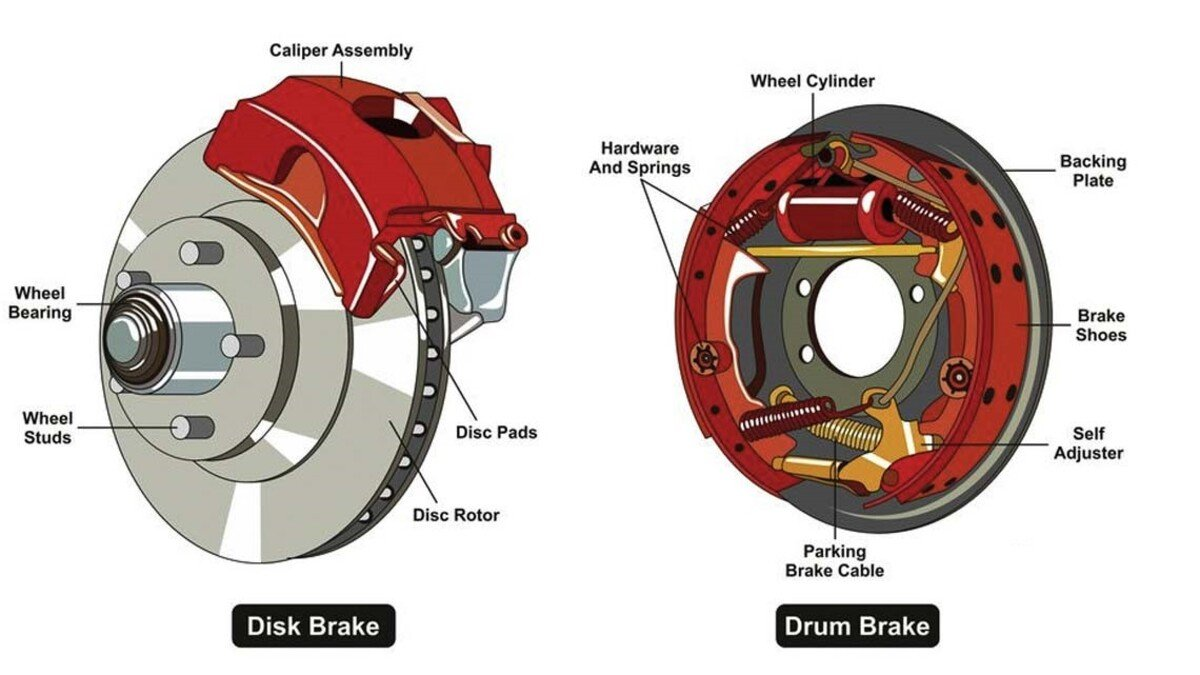
\includegraphics[scale=0.20]{images/brakes.jpg}
    \caption{Schematic representation of the two type of brakes: disc and drum (Source: Sahaj Palla, 2021).
}
    \label{fig:brakes}
\end{figure}


\begin{itemize}
    \item Disc brake, with a disc that turns with the wheel and a caliper. During braking, the caliper clamps down on the disc and the friction actions slows the wheels.
    \item Drum brake, with a hollow drum that turns with the wheel and two shoes. In this case, during braking the wheel cylinder pushes the shoes against the drum.  
\end{itemize}
Typically, modern vehicles have disc brakes on both the front and rear axles. Disc brakes provide superior stopping power and heat dissipation compared to drum brakes, which were commonly used on the rear axels of older vehicles. In even older vehicles, drum brakes might have been present on all four wheels. \\

During braking, a significant portion of the vehicle weight transfers to the front wheels. Front brakes handle about $70\%$ of a car’s total braking PM \cite{grigoratos2015brake}.
The composition of brakes pads is a critical factor, especially when considered in terms of the impact on human health. Typically, the formulation of brakes contains various heavy metals that can be harmful if inhaled or ingested in excessive amounts.
These heavy metals are present because brake pads are composed of a complex mixture of materials, each playing a specific role, such as:
\begin{itemize}
    \item Reinforcing fibers: provide structural integrity and stability. They are usually made of copper fibers, steel, brass, glass and carbon fibers.
    \item Fillers: improving thermal proprieties, noise dampening and reduce manufacturing costs. They are made of barite, potassium titanite, magnesium and chromium oxides.
    \item Abrasives: increasing friction and keep the breaks steady. They are made of zircon, quartz, aluminium and iron oxides.
    \item Lubrificants: minimize friction between the pad and the rotor. They are usually made of graphite.
\end{itemize}

Particles produced by braking often contain toxic metals like Fe, Ni, Cr, and Cu, which can generate harmful ROS. Additionally, research suggests that a higher proportion of Al in $\text{PM}_{2.5}$ can increase mortality rates \cite{kelly2012size}. \\
However, the specific composition varies significantly between manufactures and the materials and proportions vary depending on the characteristic and required performance. \\
Considering brake pad dust as a non-exhaust emission potentially harmful to humans, we can understand the danger it poses not only as a foreign body, but also due to the individual elements themselves. \\
Generally, Fe is considered the primary element in non-exhausted emissions because disc brakes are typically made of grey cast iron \cite{zemlik2022case}. \\
The wear during braking is severe, with the consequence of forming a large number of particles between the contact surfaces of friction pairs, this part is called the third body \cite{yao2023influence}. \\

Research has shown that magnetite is the primary component of friction films formed during braking. Its presence in the third body is attributed to the tribochemical oxidation of steel and iron as well as the transfer of pre-existing magnetite from the brake pad formulation \cite{yao2023influence}. \\
Furthermore, magnetite association with other elements such as Al, Ti, Ni and Pt might further elevate its toxicity \cite{ripley2024within}.
Additional research indicates that around 400°C, both magnetite and maghemite synthesized on the friction layer. As temperature reach 600°C, hematite may also be present \cite{hagino2023iron}.
Due to their formation during braking, these minerals can become dispersed in the air and inhaled by humans. This raise concerns about their potential accumulation in various organs. \\
Another concern is graphite, a common component in brake pads for lubrification and reinforcement.
Studies indicate that graphite can induce cell death (apoptosis) in lung cells \cite{zendehdel2023human}. \\ 
The combined presence of graphite with metal particles, known to trigger inflammatory response, could potentially exacerbate these effects. \\
Cu, for instance, is a common material used in brakes due to its ability to mitigate thermal fade and conductivity \cite{lee2013friction} \\
While essential for brain function, can become detrimental at high levels. Its strong redox potential can lead to oxidative stress and contribute to brain disease \cite{an2022role}, but can be also harmful to aquatic organisms \cite{lee2013friction}. \\

Nowadays, researchers are increasingly focused on substituting conventional materials, used in brakes formulations, with more environmentally friendly alternatives. For instance, significant efforts are being directed towards the use of natural fibers as reinforcement in composites \cite{hemanth2023eco} and the development of eco-friendly coating solutions to enhance the protection of automotive grey cast iron brake disks \cite{wank2023environmentally}. \\
These advancements not only aim to reduce the environmental impact but also to improve the performance and durability of automotive components.



\section{Experiment}

This study aims to characterize brake dust from different vehicles types using various techniques.
The characterization will encompass both chemical and morphology (shape and size) of the powders. \\
This analysis aims to identify the primary constituents of friction particles generated during braking and investigate potential variations between different vehicle types. \\
A dissolution test will then be conducted to investigate how these brake dust particles might interact with simulated biofluids, specifically a brain-like environment. \\
The selection of car types aimed to achieve a variety of vehicles classes, thereby considering the key parameters that influence brake dust generation. This variation included differences in engine type and weight. \\
In particular, 5 cars were taken in consideration: 
\begin{itemize}
    \item 3 conventional cars, Fiat Panda 169 (800kg), Fiat 500L (1250 kg), Fiat 500X (1300 kg).
    \item 1 liquefied petroleum gas car (LPG), Ypsilon Lancia (1040 kg). \\
    \item 1 hybrid car, Corolla Toyota (1400 kg).
\end{itemize}

For each car the powders were collected on the surface of the caliper for the disc brakes and from the shoes for the drum ones. Both anteriors and posteriors wheels were sampled. \\
EV were not included in this study due to the difficulty in obtaining a representative sample, as they are less readily available.

  










\afterpage{\blankpage}
\chapter{Materials and Methods}

In order to collect brake dust samples, the front wheels of the vehicle were first removed. Brake dust was then carefully collected from the brake calipers and discs of both of the front wheels using a clean brush. The collected dust from each front wheel was then transferred into a labeled test tube. This process was repeated for the rear wheels, ensuring that the brake dust from each rear wheel was collected and stored in separate labeled test tubes.\\
This means that each test tube contained brake dust from 2 wheels at a time. \\
As a result, a total of 10 samples, 5 from the front and 5 from the rear, were collected and were given the following names: Panda Ant and Post, 500X Ant and Post, 500L Ant and Post, Ypsilon Ant and Post, Corolla Ant and Post.

\section{Powder X-Ray Diffraction (PXRD)}

Initially, the collected powders were analyzed using Powder X-Ray Diffraction (PXRD) with a PXRD MINIFLEX 600 diffractometer to better understand the main mineral phases present. \\
Each sample was hand-ground using an agate mortar and then placed on a glass PXRD sample holder. \\
The only sample that was not included is the Corolla Post, due to the insufficient amount of powder for the needs of the measurement instrument.\\
The analyses were performed in a range between 3 and 80° $2\Theta$ with 0.020° step and 1.0 deg/min speed and then each diffractogram was elaborated using the “EVA” software.

\section{Scanning Electron Microscopy with Energy Dispersive X-ray Spectroscopy (SEM-EDX)}

The second part of the characterization was performed by using the Scanning Electron Microscope (SEM VEGA TESCAN) to obtain semi-quantitative standardless chemical information and collect morphometric data on the particles. \\
The samples were prepared by positioning the SEM Al-stubs close to the sample containing tube and the brake powder was dry dispersed onto the stubs by blowing a gentle air flux within the tube to promote homogeneous dispersion of particles. The stubs were finally C-coated for the analysis. \\
The samples were observed in SEM-SE and SEM-BSE modes to obtain reliable information on both their morphology and chemistry. \\
For the chemical and dimensional analyses, the SEM was set at a voltage of 30 keV, with z parameter and working distance at 15 mm. For the morphological analyses, the working distance was set at 5 mm. \\
The most representative particles of the sample were chosen for the morphological analyses.\\
The EDXS spectra were collected from 10 spots in each of the 10 analyzed areas of the 10 samples, resulting in 100 spectra per sample and a total of 1000 spectra.
These analyses were useful to understand the main elements present in the sample and to compare them with the mineral phases found in the PXRD analyses. \\

From the same SEM-BSE images used for the chemical analyses, dimensional analyses were also performed using the software “ImageJ”. \\
By making the image binary, the software can identify the particles present and calculate their diameters. \\
For the diameter measurement, the software uses the “Feret” diameter, which is defined as the statistical diameter representing the mean value of distances between pairs of parallel tangents to a projected outline of particles \cite{wang}. \\
It is generally used for analysis of particles to apply the projection of a 3D object on a 2D plane. \\
The calculated measurements were then used to generate a size distribution histogram employing the matplotlib Python library. The analysis focused on particles with diameters smaller than 15 µm due to their potential health risk \cite{epaHealthEnvironmental}. \\
For the size distribution histogram, the diameter range on the x-axis was set from 0 to 15 µm to focus on particles cited before. The number of bins in the histogram was chosen arbitrarily as 20 for better visualization of the data. \\
The y-axis represents the absolute frequency , which is the number of particles observed within each diameter range. \\
It is important to note that the number of particles in each sample might vary. This is because the SEM-BSE images were captured randomly and the samples themselves likely have inherent heterogeneity. \\

The chemical information obtain from SEM-EDX analysis was also analyzed using the matplotlib Python library. The analysis focused on detecting the presence of heavy metals within the samples. \\
Each spectra (100 for each sample) was examined to count the number of times specific heavy metal was detected. \\
The result was a grouped bar chart for each car, visualizing the presence of the main heavy metals identified with SEM-EDX. This allowed for a sample-by-sample comparison of the heavy metals content. \\

\section{Dissolution Test and Inductively Coupled Plasma (ICP)}

The third part of the experiment was the dissolution test using simulated biofluid. This technique is used to test the possible reaction of the particles present in the samples within a biological environment. The biofluid used in this experiment was a saline solution ($0.9\%$ NaCl) \cite{innes2021simulated} with a pH of 7.4, mimicking pH of blood plasma \cite{atherton2009acid}. \\
The samples used for the test were from the 3 car types: Panda Ant (combustion engine), Ypsilon Ant (LPG car) and Corolla Ant (hybrid car). The decision to use only front brake powders was based on the factor that they typically generate more particles compared to rear brakes and contribute more significantly to overall brake powders emissions due to their role in deceleration. \\
The dissolution test was conducted in an orbital shaker incubator at a temperature of 39 °C to simulate physiological conditions \cite{rzechorzek2022daily}. \\
For each sample, 2 mg of brake powders were used for each sample and dissolved in 2 ml of saline solution \cite{zhang2022hpmc}, the decision to use 2 mg of powders was made to ensure consistency across the samples, mainly due to the lower amount of material available for the sample Corolla Ant \\
The test was performed at six different time points: $\text{t}_{0.5}$, $\text{t}_{1}$, $\text{t}_{12}$, $\text{t}_{24}$, $\text{t}_{48}$ and $\text{t}_{168}$. At each time-point, the sample solution was removed and placed in another tube for ICP analysis. This analysis focused on the amount of Fe released into the liquid over time.

\section{Atomic Resolution Scanning Transmission Electron Microscopy (AR-STEM)}

The fourth part of the experiment was the characterization using Atomic Resolution Scanning Transmission Electron Microscopy (AR STEM) Jeol, ARM 200 CF. \\
STEM analysis was performed on both pre-interaction and post-interaction samples from Panda Ant, Ypsilon Ant and Corolla Ant used for the dissolution test.\\
Pre-interaction samples were rinsed with distilled water to remove contaminants and then placed in an ultrasonication bath for 10 minutes at 40°C to dislodge weakly attached particles. After this, 8 drops of sample was deposited onto a TEM grid for analysis. \\
For the post-interaction samples, only the solution from the $\text{t}_{168}$ time point (longest interaction time) was used for STEM analysis. This solution was first centrifuged for 5 minutes at 5000 RPM to separate the remaining brake particles from the liquid phase. The resulting saline solution was collected for ICP analysis. Following this, the particles were subjected to an ultrasonic bath for 10 minutes at 40°C. Finally, 8 drops of the prepared sample suspension was deposited onto a TEM grid for analysis, following the same procedure as the pre-interaction samples. \\
For TEM analyses, a voltage of 80 kV was used. Both low-resolution and high-resolution images were captured for each sample, allowing for initial observation and detailed examination of specific features within the particles. EDXS analysis was then performed on 10 particles from each sample to identify the main elements present. The goal was to compare these findings with the results obtained from PXRD and SEM-EDX analyses, looking for correlations between the different techniques.\\ Additionally, an elemental map was acquired for the most representative particles, visually depicting the distribution of the most abundant elements within that particulate particle.\\
At the end, Dual Electron Energy Loss Spectroscopy (Dual EELS) was performed on 5 particles per sample to investigate the valence state of Fe.
\chapter{Results}

This chapter is a comprehensive collection of all the outcomes originating from the analyses presented in the previous one.\\
For the SEM-EDX analysis, it will be presented the results before and after the intraction with the biofluid.\\
More details and interpretations will be discussed in the Discussion chapter.

\section{PXRD}

The PXRD spectra of all powders revealed complex compositions with various mineral phases. Many peaks overlap, but some were more visible and interpretable than others. \\
For this study as many phases as possible were considered, but in the results only the main phases (the ones with higher peaks) will be taken into consideration. \\
The full width half maximum of some peaks reveals also the presence of some amorphous phases. \\

\textbf{Panda Ant} \\
The spectrum obtained (Fig.\ref{fig:Panda_Ant_PXRD}) showed narrow and high peaks that helped with the identification of some mineral phases:

\setlist{nolistsep}
\begin{enumerate}[noitemsep]
    \item Magnetite (JCPDS code: 00-019-0629)
    \item Hematite (JCPDS code: 00-001-1053)
    \item Quartz (JCPDS code: 00-001-0649)
    \item Graphite (JCPDS code: 00-002-0456)
    \item Aluminium Iron Silicon (JCPDS code: 00-045-1205)
    \item Donathite (JCPDS code: 00-022-0349)
\end{enumerate}

\begin{figure}[H]
\centering
    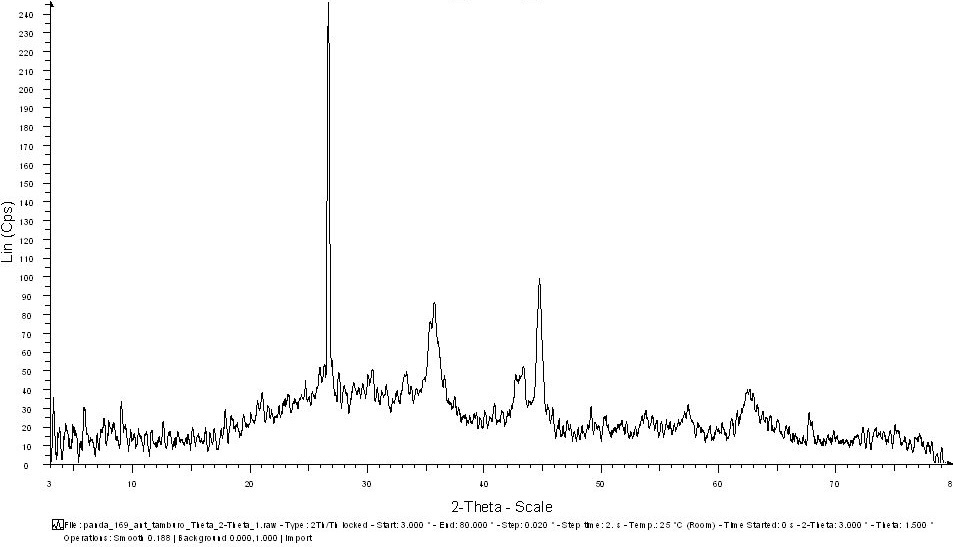
\includegraphics[scale=0.46]{images/panda_169_ant_edit.jpg}
    \caption{PXRD spectrum of Panda Ant sample.}
    \label{fig:Panda_Ant_PXRD}
\end{figure} 

\textbf{Panda Post} \\
The spectrum (Fig.\ref{fig:Panda_Post_PXRD}), in this case, showed some different peaks, but more background. \\
The mineral phases identified were the following:

\setlist{nolistsep}
\begin{enumerate}[noitemsep]
    \item Quartz (JCPDS code: 00-033-1161)
    \item Hematite (JCPDS code: 00-001-1053)
    \item Graphite (JCPDS code: 00-002-0456)
    \item Aluminium Iron Silicon (JCPDS code: 00-045-1205)
    \item Iron (JCPDS code: 00-003-1050)
    \item Magnetite (JCPDS code: 00-019-0629)
    \item Maghemite (JCPDS code: 00-013-0458)
\end{enumerate}

\begin{figure}[H]
\centering
    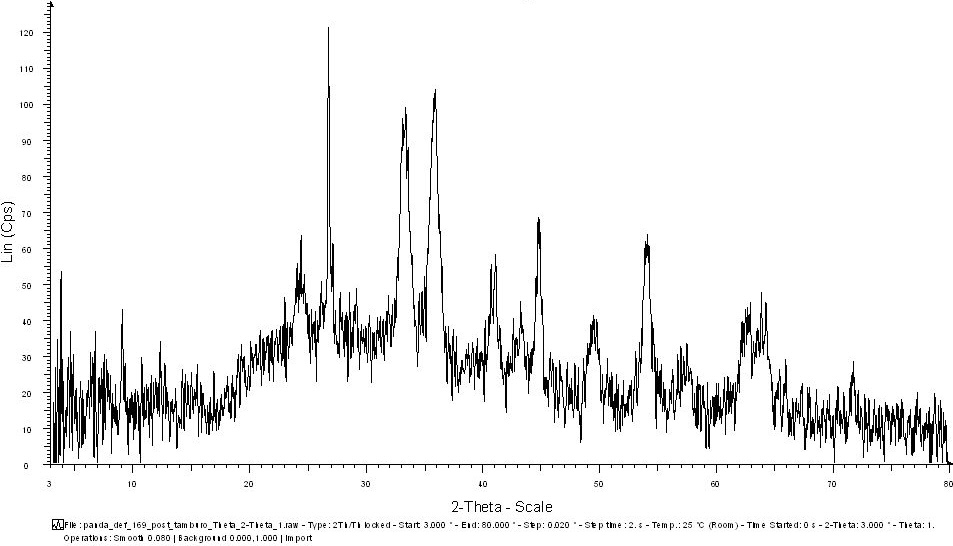
\includegraphics[scale=0.46]{images/panda_169_post_edit.jpg}
    \caption{PXRD spectrum of Panda Post sample.}
    \label{fig:Panda_Post_PXRD}
\end{figure} 

\pagebreak

\textbf{500X Ant} \\
The spectrum (Fig.\ref{fig:500X_Ant_PXRD}) showed some major peaks attributed to:

\setlist{nolistsep}
\begin{enumerate}[noitemsep]
   \item Magnetite (JCPDS code: 00-019-0629)
    \item Maghemite (JCPDS code: 00-004-0755)
    \item Copper Iron Manganese Oxide (JCPDS code: 00-020-0358)
    \item Hematite (JCPDS code: 00-033-0664)
    \item Graphite (JCPDS code:00-002-0456)
    \item Aluminium Iron Silicon (JCPDS code: 00-045-1205)
    \item Goethite (JCPDS code: 00-003-0249)
\end{enumerate}

\begin{figure}[H]
\centering
    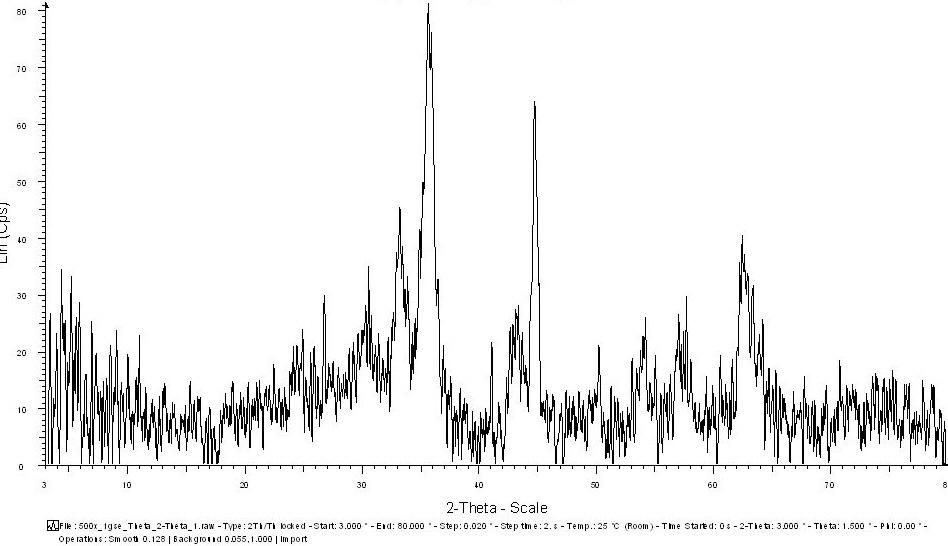
\includegraphics[scale=0.46]{images/500X_1gse_disco_ant_edit.jpg}
    \caption{PXRD spectrum of 500X Ant sample.}
    \label{fig:500X_Ant_PXRD}
\end{figure} 

\textbf{500X Post} \\
The spectrum (Fig.\ref{fig:500X_Post_PXRD}) showed some major peaks attributed to:

\setlist{nolistsep}
\begin{enumerate}[noitemsep]
    \item Magnetite (JCPDS code: 00-001-1111)
    \item Quartz (JCPDS code: 00-033-1161)
    \item Coesite (JCPDS code: 00-014-0654) or Iron Phosphate (JCPDS code: 00-0-14-0147)
    \item Manganese Iron Oxide (JCPDS code: 00-024-0507)
    \item Aluminium Copper Manganese (JCPDS: 00-025-1122) or Sodium Aluminium Oxide (JCPDS: 00-020-1073)
\end{enumerate}

\begin{figure}[H]
\centering
    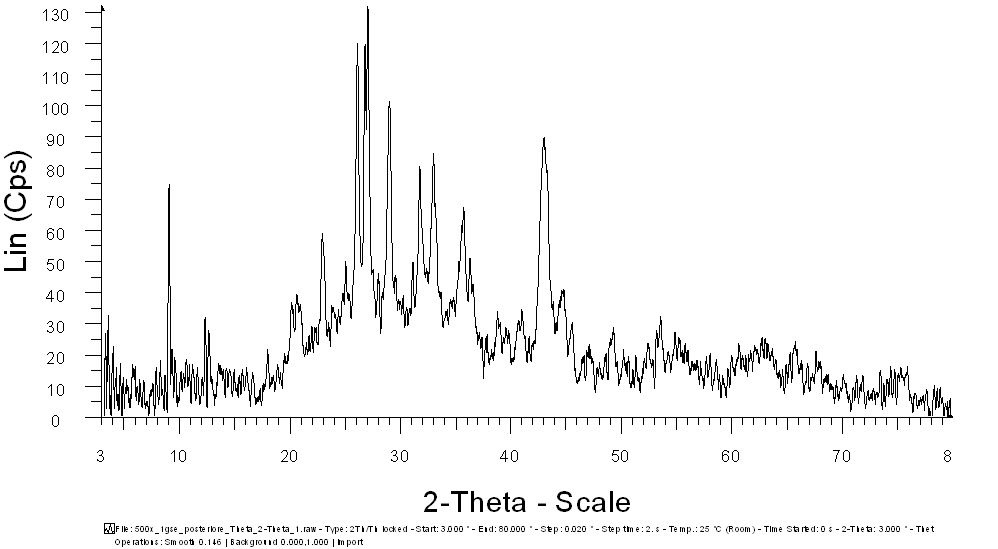
\includegraphics[scale=0.46]{images/500x_post.jpg}
    \caption{PXRD spectrum of 500X Post sample.}
    \label{fig:500X_Post_PXRD}
\end{figure} 

\textbf{500L Ant} \\
The spectrum (Fig.\ref{fig:500L_Ant_PXRD}) showed some major peaks attributed to:

\setlist{nolistsep}
\begin{enumerate}[noitemsep]
    \item Magnetite (JCPDS code: 00-019-0629)
    \item Hematite (JCPDS code: 00-033-0664)
    \item Maghemite (JCPDS code: 00-004-0755)
    \item Allophane (JCPDS code: 00-038-0449)
    \item Graphite (JCPDS code: 00-002-0456)
    \item Goethite (JCPDS code: 00-002-0281)
\end{enumerate}

\begin{figure}[H]
\centering
    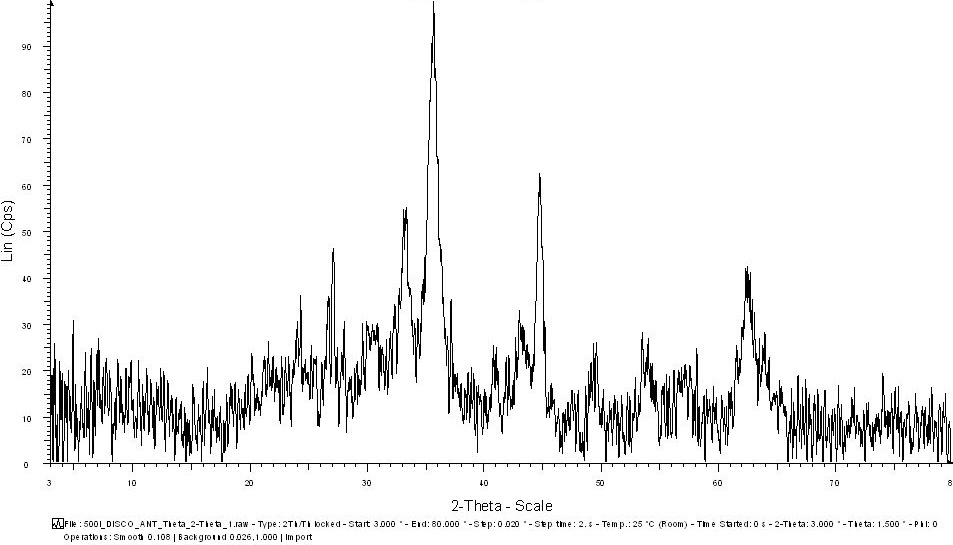
\includegraphics[scale=0.46]{images/500L_DISCO_ANT_edit.jpg}
    \caption{PXRD spectrum of 500L Ant sample.}
    \label{fig:500L_Ant_PXRD}
\end{figure} 

\textbf{500L Post} \\
The spectrum (Fig.\ref{fig:500L_Post_PXRD}) showed some major peaks attributed to:

\setlist{nolistsep}
\begin{enumerate}[noitemsep]
    \item Magnetite (JCPDS code: 00-025-1376)
    \item Hematite (JCPDS code: 00-024-0072)
    \item Maghemite (JCPDS code: 00-004-0755)
    \item Quartz (JCPDS code: 00-001-0649)
    \item Aluminium Iron Silicon (JCPDS: 00-045-1206)
\end{enumerate}

\begin{figure}[H]
\centering
    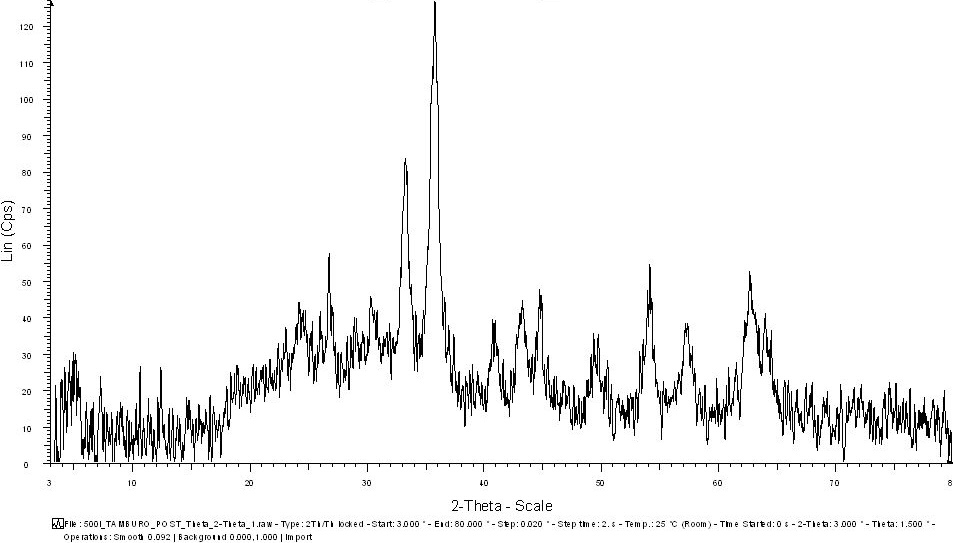
\includegraphics[scale=0.46]{images/500L_tamburo_post_edit.jpg}
    \caption{PXRD spectrum of 500L Post sample.}
    \label{fig:500L_Post_PXRD}
\end{figure} 

\textbf{Ypsilon Ant} \\
The spectrum (Fig.\ref{fig:Ypsilon_Ant_PXRD}) showed some major peaks attributed to:

\setlist{nolistsep}
\begin{enumerate}[noitemsep]
    \item Magnetite (JCPDS code: 00-019-0629)
    \item Hematite (JCPDS code: 00-033-0664)
    \item Maghemite (JCPDS code: 00-004-0755)
    \item Iron (JCPDS code: 00-103-1050)
\end{enumerate}

\begin{figure}[H]
\centering
    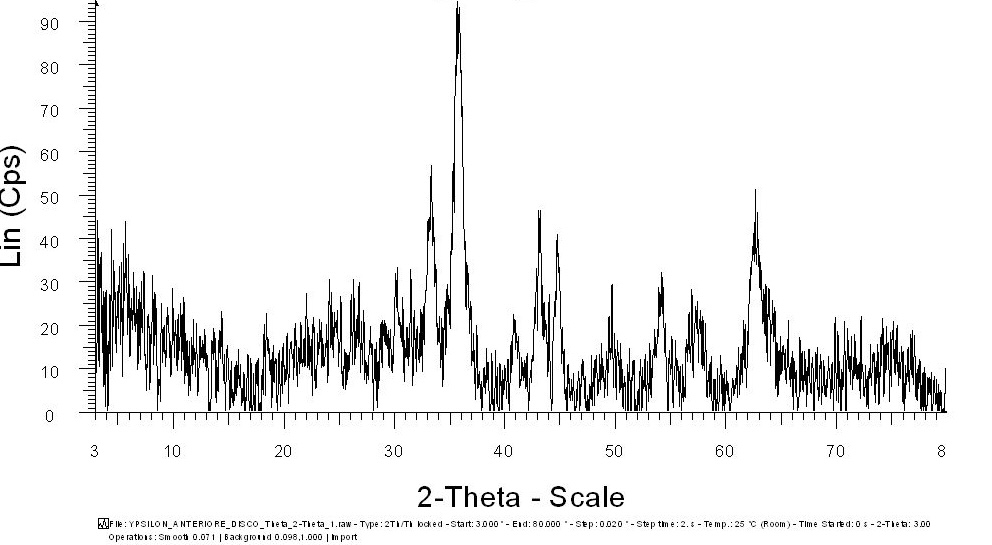
\includegraphics[scale=0.46]{images/YPSILON_ANT_DISCO.jpg}
    \caption{PXRD spectrum of Ypsilon Ant sample.}
    \label{fig:Ypsilon_Ant_PXRD}
\end{figure} 

\textbf{Ypsilon Post} \\
The spectrum (Fig.\ref{fig:Ypsilon_Ant_PXRD}) showed some major peaks attributed to:

\setlist{nolistsep}
\begin{enumerate}[noitemsep]
    \item Magnetite (JCPDS code: 00-025-1376)
    \item Hematite (JCPDS code: 00-033-0664)
    \item Maghemite (JCPDS code: 00-013-0458)
    \item Quartz (JCPDS code: 00-005-0490)
    \item Iron (JCPDS code: 00-006-0696)
\end{enumerate}

\begin{figure}[H]
\centering
    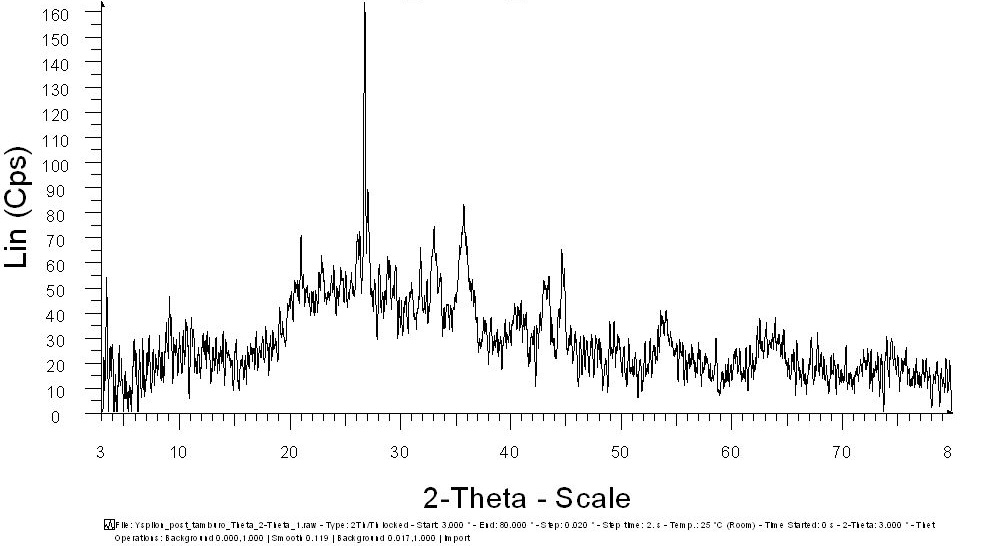
\includegraphics[scale=0.46]{images/YPSILON_POST_TAMBURO.jpg}
    \caption{PXRD spectrum of Ypsilon Post sample.}
    \label{fig:Ypsilon_Post_PXRD}
\end{figure} 

\textbf{Corolla Ant} \\
The spectrum (Fig.\ref{fig:Ypsilon_Ant_PXRD}) showed some major peaks attributed to:

\setlist{nolistsep}
\begin{enumerate}[noitemsep]
    \item Magnetite (JCPDS code: 00-025-1402)
    \item Aluminium Iron Silicon (JCPDS code: 00-045-1205)
    \item Maghemite (JCPDS code: 00-025-1402)
    \item Quartz (JCPDS code: 00-005-0490)
    \item Copper Magnesium Tin (JCPDS code: 00-034-1092) or Copper Tin (JCPDS code: 00-031-0485)
\end{enumerate}

\begin{figure}[H]
\centering
    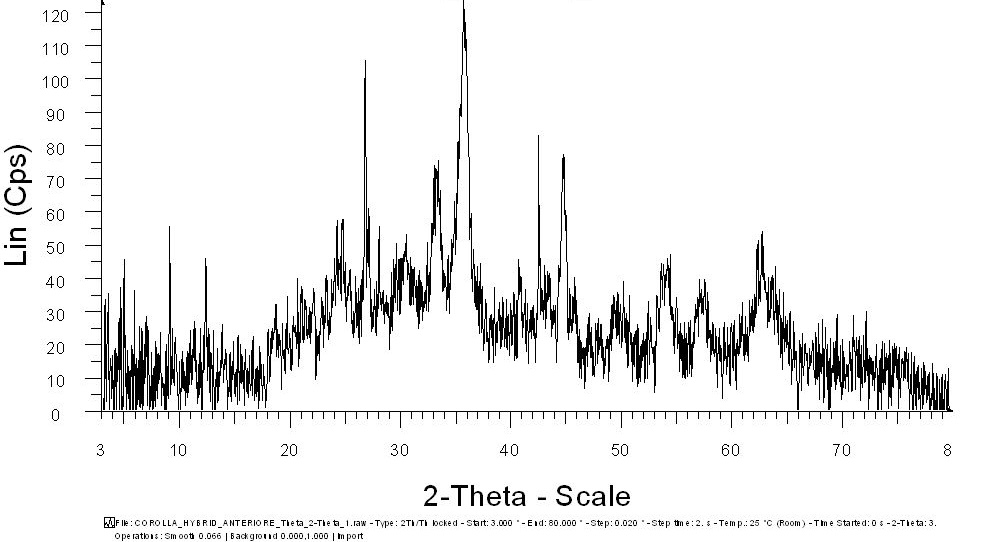
\includegraphics[scale=0.46]{images/Corolla_Hybrid_Ant.jpg}
    \caption{PXRD spectrum of Corolla Ant sample.}
    \label{fig:Corolla_Ant_PXRD}
\end{figure} 
\pagebreak

\section{SEM-EDX Before Interaction}

\subsection{Dimensional Analyses}

For each sample a histogram was created using the "Feret" values obtained with "ImageJ".\\
On the x-axis, the particle diameters corresponding to the "Feret" values were plotted, and on the y-axis, the number of particles with the corresponding diameters was reported. \\
Two red lines were added to each histogram to delineate the diameter values of interest, specifically those under 10 µm, between 10 µm and 2.5 µm, and below 2.5 µm.\\
The resulting histograms were the following:

\begin{figure}[H]
\centering
\begin{subfigure}{.5\textwidth}
  \centering
  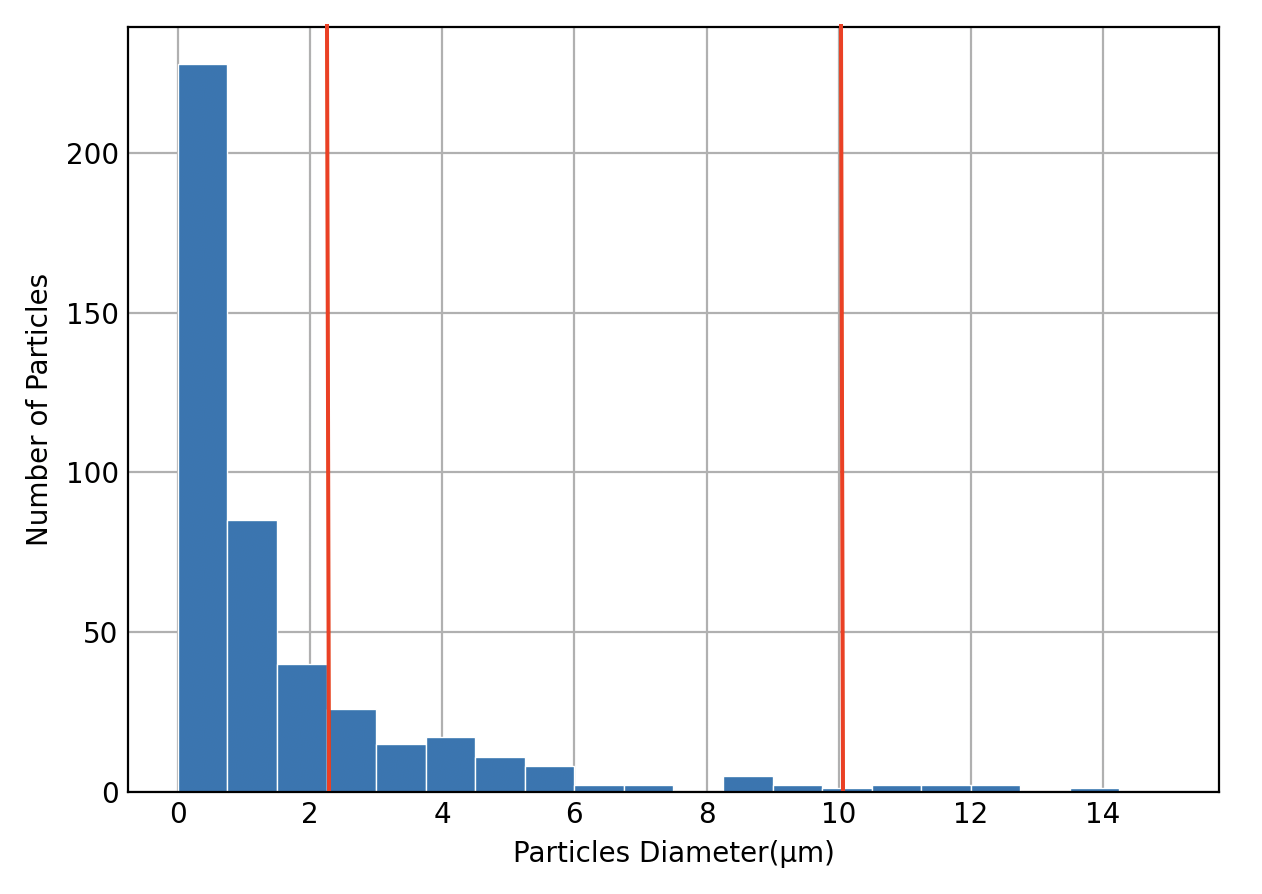
\includegraphics[width=1\linewidth]{images/Panda_Ant_D.png}
  \caption{Panda Ant}
  \label{fig:pandaant}
\end{subfigure}%
\begin{subfigure}{.5\textwidth}
  \centering
  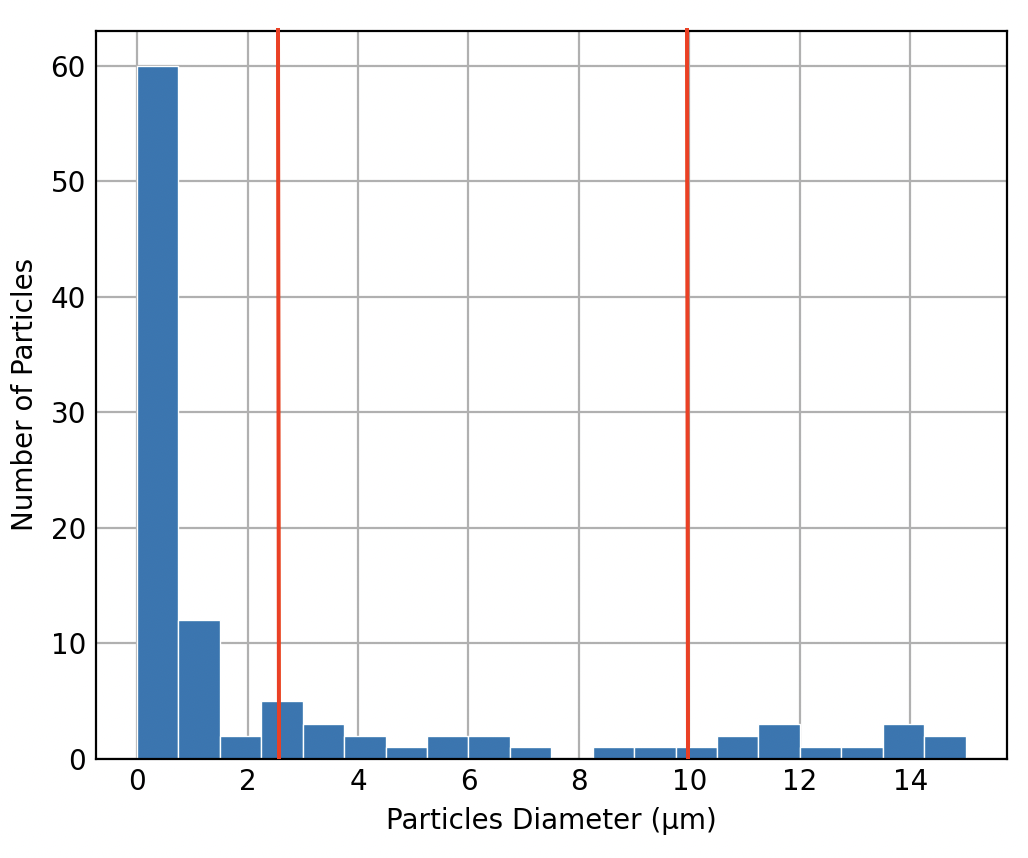
\includegraphics[width=0.85\linewidth]{images/Panda_Post_D.png}
  \caption{Panda Post}
  \label{fig:pandapost}
\end{subfigure}
\caption{Diameter distribution histograms of Panda sample}
\label{fig:1}
\end{figure}

\begin{figure}[H]
\centering
\begin{subfigure}{.5\textwidth}
  \centering
  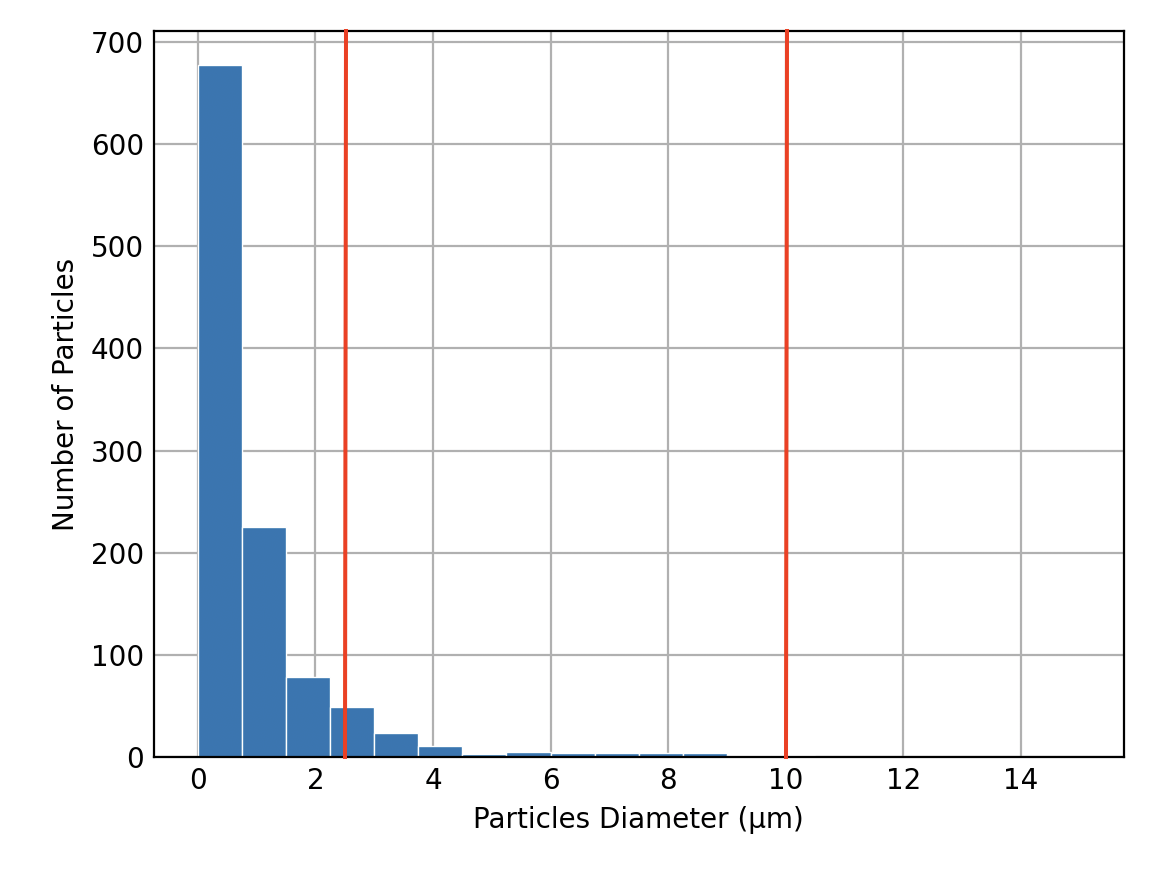
\includegraphics[width=1\linewidth]{images/500X_ant_dis.png}
  \caption{500X Ant}
  \label{fig:500xant}
\end{subfigure}%
\begin{subfigure}{.5\textwidth}
  \centering
  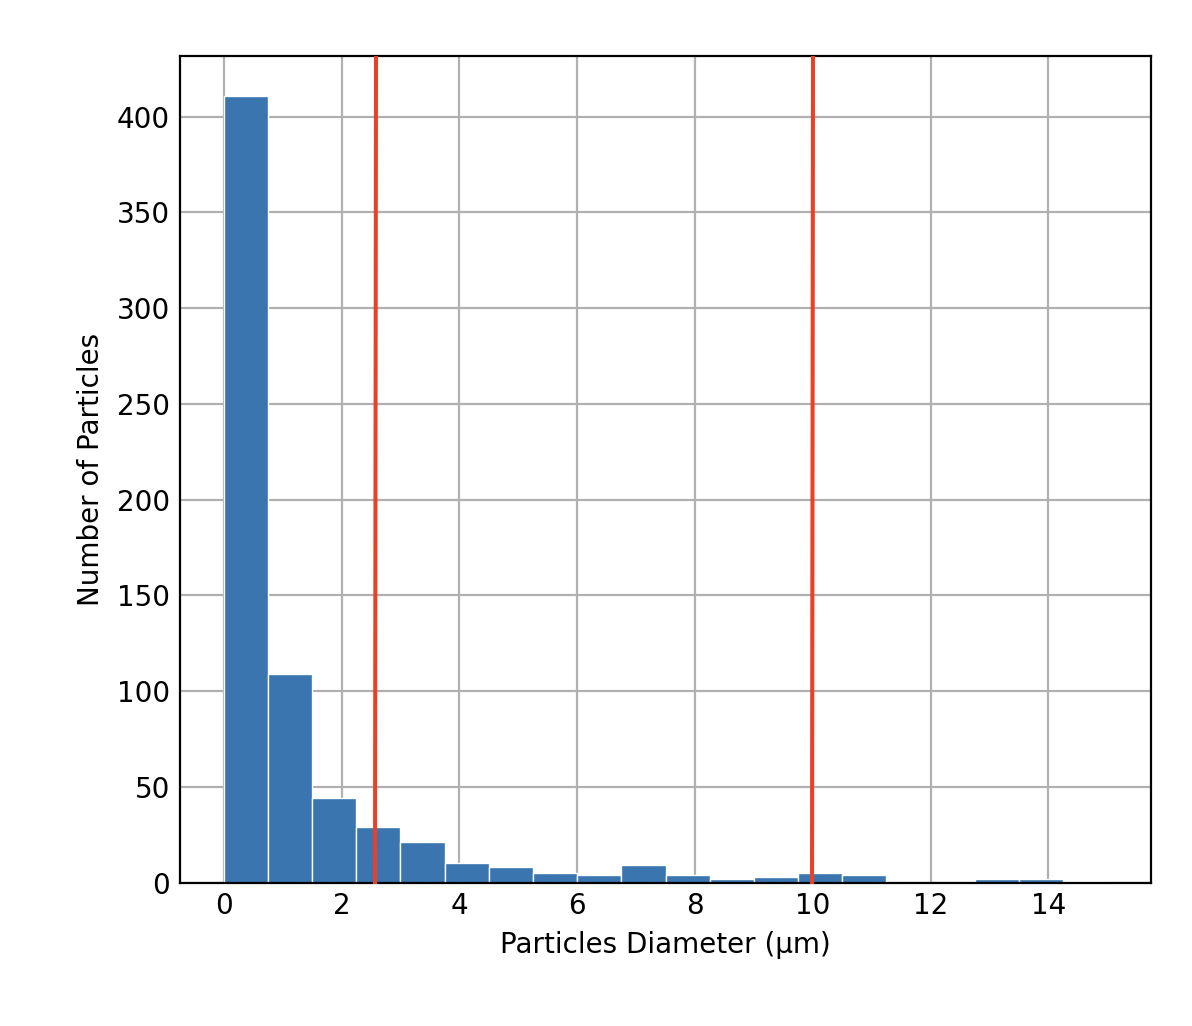
\includegraphics[width=0.9\linewidth]{images/500X_post_dis.png}
  \caption{500X Post}
  \label{fig:500xpost}
\end{subfigure}
\caption{Diameter distribution histograms of 500X sample}
\label{fig:2}
\end{figure}

\begin{figure}[H]
\centering
\begin{subfigure}{.5\textwidth}
  \centering
  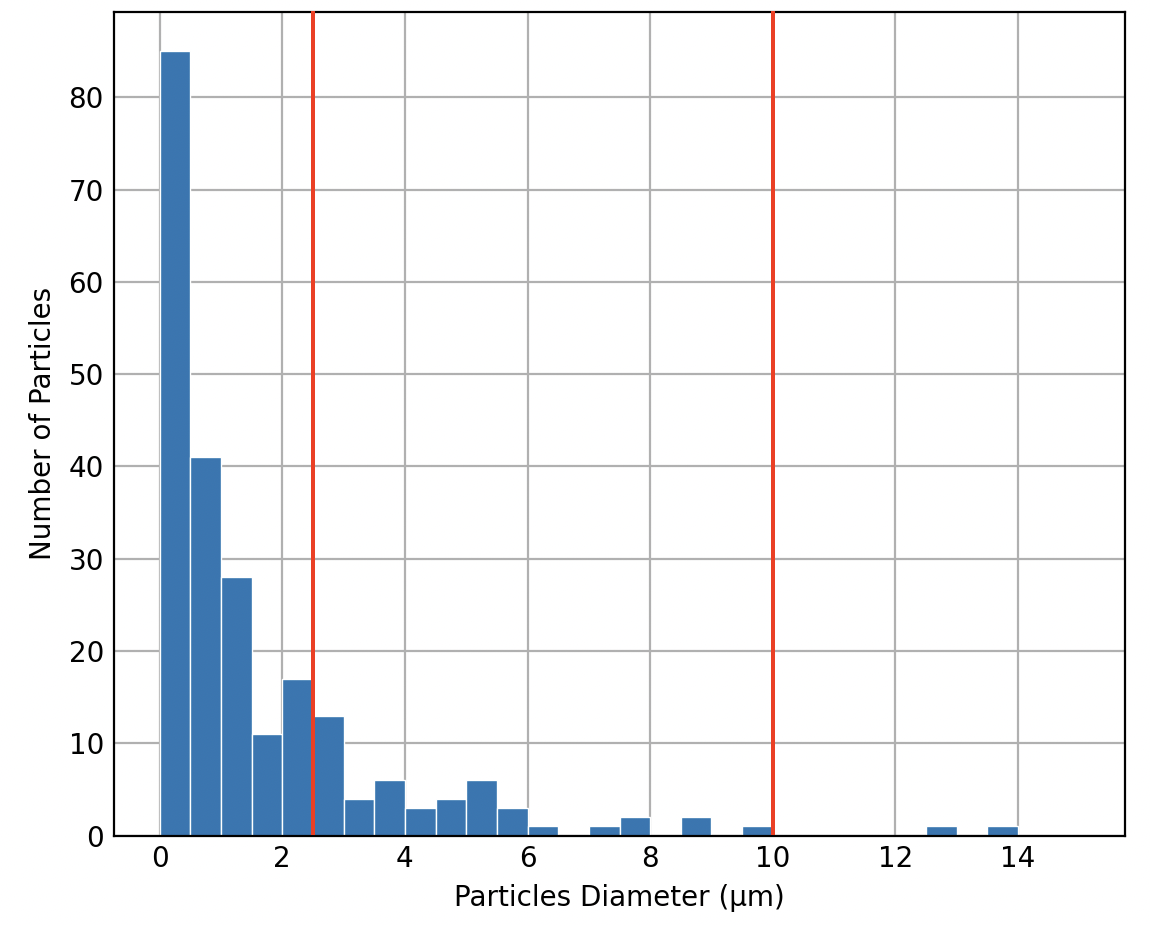
\includegraphics[width=0.85\linewidth]{images/500L_Ant_D.png}
  \caption{500L Ant}
  \label{fig:500lant}
\end{subfigure}%
\begin{subfigure}{.5\textwidth}
  \centering
  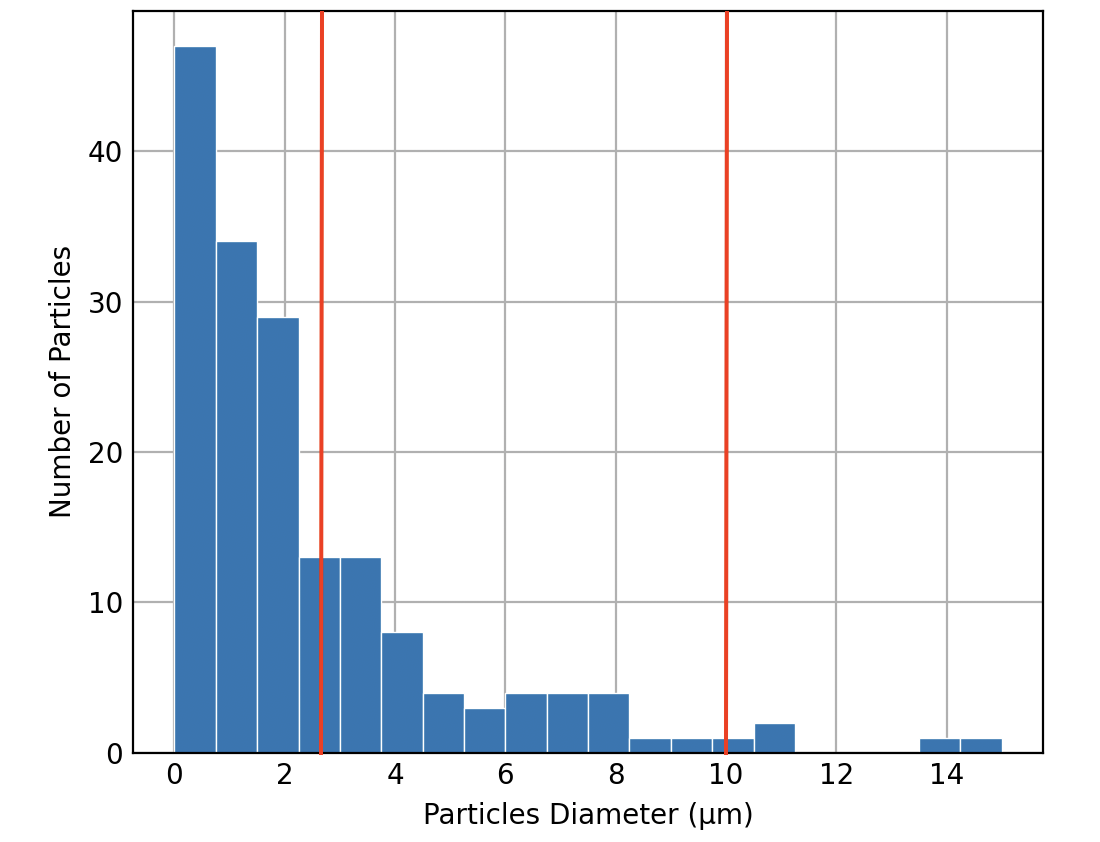
\includegraphics[width=0.9\linewidth]{images/500L_Post_D.png}
  \caption{500L Post}
  \label{fig:500lpost}
\end{subfigure}
\caption{Diameter distribution histograms of 500L sample}
\label{fig:3}
\end{figure}

\begin{figure}[H]
\centering
\begin{subfigure}{.5\textwidth}
  \centering
  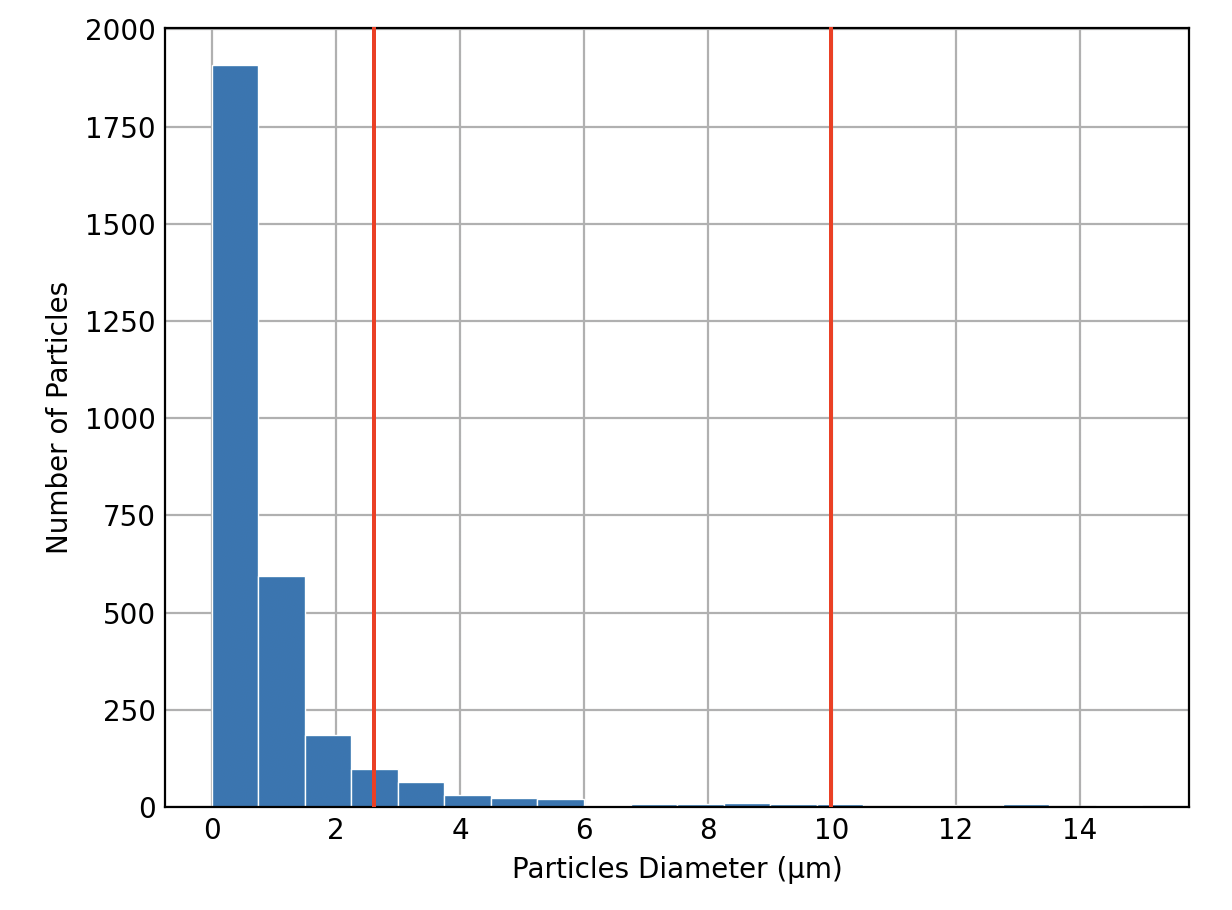
\includegraphics[width=1\linewidth]{images/Ypsilon_Ant_D.png}
  \caption{Ypsilon Ant}
  \label{fig:ypsilonant}
\end{subfigure}%
\begin{subfigure}{.5\textwidth}
  \centering
  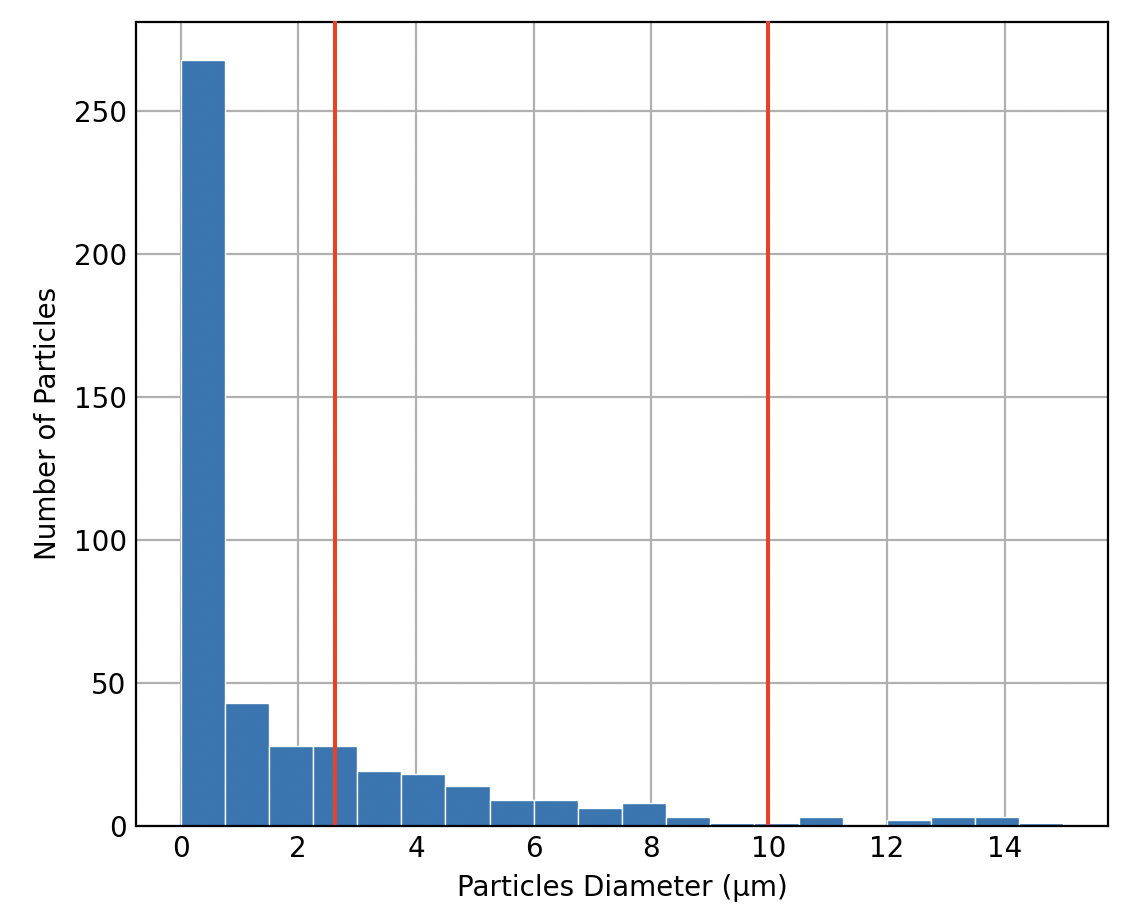
\includegraphics[width=0.9\linewidth]{images/Ypsilon_Post_D.png}
  \caption{Ypsilon Post}
  \label{fig:ypsilonpost}
\end{subfigure}
\caption{Diameter distribution histograms of Ypsilon sample}
\label{fig:4}
\end{figure}

\begin{figure}[H]
\centering
\begin{subfigure}{.5\textwidth}
  \centering
  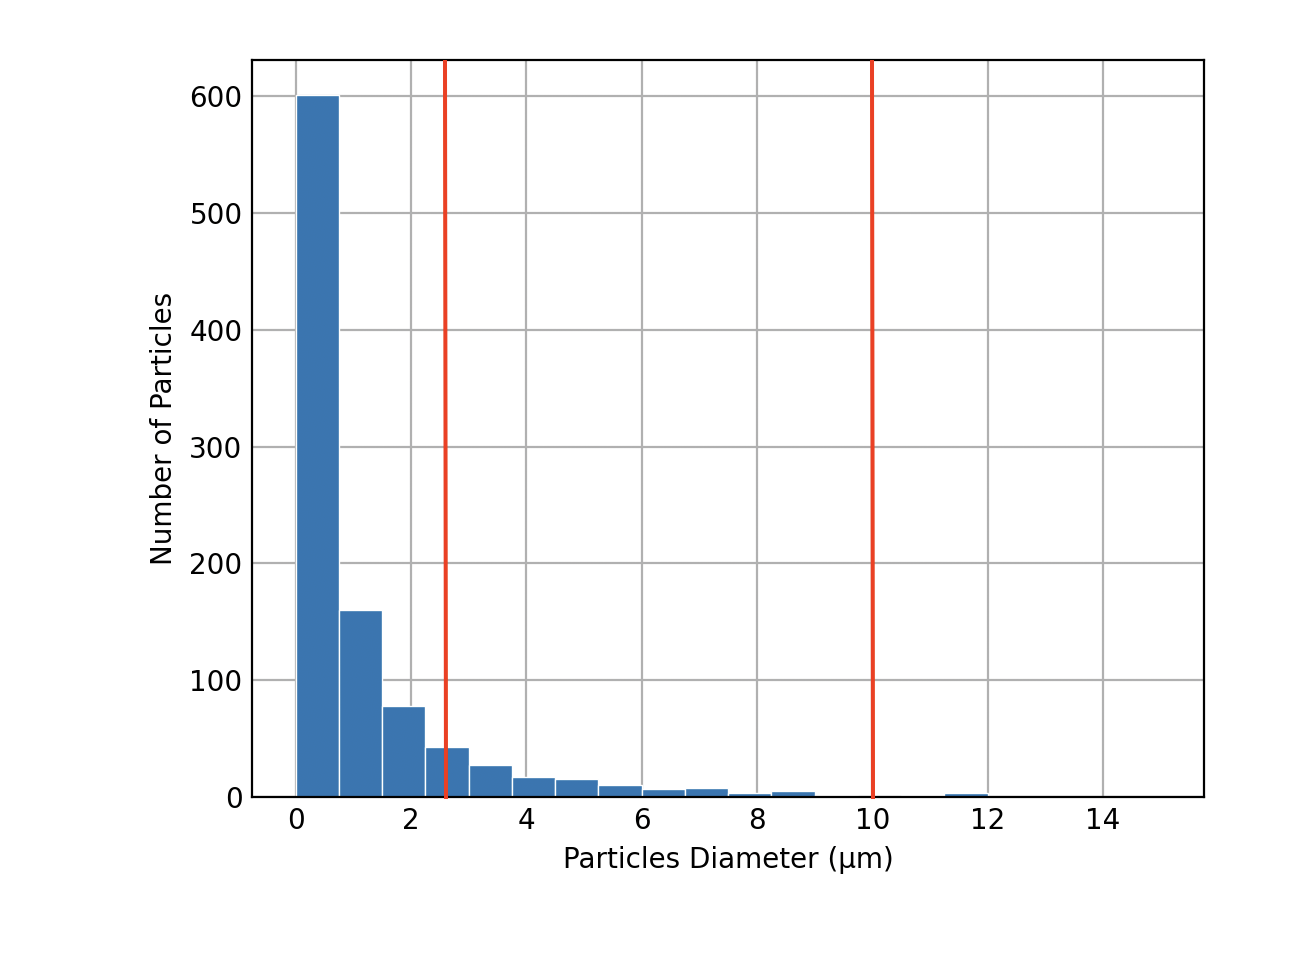
\includegraphics[width=1\linewidth]{images/corolla_ant_dis.png}
  \caption{Corolla Ant}
  \label{fig:corollaant}
\end{subfigure}%
\begin{subfigure}{.5\textwidth}
  \centering
  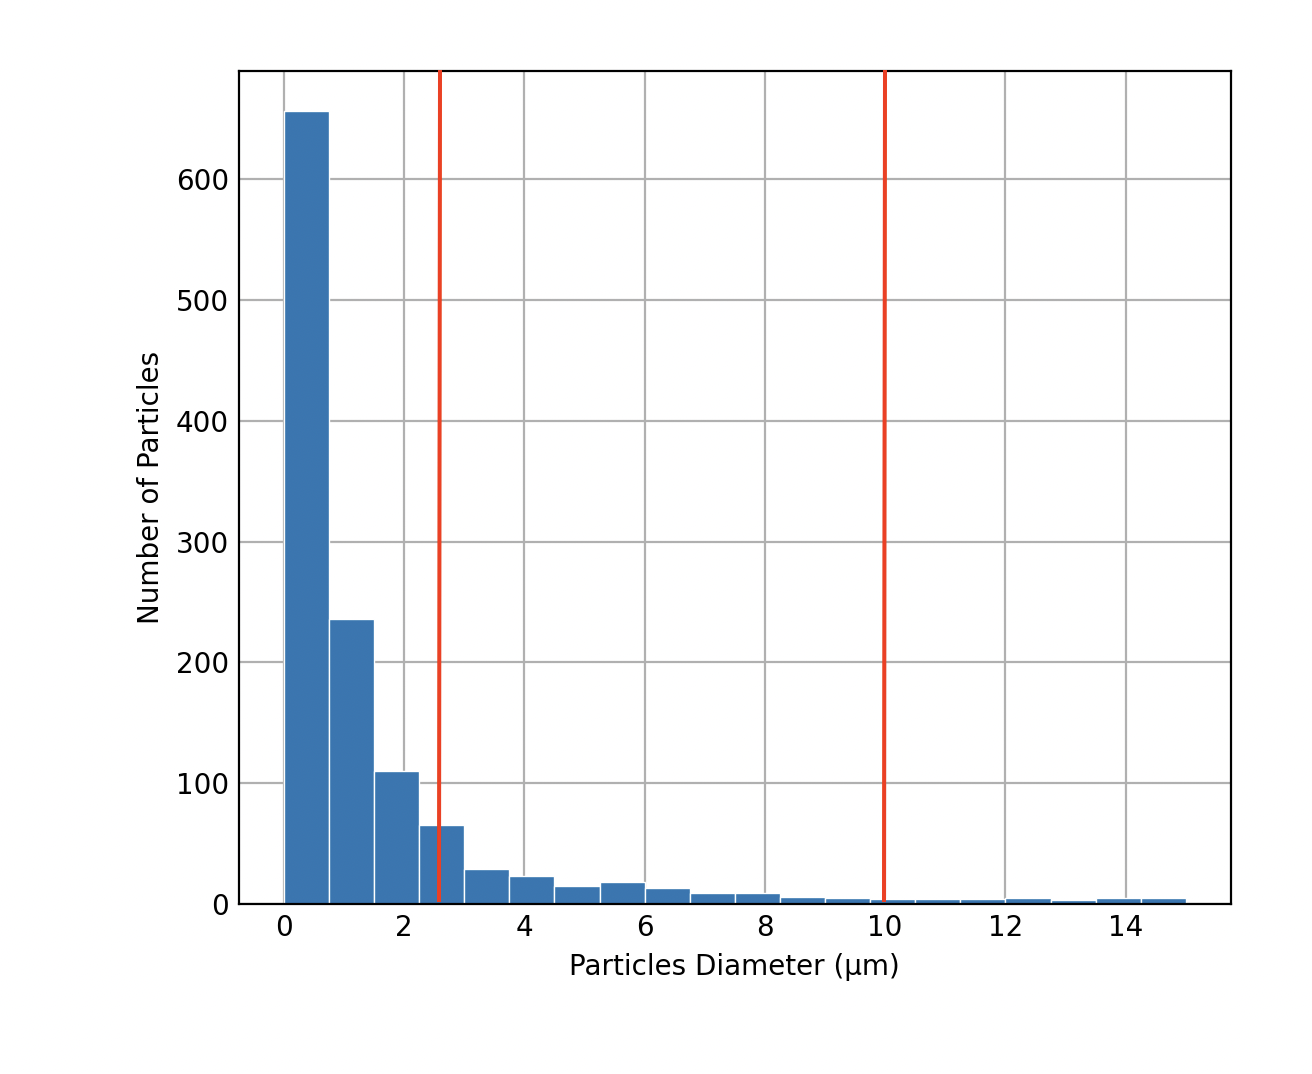
\includegraphics[width=0.9\linewidth]{images/corolla_post_dis.png}
  \caption{Corolla Post}
  \label{fig:corollapost}
\end{subfigure}
\caption{Diameter distribution histograms of Corolla sample}
\label{fig:5}
\end{figure}


The number of total particles identified in each sample was different and to ensure comparability among them, the values obtained from the measurements were transformed into percentages. This approach allowed for a uniform evaluation of the differences between the samples. \\
The percentages, shown in Table \ref{tab:percentages}, refer to the different samples and the particles (p) within the illustrated range of diameter. 

\begin{table}[h]
\centering

\begin{tabular}{l r r r r r}
\hline

Sample & $p \leq 2.5 \mu m$ & $ 2.5 \mu m < p \leq 10 \mu m$ & $p \leq 10 \mu m$ \\

\hline

Panda\_Ant & $80\%$ & $18\%$ & $2\%$ \\
Panda\_Post & $66\%$ & $13\%$ & $21\%$ \\
500X\_Ant & $90\%$ & $9\%$ & $1\%$ \\
500X\_Post & $85\%$ & $12\%$ & $3\%$ \\
500L\_Ant & $79\%$ & $20\%$ & $1\%$ \\
500L\_Post & $66\%$ & $30\%$ & $4\%$ \\
Ypsilon\_Ant & $88\%$ & $8\%$ & $4\%$ \\
Ypsilon\_Post & $72\%$ & $22\%$ & $6\%$ \\
Corolla\_Ant & $87\%$ & $12\%$ & $1\%$ \\
Corolla\_Post & $83\%$ & $12\%$ & $4\%$ \\

        \hline

    \end{tabular}
     \caption{Percentages of particles (p) found in the different samples with focus on the diameters of interest. }
     \label{tab:percentages}
\end{table}

\subsection{Heavy Metals Content}

A grouped bar chart was generated using the results obtained from EDX analysis to compare the presence of various heavy metals in each sample. \\
The x-axis denotes the sample, while the y-axis indicates the frequency, out of 100 occurrences per sample, of each specific heavy metal detected.


\begin{figure}[H]
\centering
    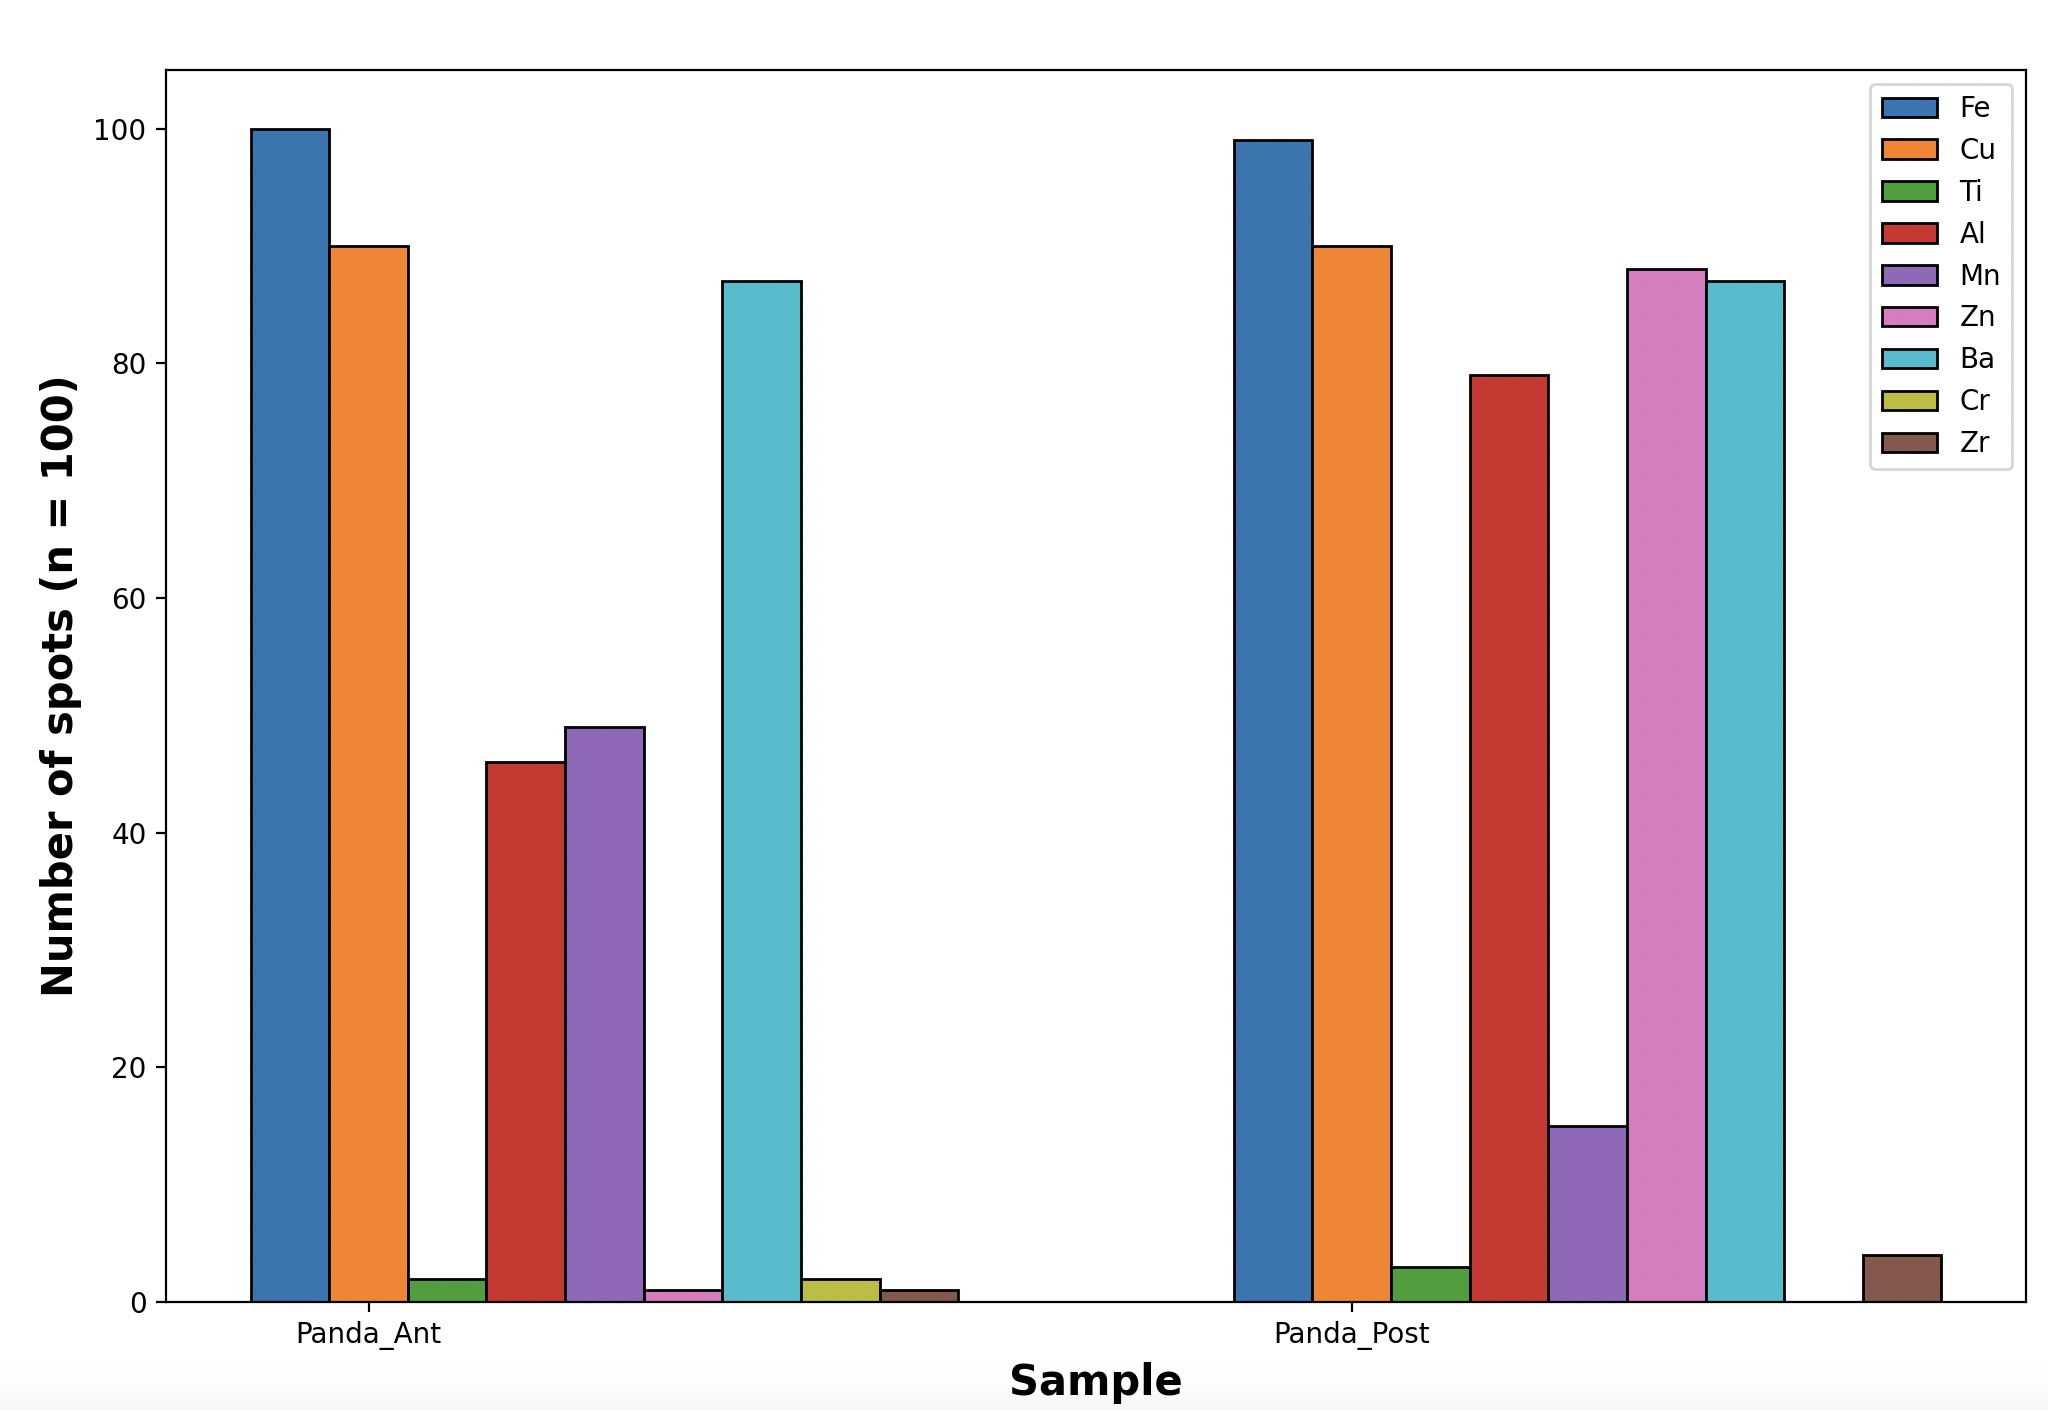
\includegraphics[scale=0.27]{images/Panda_HM.png}
    \caption{Grouped bar chart of Panda sample.}
    \label{fig:Panda_HM}
\end{figure} 

\begin{figure}[H]
\centering
    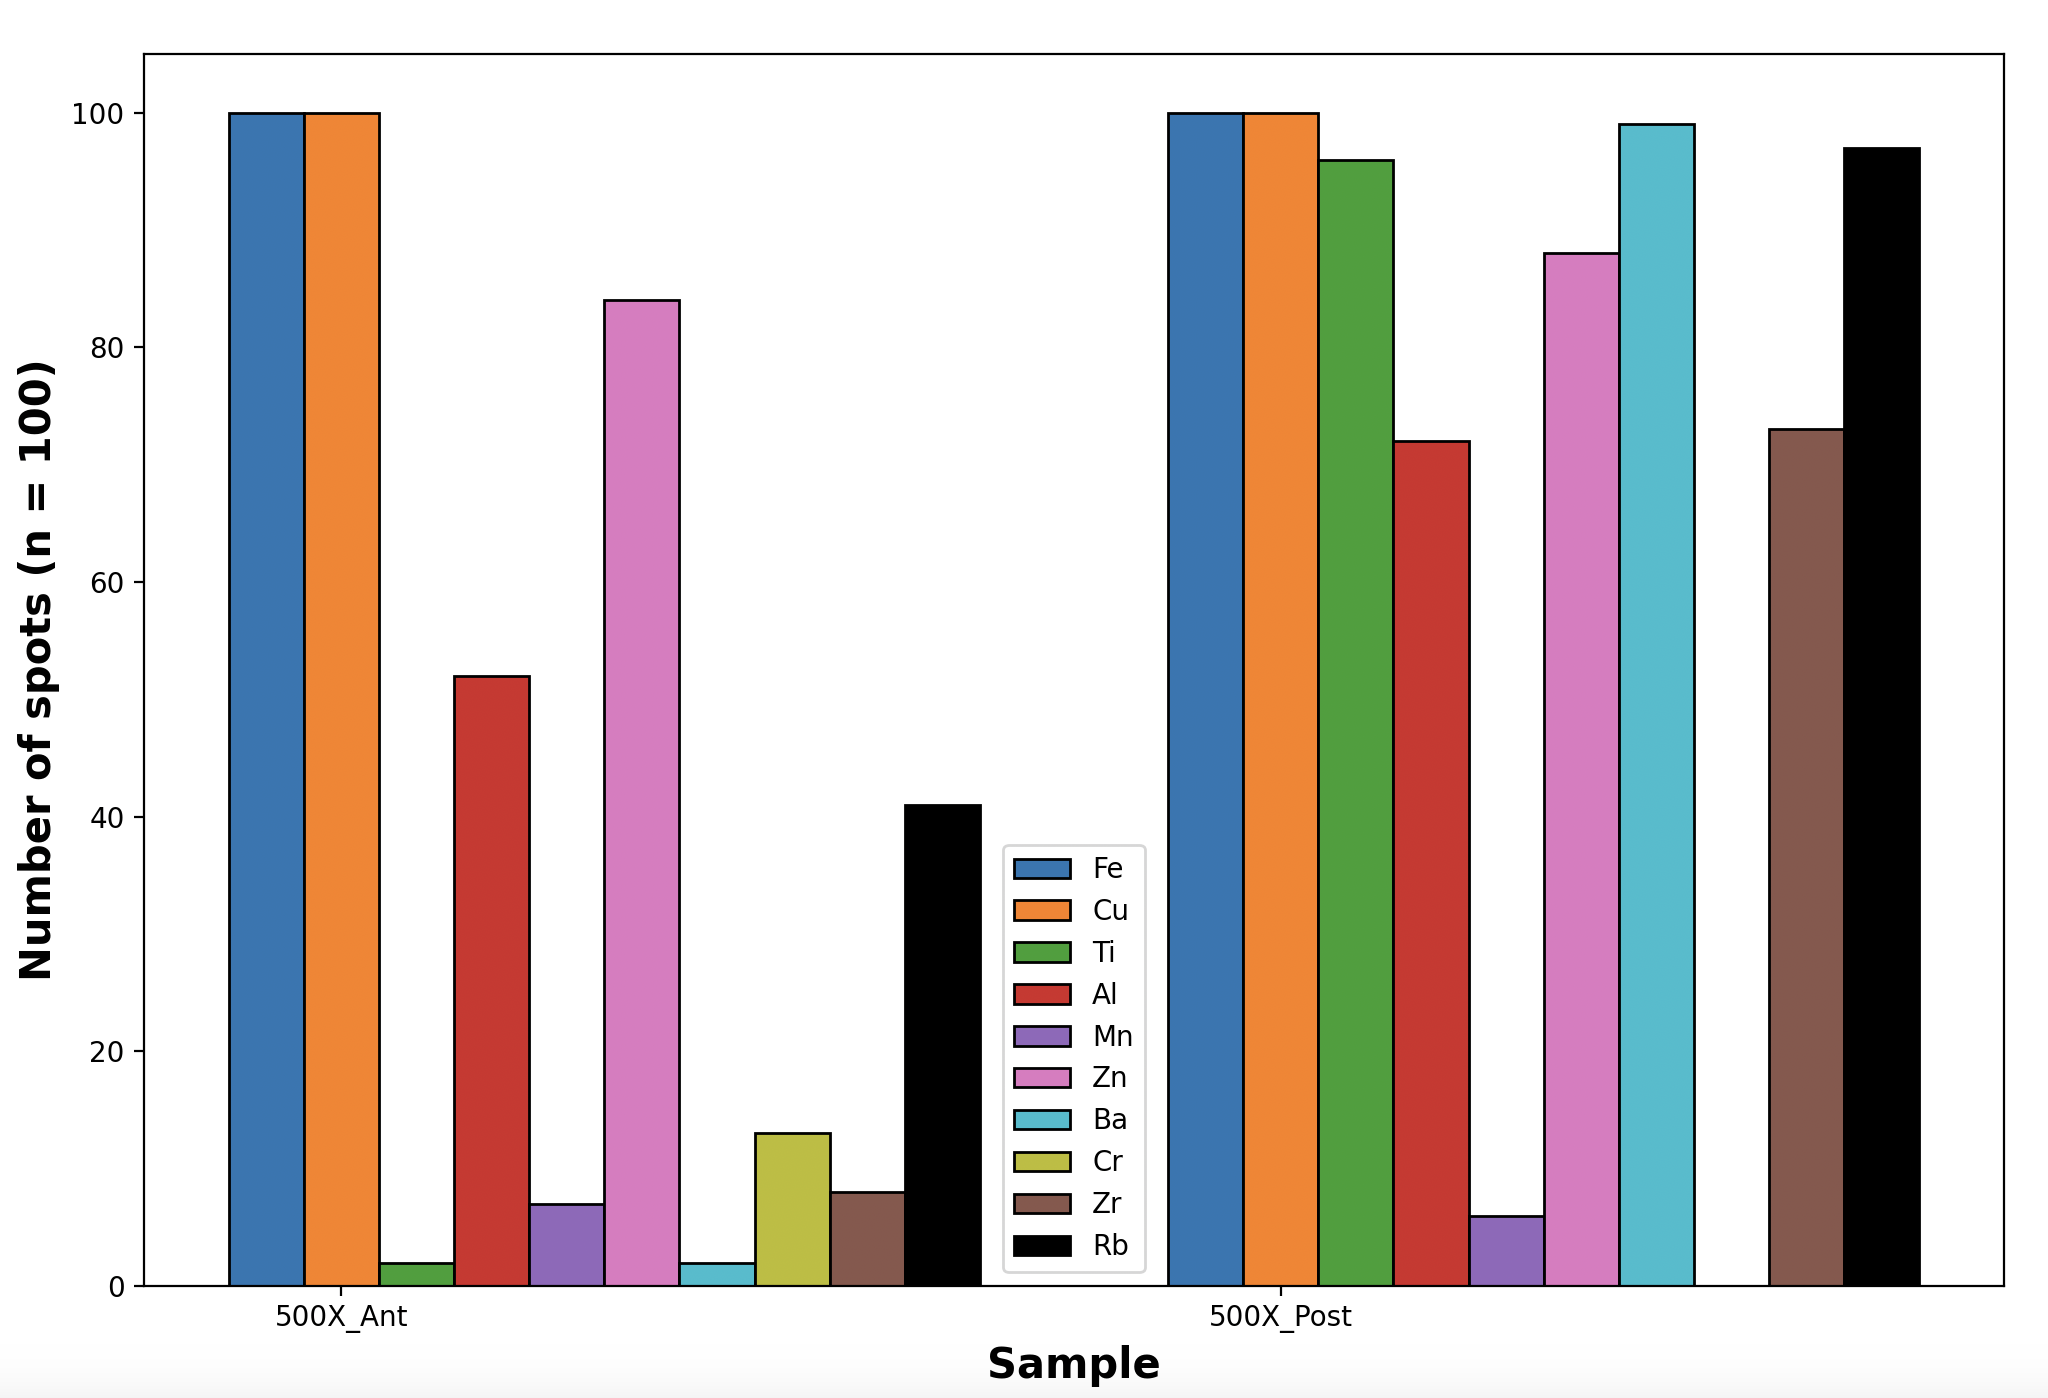
\includegraphics[scale=0.27]{images/500X_HM.png}
    \caption{Grouped bar chart of 500X sample.}
    \label{fig:500X_HM}
\end{figure} 

\begin{figure}[H]
\centering
    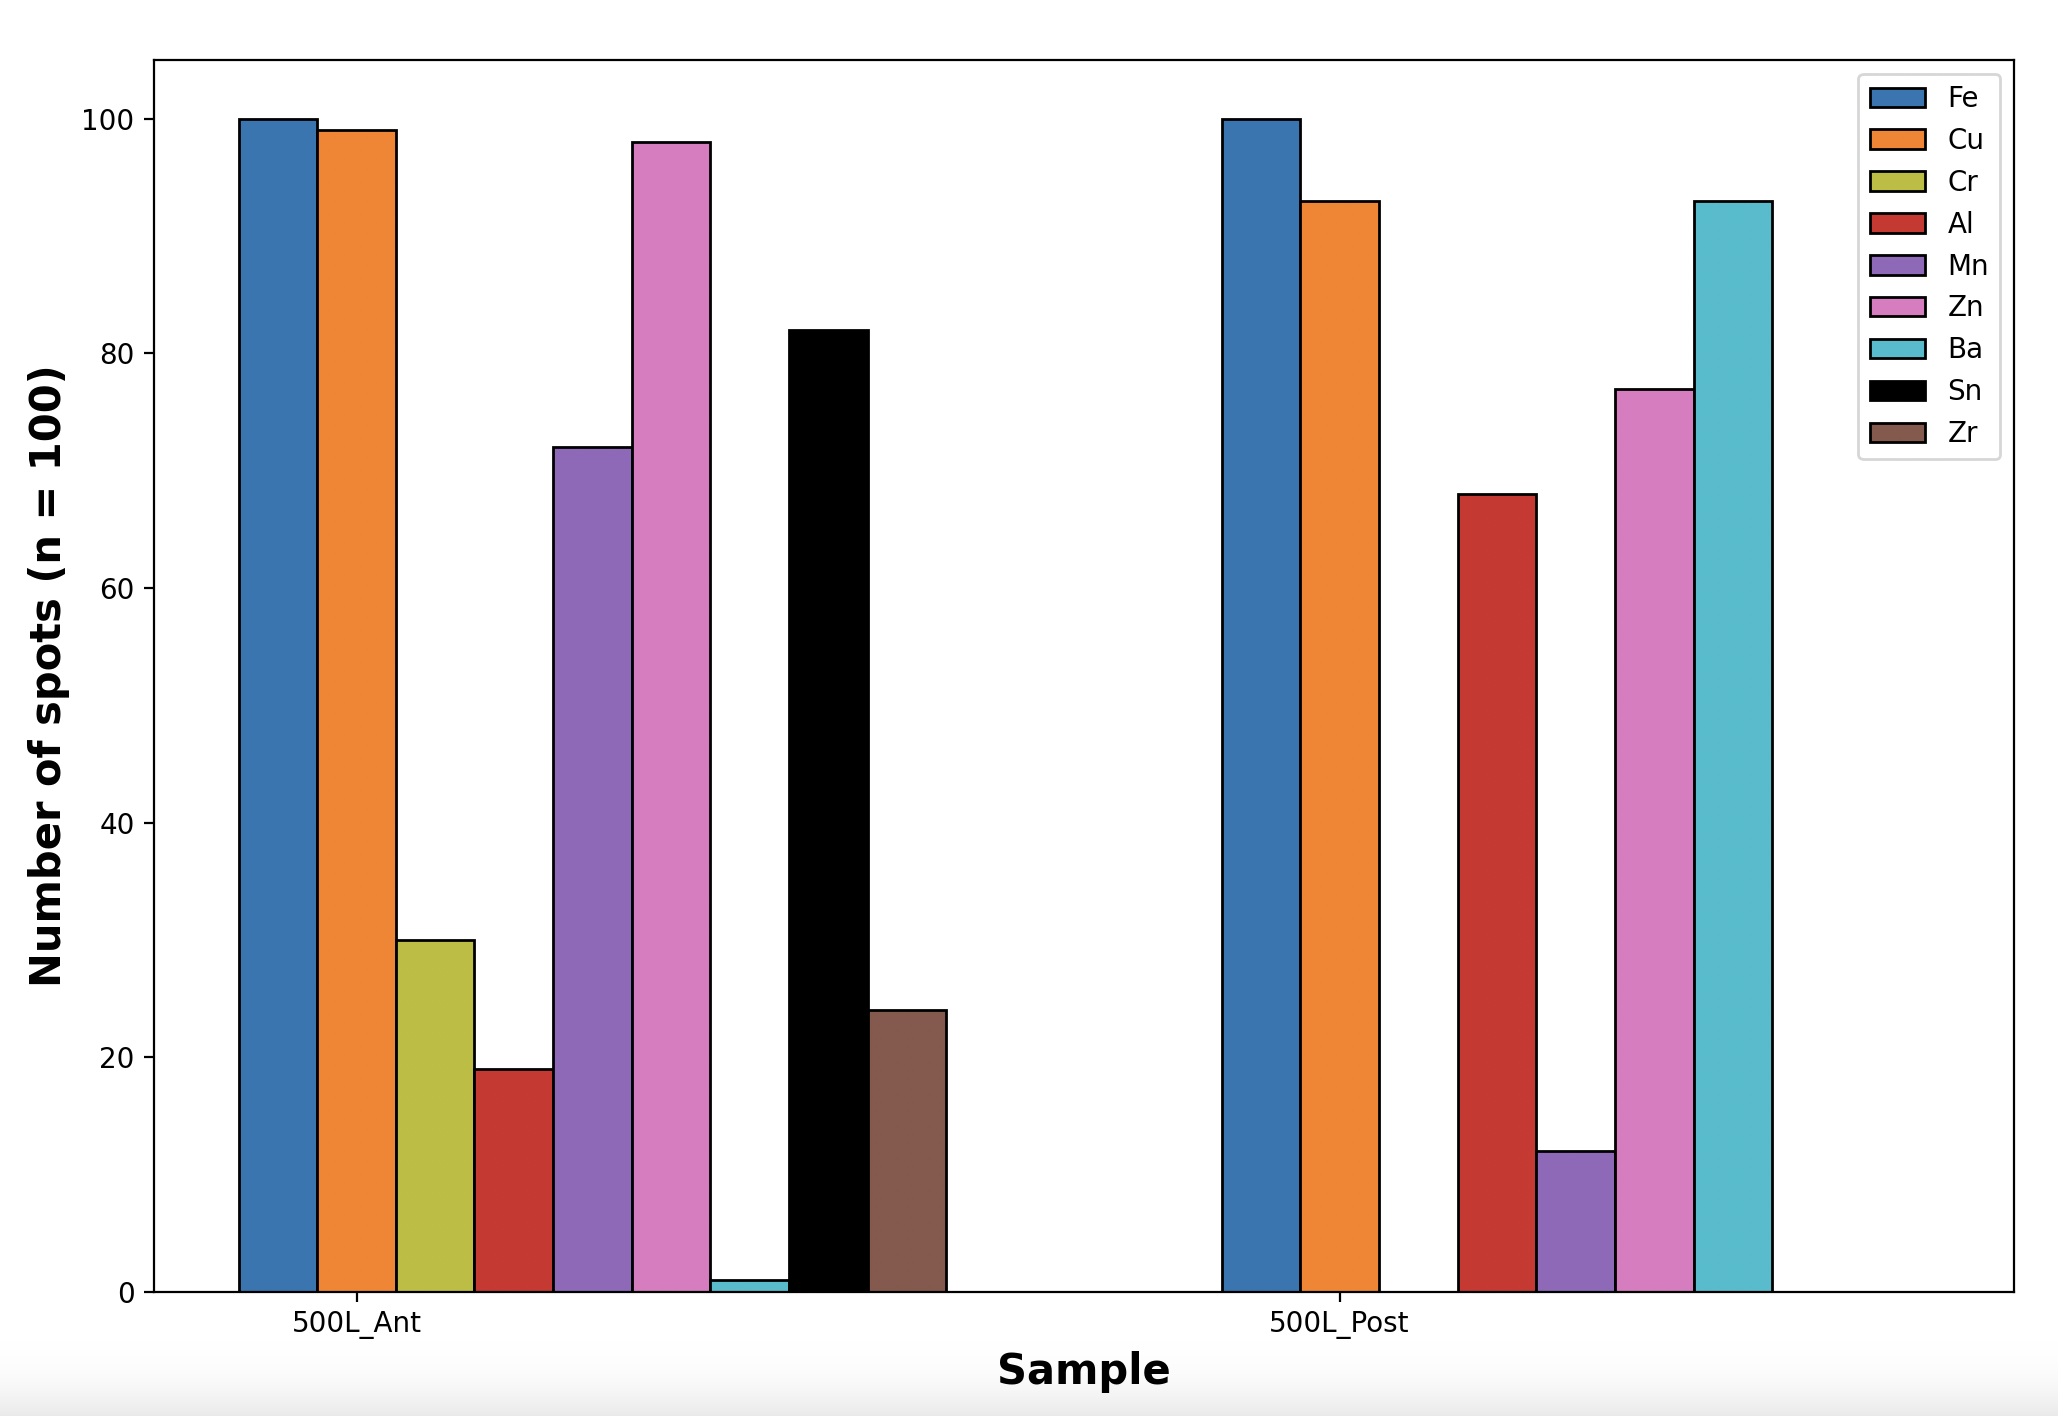
\includegraphics[scale=0.27]{images/500L_HM.png}
    \caption{Grouped bar chart of 500L sample.}
    \label{fig:500L_HM}
\end{figure} 

\begin{figure}[H]
\centering
    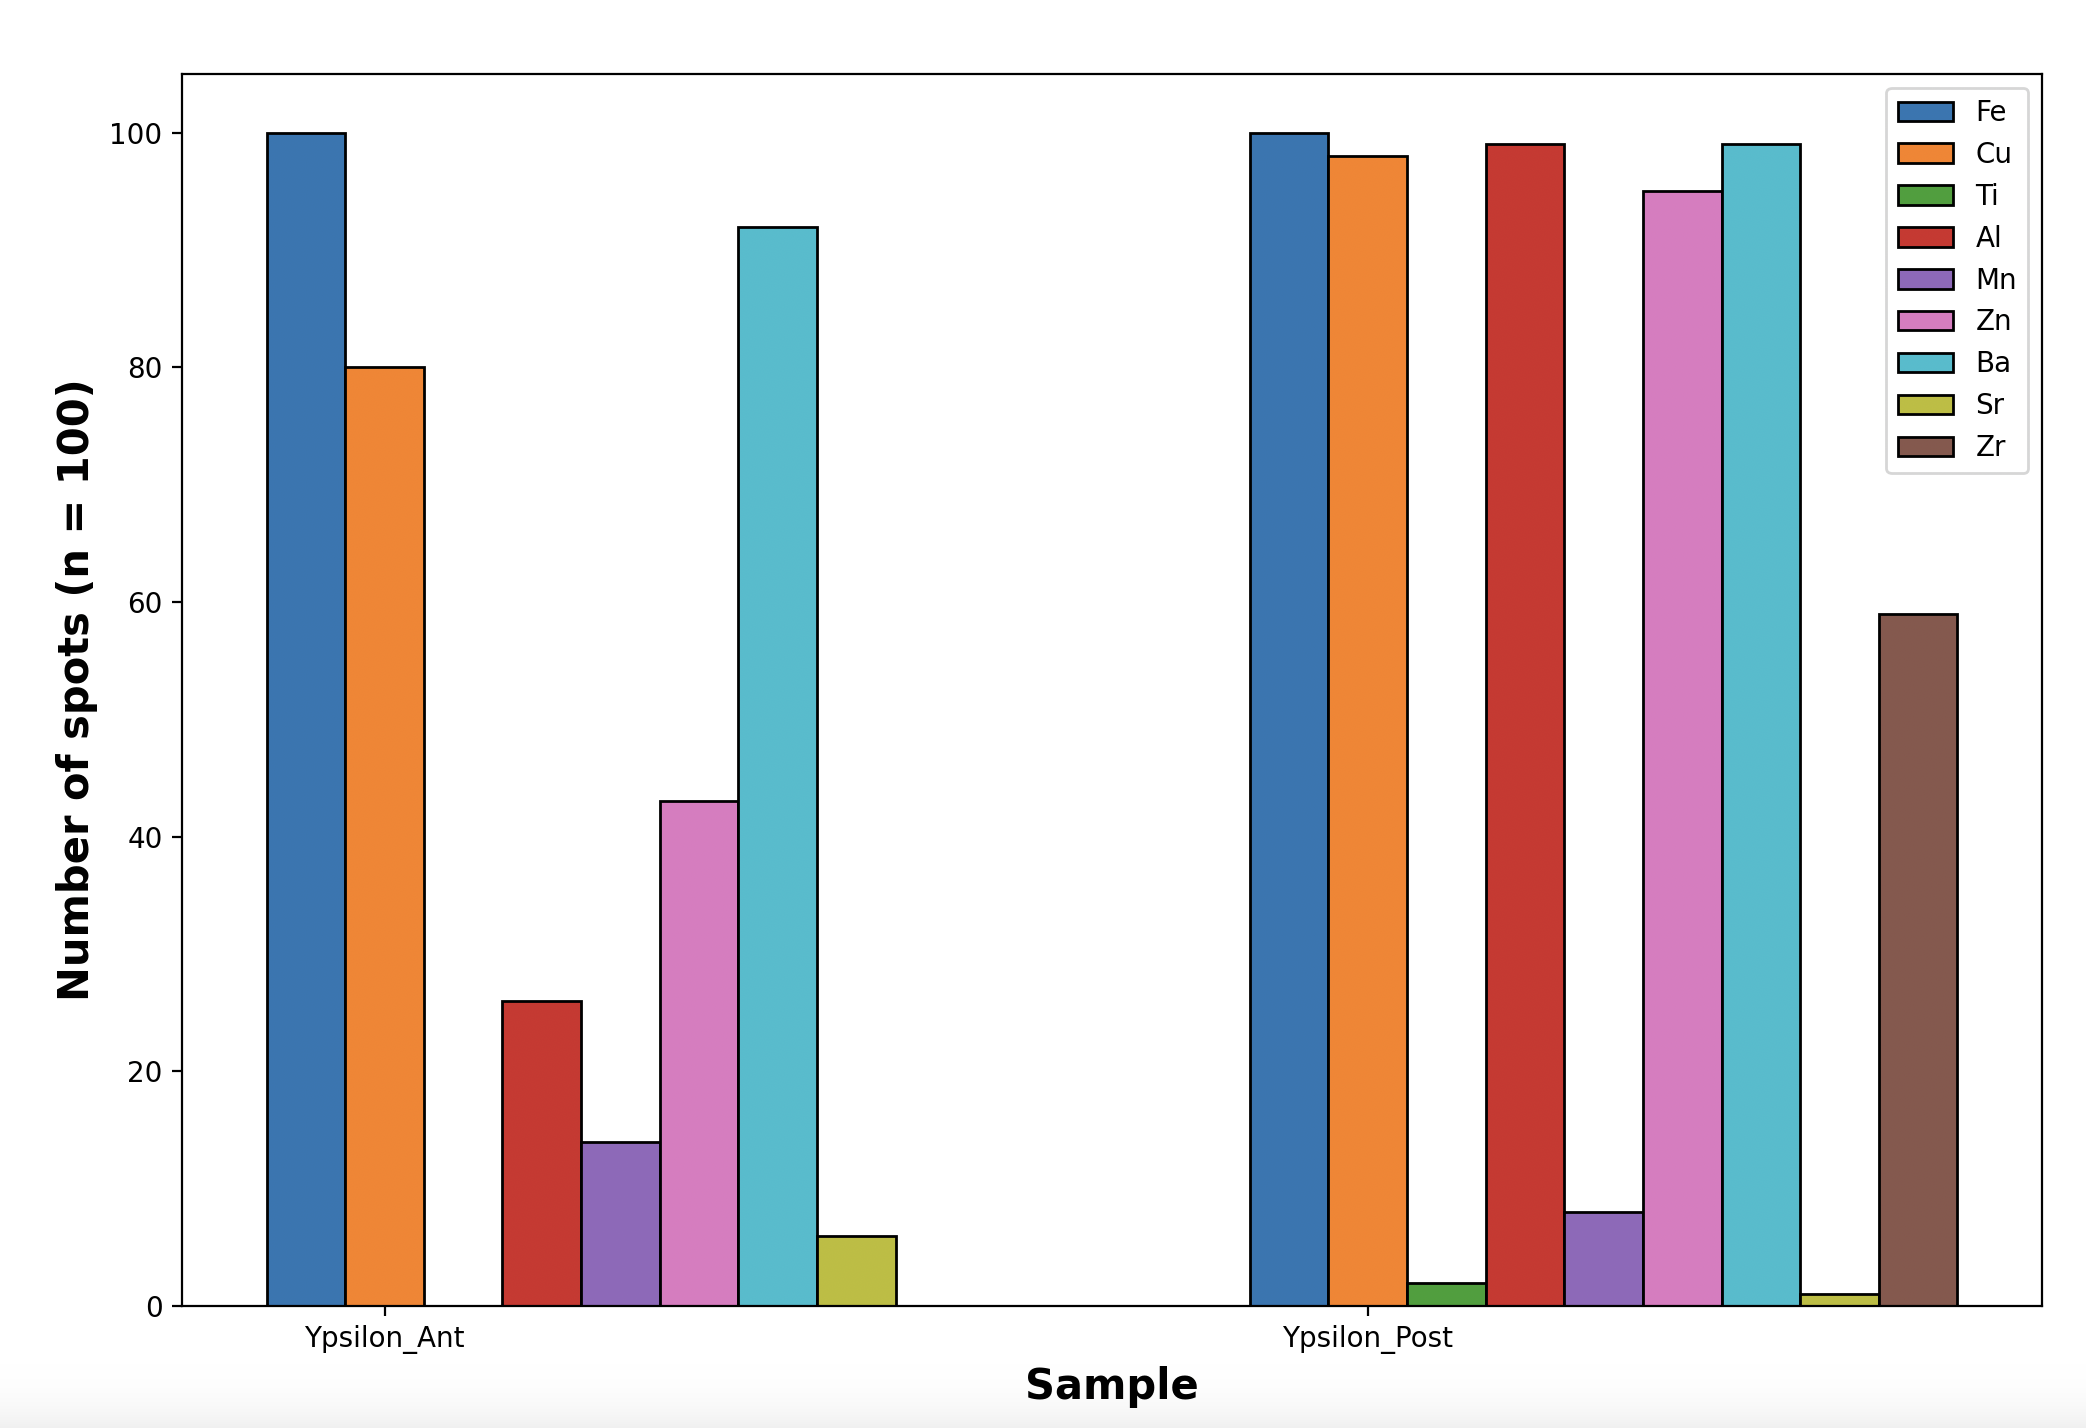
\includegraphics[scale=0.27]{images/Ypsilon_HM.png}
    \caption{Grouped bar chart of Ypsilon sample.}
    \label{fig:Ypsilon_HM}
\end{figure} 

\begin{figure}[H]
\centering
    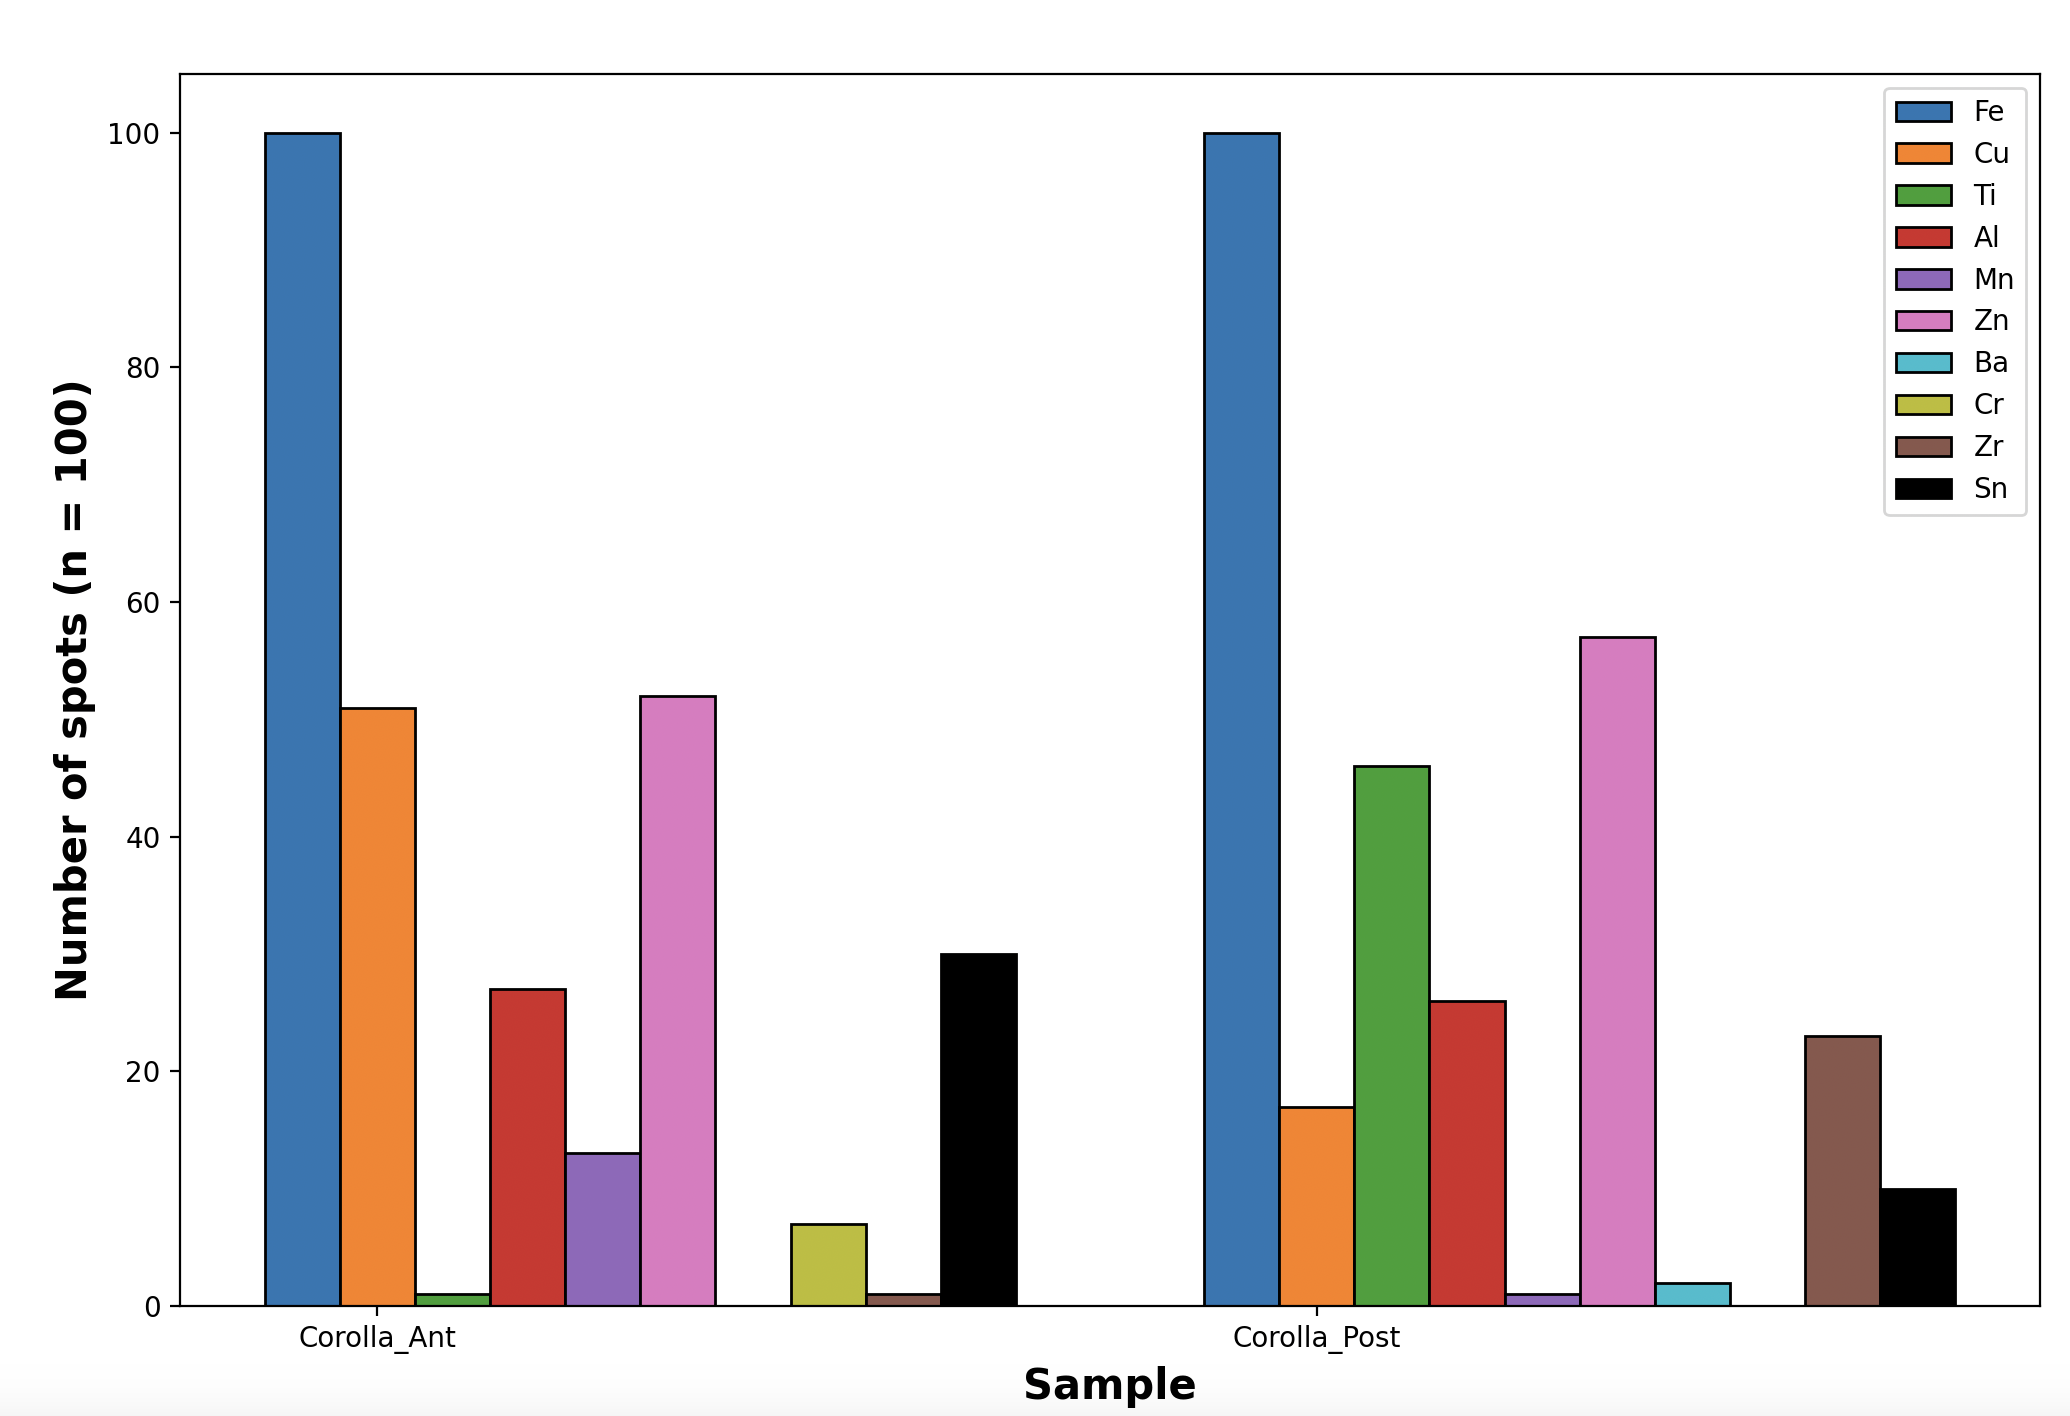
\includegraphics[scale=0.27]{images/Corolla_HM.png}
    \caption{Grouped bar chart of Corolla sample.}
    \label{fig:Corolla_HM}
\end{figure} 

\subsection{Chemical Analysis}

The chemical analysis was performed on a total of 10 sites per sample. Each site revealed a variety of elements, with some present in higher quantities than others. \\
To summarize the chemical composition of the samples, only the elements present in higher quantities and at more sites were considered. For each element, the mean of the different measurements was calculated, followed by the standard deviation ($\sigma (n-1)$) to assess the variation in the quantity of the element from the mean.\\
In each table, powders from the anterior (Ant) and posterior (Post) brakes of the same car were displayed together. If a specific element was detected in only one of the two samples, the symbol '-' was used to indicate its absence in the other one.

\begin{table}[H]\centering
  \begin{tabular}{lcccc}
    \toprule
    \multirow{2}{*}[-0.5\dimexpr \aboverulesep + \belowrulesep + \cmidrulewidth]{Panda}
    & \multicolumn{2}{c}{Ant} & \multicolumn{2}{c}{Post} \\
    \cmidrule(l){2-3} \cmidrule(l){4-5}
    & Mean (wt\%) & $\sigma (n-1)$ & Mean (wt\%) & $\sigma (n-1)$ \\
    \midrule
    O & 30.64 & 3.81 & 41.67 & 13.07 \\
    Na & 3.77 & 4.22 & 1.76 & 3.50 \\
    Mg & 0.43 & 0.75 & - & - \\
    Al & 1.32 & 4.06 & 1.81 & 1.40 \\
    Si & 4.34 & 1.34 & 3.66 & 1.60 \\
    P & 0.90 & 0.28 & 0.38 & 0.42 \\
    S & 5.01 & 3.78 & 3.74 & 4.60 \\
    Ca & 0.83 & 0.65 & 2.94 & 1.66 \\
    Mn & 0.30 & 0.32 & 0.06 & 0.16 \\
    Fe & 49.15 & 12.09 & 38.90 & 14.02 \\
    Cu & 0.91 & 0.44 & 1.25 & 2.21 \\
    Zn & - & - & 1.02 & 0.49 \\
    Ba & 2.84 & 4.87 & 2.13 & 1.16 \\
    \bottomrule
  \end{tabular}
    \caption{Main elements detected into the samples Panda Ant and Post, with mean and $\sigma (n-1)$.}
    \label{fig:Elements_Panda}
\end{table}

\begin{table}[H]\centering
  \begin{tabular}{lcccc}
    \toprule
    \multirow{2}{*}[-0.5\dimexpr \aboverulesep + \belowrulesep + \cmidrulewidth]{500X}
    & \multicolumn{2}{c}{Ant} & \multicolumn{2}{c}{Post} \\
    \cmidrule(l){2-3} \cmidrule(l){4-5}
    & Mean (wt\%) & $\sigma (n-1)$ & Mean (wt\%) & $\sigma (n-1)$ \\
    \midrule
    O & 45.17 & 11.66 & 48.88 & 9.15 \\
    Na & 0.76 & 2.07 & 0.67 & 1.41 \\
    Mg & 0.47 & 0.84 & - & - \\
    Al & 0.73 & 1.00 & 0.87 & 0.62 \\
    Si & 3.44 & 5.85 & 3.52 & 1.57 \\
    P & 0.22 & 0.37 & - & - \\
    S & 3.30 & 4.78 & 3.97 & 1.43 \\
    Cl & - & - & 0.42 & 0.35 \\
    Ca & 0.37 & 0.21 & 1.10 & 1.71 \\
    Fe & 41.07 & 13.04 & 19.45 & 12.00 \\
    Cu & 2.48 & 0.99 & 6.86 & 7.46 \\
    Zn & 0.90 & 0.55 & 2.19 & 0.77 \\
    Zr & 0.20 & 1.11 & 1.62 & 2.64 \\
    Sn & 0.29 & 0.37 & 2.42 & 1.82 \\
    Ba & - & - & 6.50 & 2.98 \\
    \bottomrule
  \end{tabular}
    \caption{Main elements detected into the samples 500X Ant and Post, with mean and $\sigma (n-1)$.}
    \label{fig:Elements_500X}
\end{table}

\begin{table}[H]\centering
  \begin{tabular}{lcccc}
    \toprule
    \multirow{2}{*}[-0.5\dimexpr \aboverulesep + \belowrulesep + \cmidrulewidth]{500L}
    & \multicolumn{2}{c}{Ant} & \multicolumn{2}{c}{Post} \\
    \cmidrule(l){2-3} \cmidrule(l){4-5}
    & Mean (wt\%) & $\sigma (n-1)$ & Mean (wt\%) & $\sigma (n-1)$ \\
    \midrule
    O & 41.90 & 11.19 & 30.82 & 3.31 \\
    Na & 1.12 & 3.65 & 2.34 & 4.03 \\
    Al & 0.38 & 2.00 & 1.75 & 1.32 \\
    Si & 3.02 & 3.88 & 4.10 & 2.54 \\
    P & 0.32 & 0.35 & - & - \\
    S & 2.75 & 2.86 & 5.40 & 2.81 \\
    Cl & 0.29 & 0.35 & - & - \\
    Cr & 0.05 & 0.09 & - & - \\
    Ca & - & - & 2.53 & 0.70 \\
    Mn & 0.30 & 0.20 & - & - \\
    Fe & 42.25 & 13.85 & 47.56 & 8.14 \\
    Cu & 3.33 & 1.20 & 1.17 & 0.40 \\
    Zn & 2.43 & 3.93 & 0.82 & 0.52 \\
    Zr & 0.76 & 3.81 & - & - \\
    Sn & 0.88 & 1.21 & - & - \\
    Ba & - & - & 3.13 & 1.42 \\
    \bottomrule
  \end{tabular}
    \caption{Main elements detected into the samples 500L Ant and Post, with mean and $\sigma (n-1)$.}
    \label{fig:Elements_500L}
\end{table}

\begin{table}[H]\centering
  \begin{tabular}{lcccc}
    \toprule
    \multirow{2}{*}[-0.5\dimexpr \aboverulesep + \belowrulesep + \cmidrulewidth]{Ypsilon}
    & \multicolumn{2}{c}{Ant} & \multicolumn{2}{c}{Post} \\
    \cmidrule(l){2-3} \cmidrule(l){4-5}
    & Mean (wt\%) & $\sigma (n-1)$ & Mean (wt\%) & $\sigma (n-1)$ \\
    \midrule
    O & 29.29 & 2.30 & 33.47 & 4.08 \\
    Na & 1.73 & 2.92 & 1.21 & 2.39 \\
    Mg & 1.56 & 1.63 & 1.09 & 2.28 \\
    Al & 0.31 & 0.76 & 4.50 & 3.32 \\
    Si & 3.82 & 0.95 & 7.59 & 6.22 \\
    P & 0.14 & 0.28 & 0.98 & 1.85 \\
    S & 4.27 & 2.34 & 3.31 & 2.08 \\
    Cl & 0.08 & 0.23 & 0.77 & 0.60 \\
    K & - & - & 1.39 & 2.80 \\
    Ca & 0.80 & 3.31 & 5.40 & 5.08 \\
    Mn & 0.07 & 0.17 & 0.04 & 0.23 \\
    Fe & 54.31 & 9.84 & 28.80 & 10.37 \\
    Cu & 0.56 & 0.52 & 1.45 & 0.50 \\
    Zn & 0.35 & 0.55 & 2.12 & 1.07 \\
    Zr & - & - & 0.94 & 0.98 \\
    Ba & 2.25 & 3.93 & 5.86 & 2.33 \\
    \bottomrule
  \end{tabular}
    \caption{Main elements detected into the samples Ypsilon Ant and Post, with mean and $\sigma (n-1)$.}
    \label{fig:Elements_Ypsilon}
\end{table}

\begin{table}[H]\centering
  \begin{tabular}{lcccc}
    \toprule
    \multirow{2}{*}[-0.5\dimexpr \aboverulesep + \belowrulesep + \cmidrulewidth]{Corolla}
    & \multicolumn{2}{c}{Ant} & \multicolumn{2}{c}{Post} \\
    \cmidrule(l){2-3} \cmidrule(l){4-5}
    & Mean (wt\%) & $\sigma (n-1)$ & Mean (wt\%) & $\sigma (n-1)$ \\
    \midrule
    O & 29.72 & 3.60 & 34.69 & 6.13 \\
    Na & 1.82 & 3.58 & 0.80 & 2.32 \\
    Mg & 0.26 & 1.25 & 3.53 & 6.96 \\
    Al & 1.05 & 4.42 & 1.15 & 2.83 \\
    Si & 3.81 & 2.49 & 9.55 & 6.73 \\
    P & 0.52 & 0.72 & 0.48 & 2.01 \\
    S & 4.03 & 3.10 & 3.43 & 2.95 \\
    Cl & - & - & 0.67 & 3.09 \\
    K & - & - & 1.12 & 4.25 \\
    Ca & 0.24 & 0.34 & 4.09 & 10.18 \\
    Cr & 0.39 & 17.98 & - & - \\
    Ti & - & - & 2.82 & 4.15 \\
    Fe & 55.90 & 11.74 & 34.03 & 21.15 \\
    Cu & 1.19 & 1.96 & 0.25 & 0.64 \\
    Zn & 0.62 & 0.77 & 1.33 & 2.77 \\
    Zr & - & - & 1.44 & 4.95 \\
    Sn & 0.32 & 0.54 & 0.42 & 3.30 \\
    \bottomrule
  \end{tabular}
    \caption{Main elements detected into the samples Corolla Ant and Post, with mean and $\sigma (n-1)$.}
    \label{fig:Elements_Corolla}
\end{table}
\pagebreak

\subsection{Morphology}

All the samples exhibited a wide array of morphologies. Generally, the presence of agglomerates of particles of different sizes is very common. Given the diverse materials used in brake production, it is not surprising to find such a variety of morphologies. As previously mentioned, every component of brake pads plays a specific role in the braking system. \\
Figure \ref{fig:Layers} shows the typical composition of brake pads, highlighting that larger particles act as abrasives while smaller particles function as fillers. Elongated morphology is also common due to the presence of reinforcement fibers.

\begin{figure}[H]
\centering
    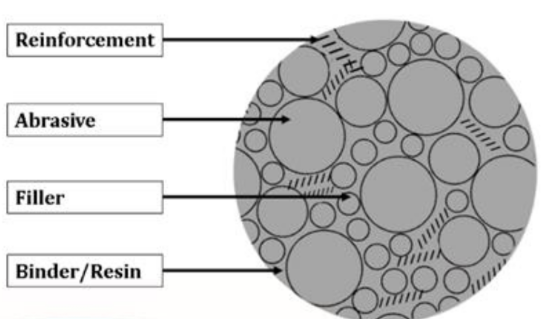
\includegraphics[scale=0.85]{images/layers.png}
    \caption{Different components present in brakes \cite{irawan2022overview}.}
    \label{fig:Layers}
\end{figure}

In general, it was observed that the concentration of nanoparticles smaller than 100 nm in brake powders increases with the temperature of the cast iron disc. Submicron particles are formed by evaporation or condensation processes, followed by the subsequent aggregation of primary nanoparticles \cite{grigoratos2015brake}.\\
During SEM observations, most of the brake components were identified in all samples and classified according to their main morphology.\\

As evidenced by recent research on the characterization of vehicle brake emissions \cite{liati2019airborne}, coarse PM ranging from 10 µm to 2.5 µm predominantly appears as aggregates composed of particles of varying sizes and irregular shapes. \\
Single coarse particles were observed less frequently than fine particles, which range between 2.5 µm and 0.1 µm and sometimes occur separated from the aggregates.
In this study, aggregates were observed in both anterior and posterior brakes and in all of the sample regardless the type of car analyzed.

\begin{figure}[H]
\centering
\begin{subfigure}{.5\textwidth}
  \centering
  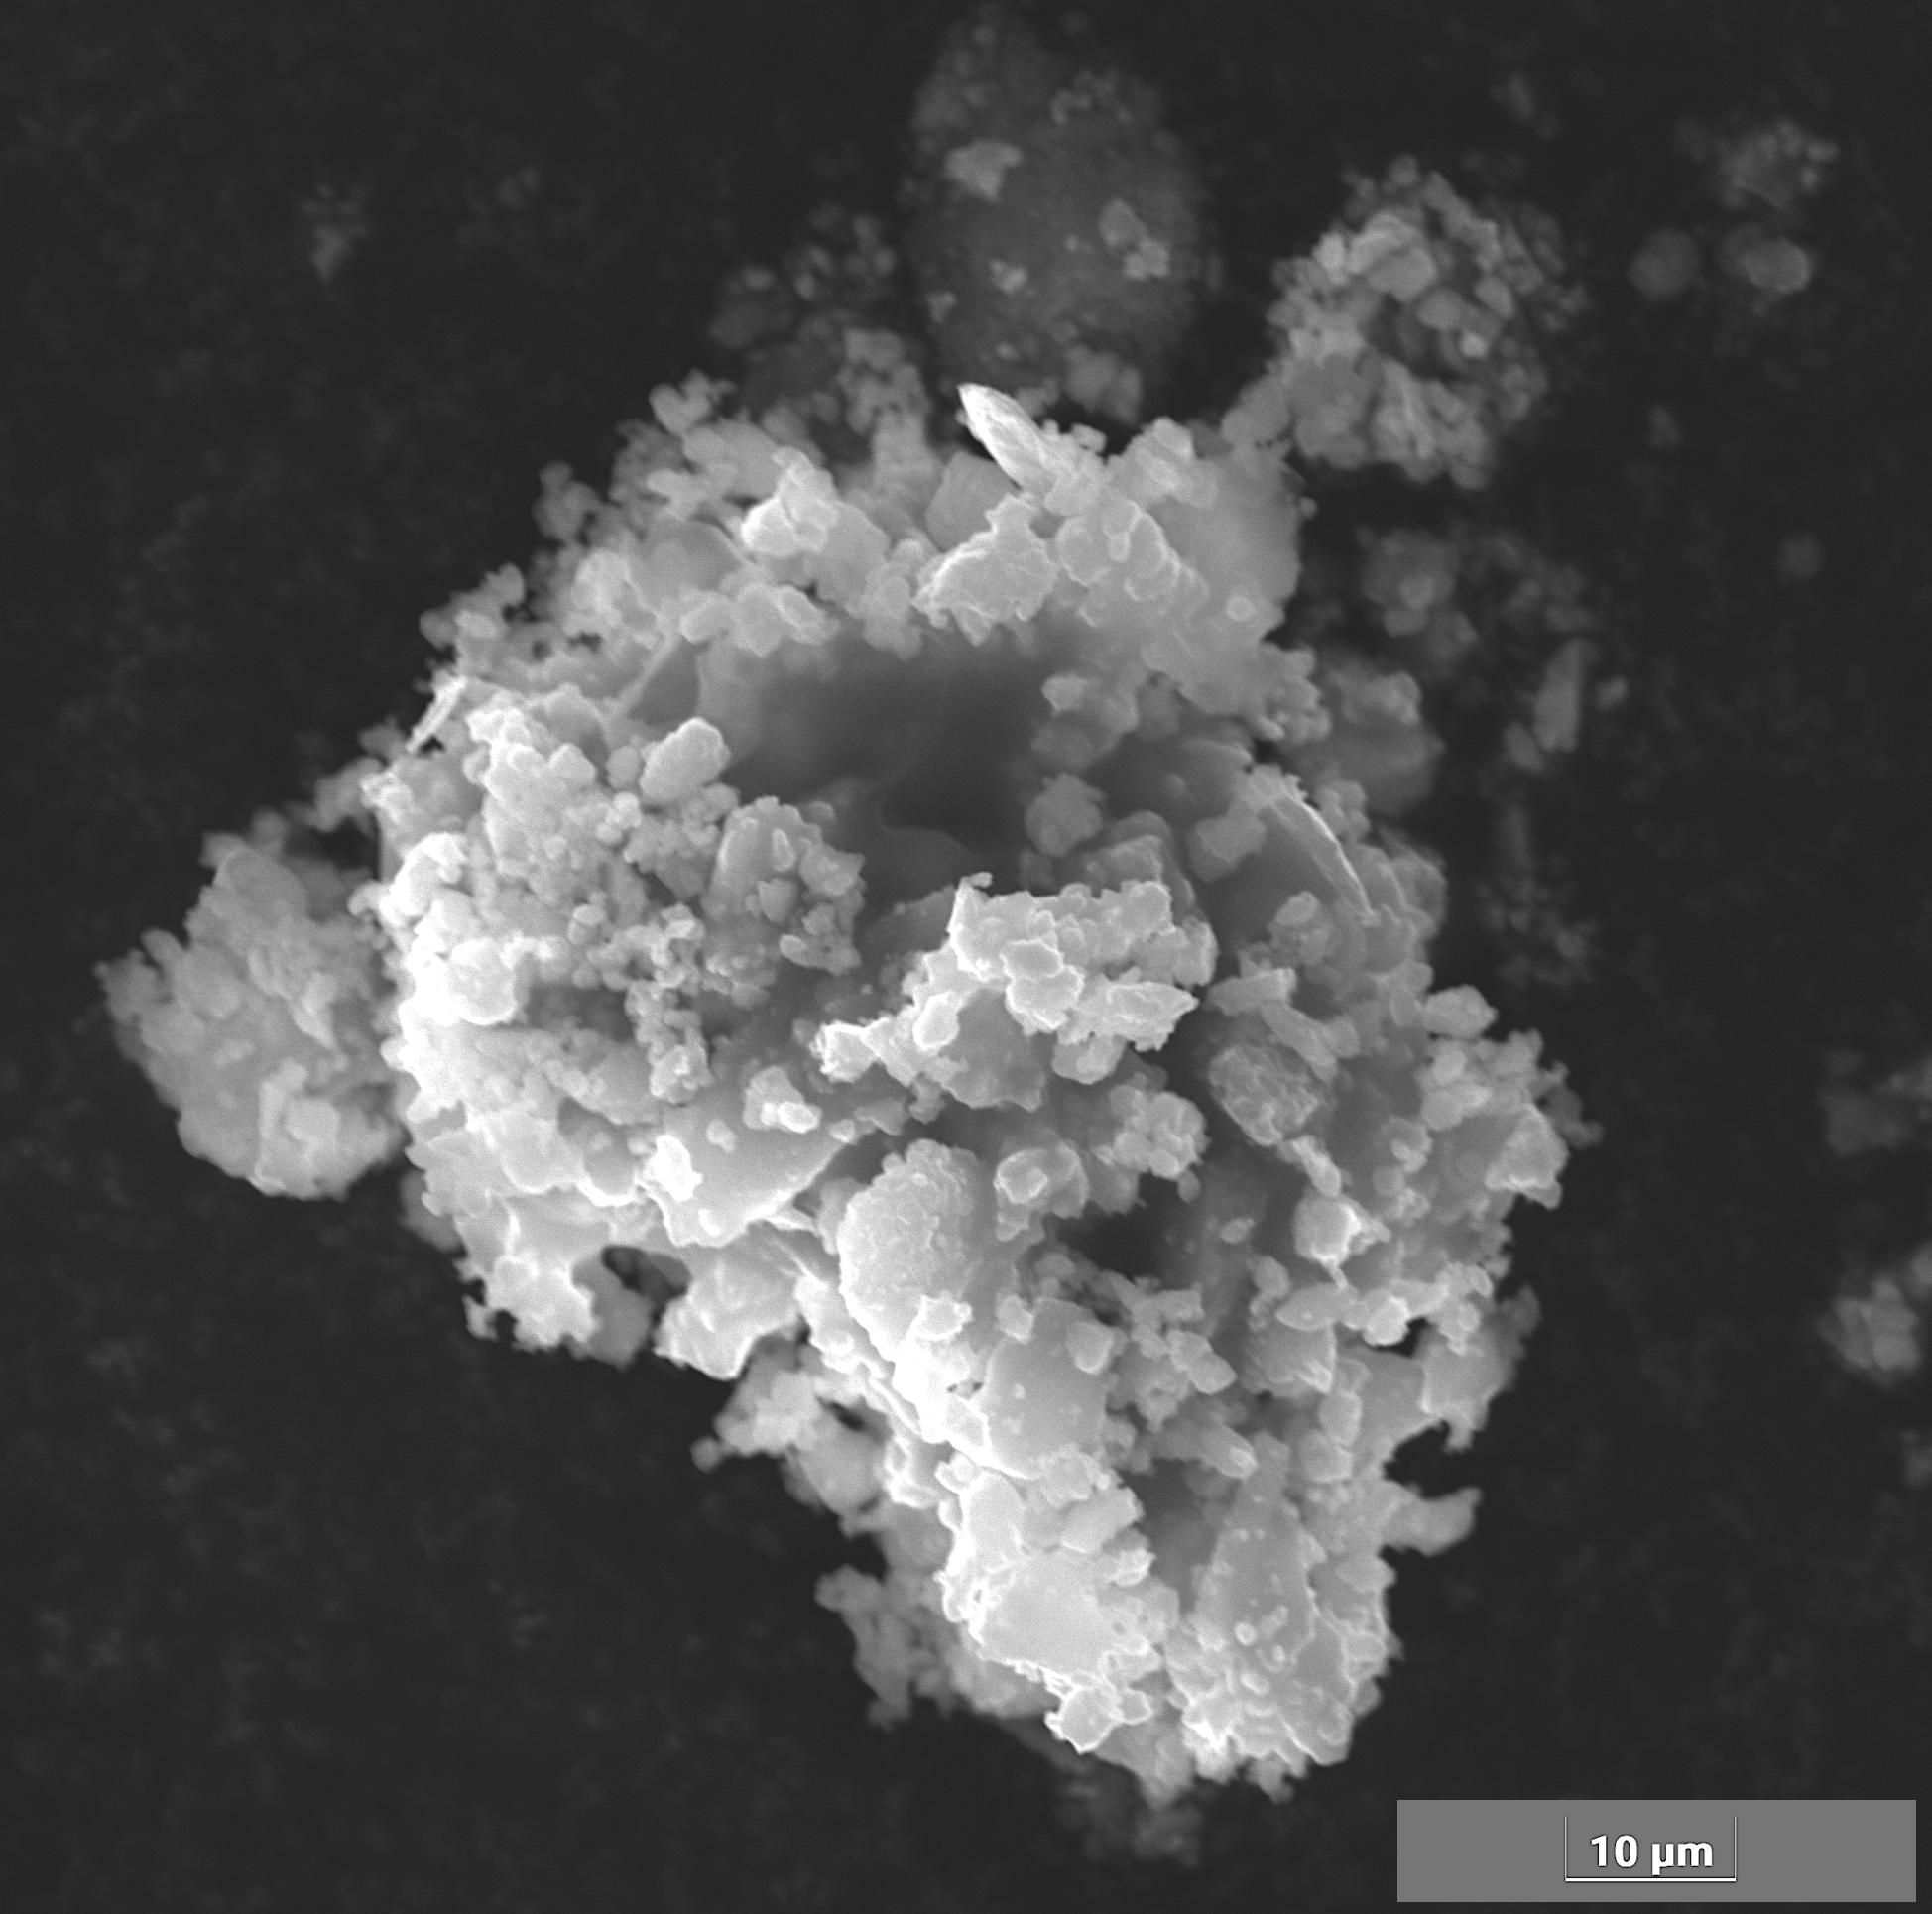
\includegraphics[width=1\linewidth]{images/500L-ANT05-copia.png}
  \caption{500L Ant}
  \label{fig:Aggregates_500L_Ant}
\end{subfigure}%
\begin{subfigure}{.5\textwidth}
  \centering
  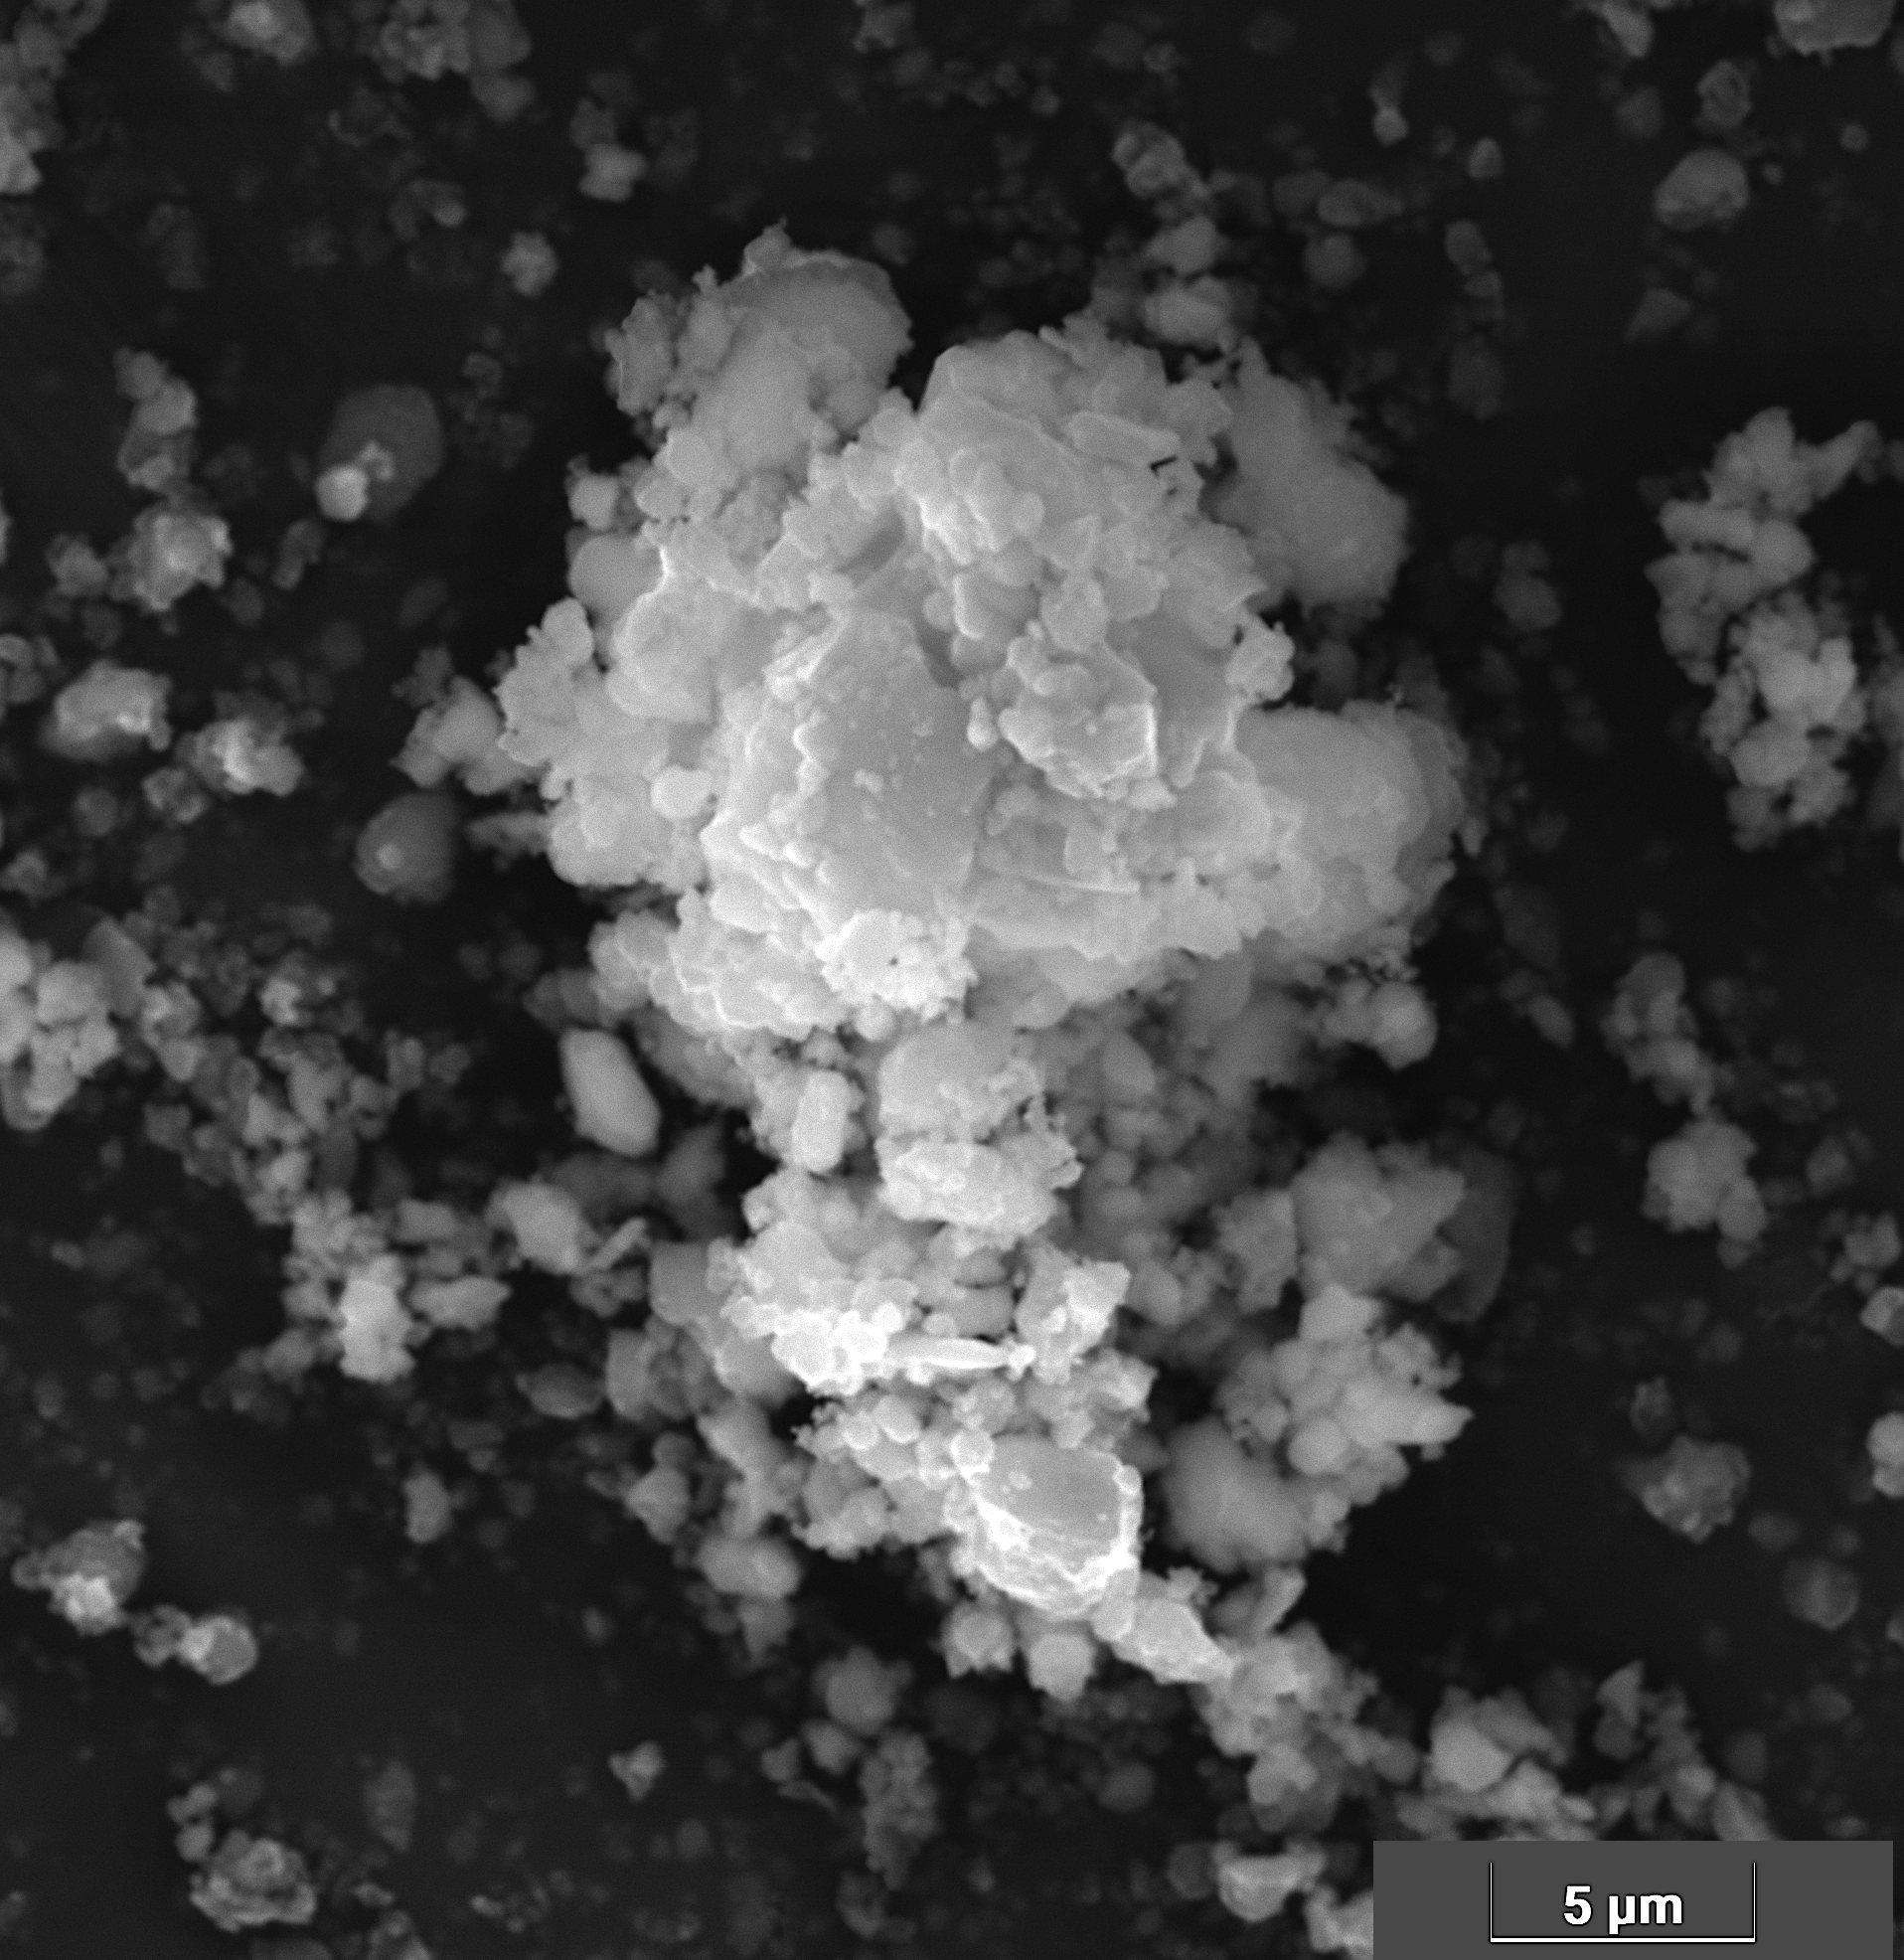
\includegraphics[width=0.97\linewidth]{images/YPSILON-ANT04.png}
  \caption{Ypsilon Ant}
  \label{fig:Aggregates_Y_Ant}
\end{subfigure}
\caption{Examples of aggregates found in the powders from anterior brakes of two different sample.}
\label{fig:Aggregates_Ant}
\end{figure}

\begin{figure}[H]
\centering
\begin{subfigure}{.5\textwidth}
  \centering
  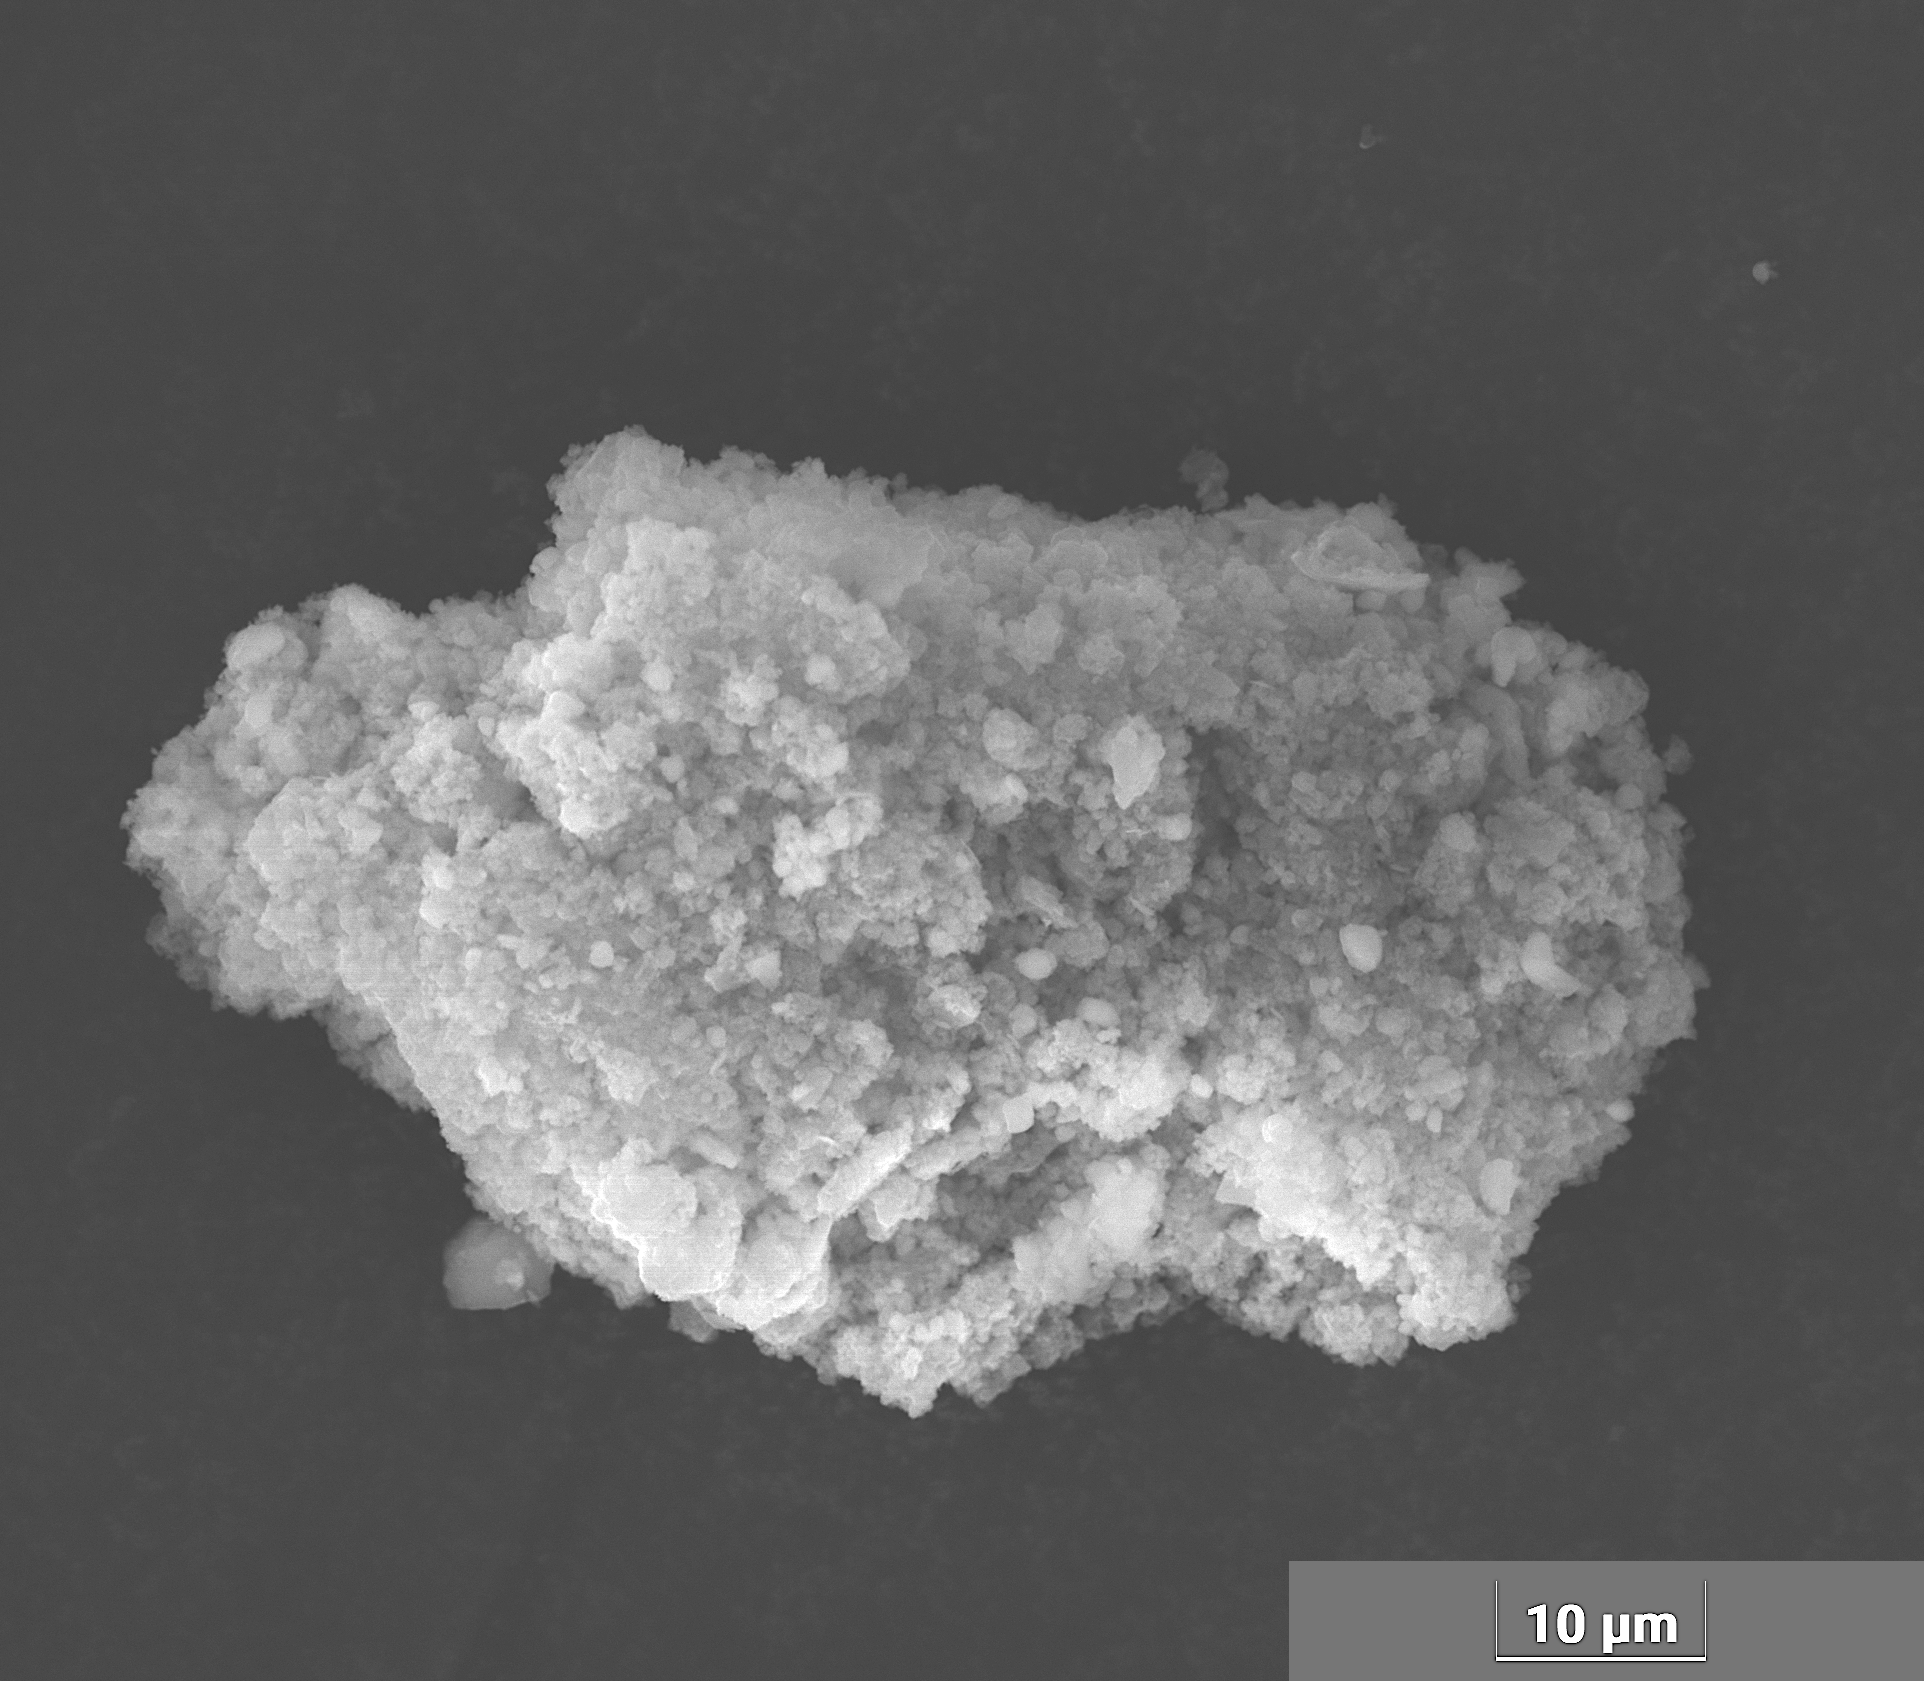
\includegraphics[width=1\linewidth]{images/COROLLA-POST01.png}
  \caption{Corolla Post}
  \label{fig:Aggregates_Corolla_Post}
\end{subfigure}%
\begin{subfigure}{.5\textwidth}
  \centering
  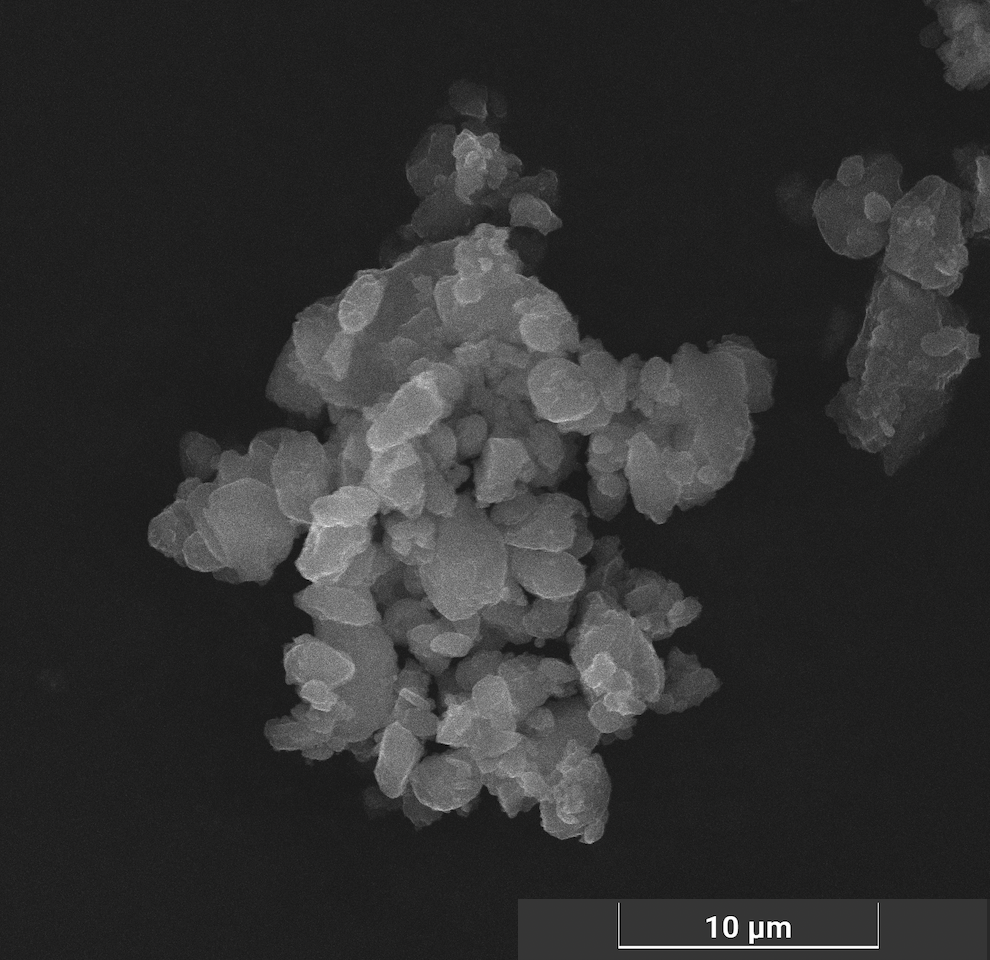
\includegraphics[width=0.9\linewidth]{images/PANDA-POST02.png}
  \caption{Panda Post}
  \label{fig:Aggregates_Panda_Post}
\end{subfigure}
\caption{Examples of aggregates found in the powders from posterior brakes of two different sample.}
\label{fig:Aggregates_Post}
\end{figure}

It is important to note that, the powders found on the surface of brakes, are synthetic material, as they are produced during braking rather than originating from natural sources. Therefore, to describe the various morphologies observed, the mechanisms by which wear debris is generated were used as a reference for this characterization .\\
In a related article such mechanisms are explained thoroughly, here an extract is reported as a reference:
\pagebreak
\blockquote[\cite{machinerylubricationAnatomyWear}]{
One of the most common ways platelet-shaped particles can occur is by normal and tangential forces through contacting asperities. \\

Wire or curl-shaped particles have been linked to cutting wear where one of the contacting surfaces possesses an asperity or lodged particle that is plastically rigid compared to the other surface from which the ribbon-shaped particle is gouged out.}

Based on this statement and another reference describing the shapes of various industrial particles \cite{ulusoy2023review}, the presence of different shapes among the samples, as shown below in Figures \ref{fig:Lamellar}, was identified.

\begin{figure}[H]
 \centering
    \begin{subfigure}{0.45\linewidth}
        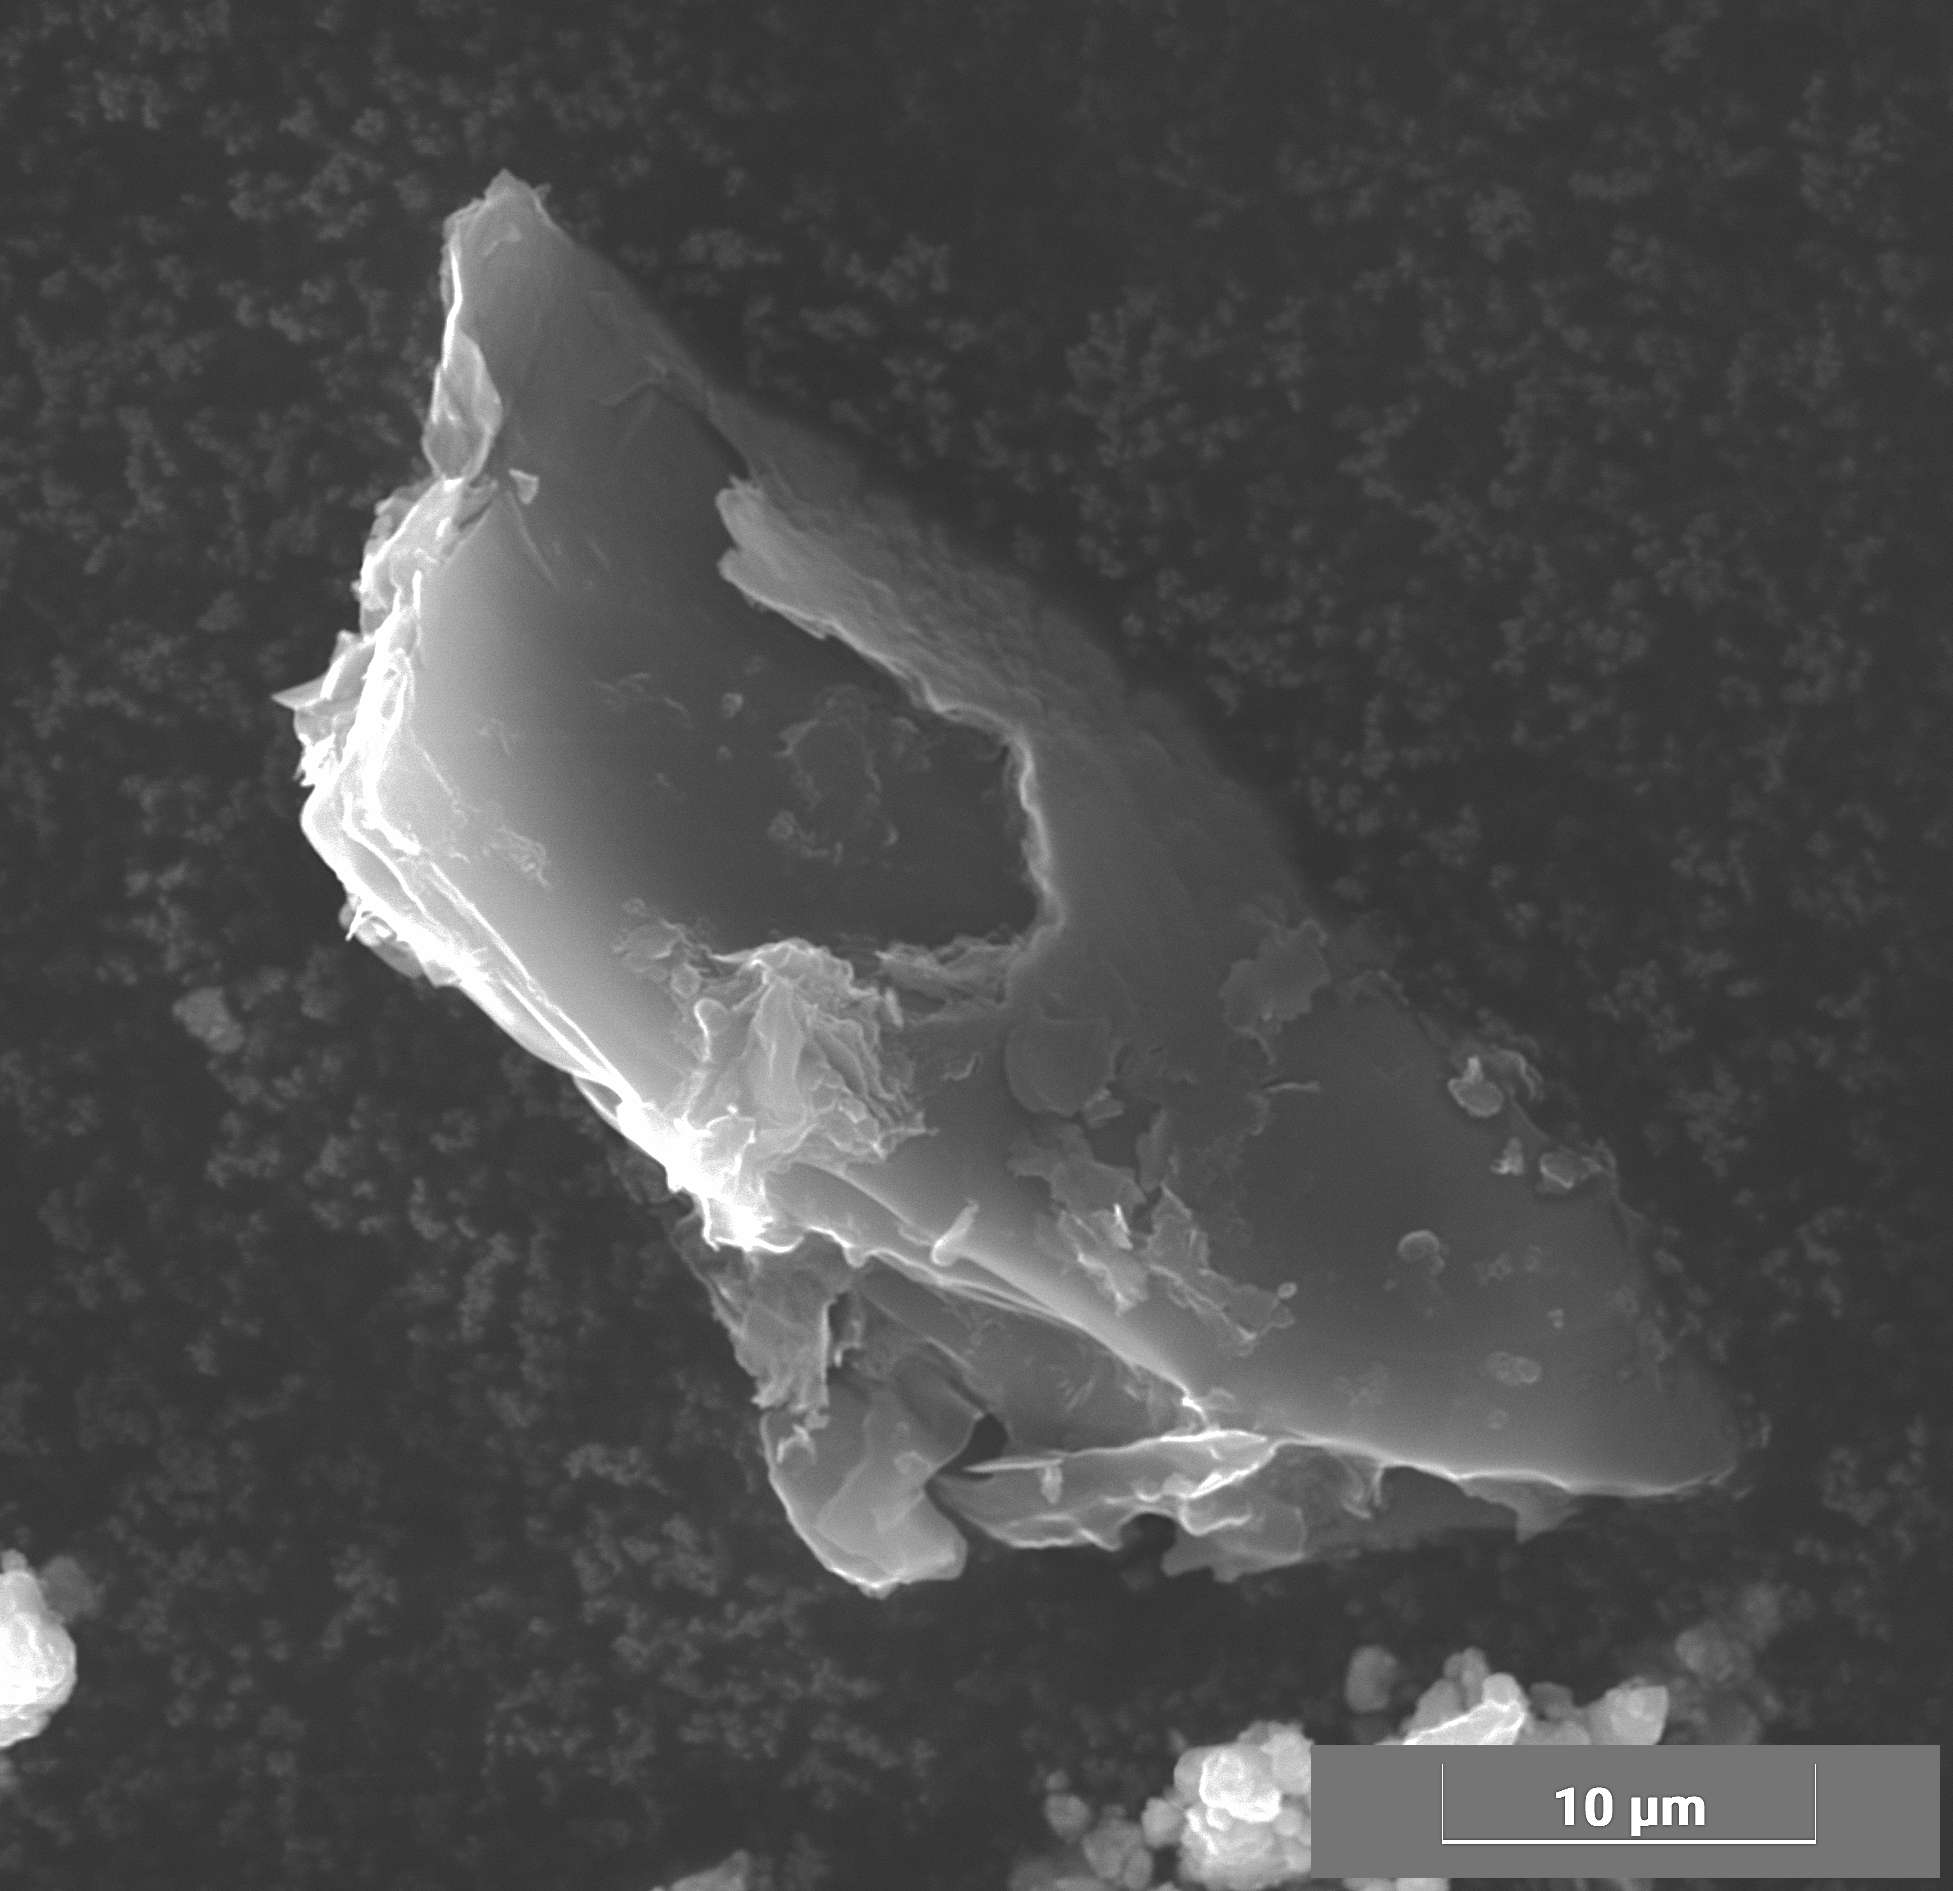
\includegraphics[width=\linewidth]{images/500L POST11 lamellar.png}
		\caption{500L Post}
		\label{fig:500L_Post_Lamellar}
	   \end{subfigure}
	   \begin{subfigure}{0.43\linewidth}
		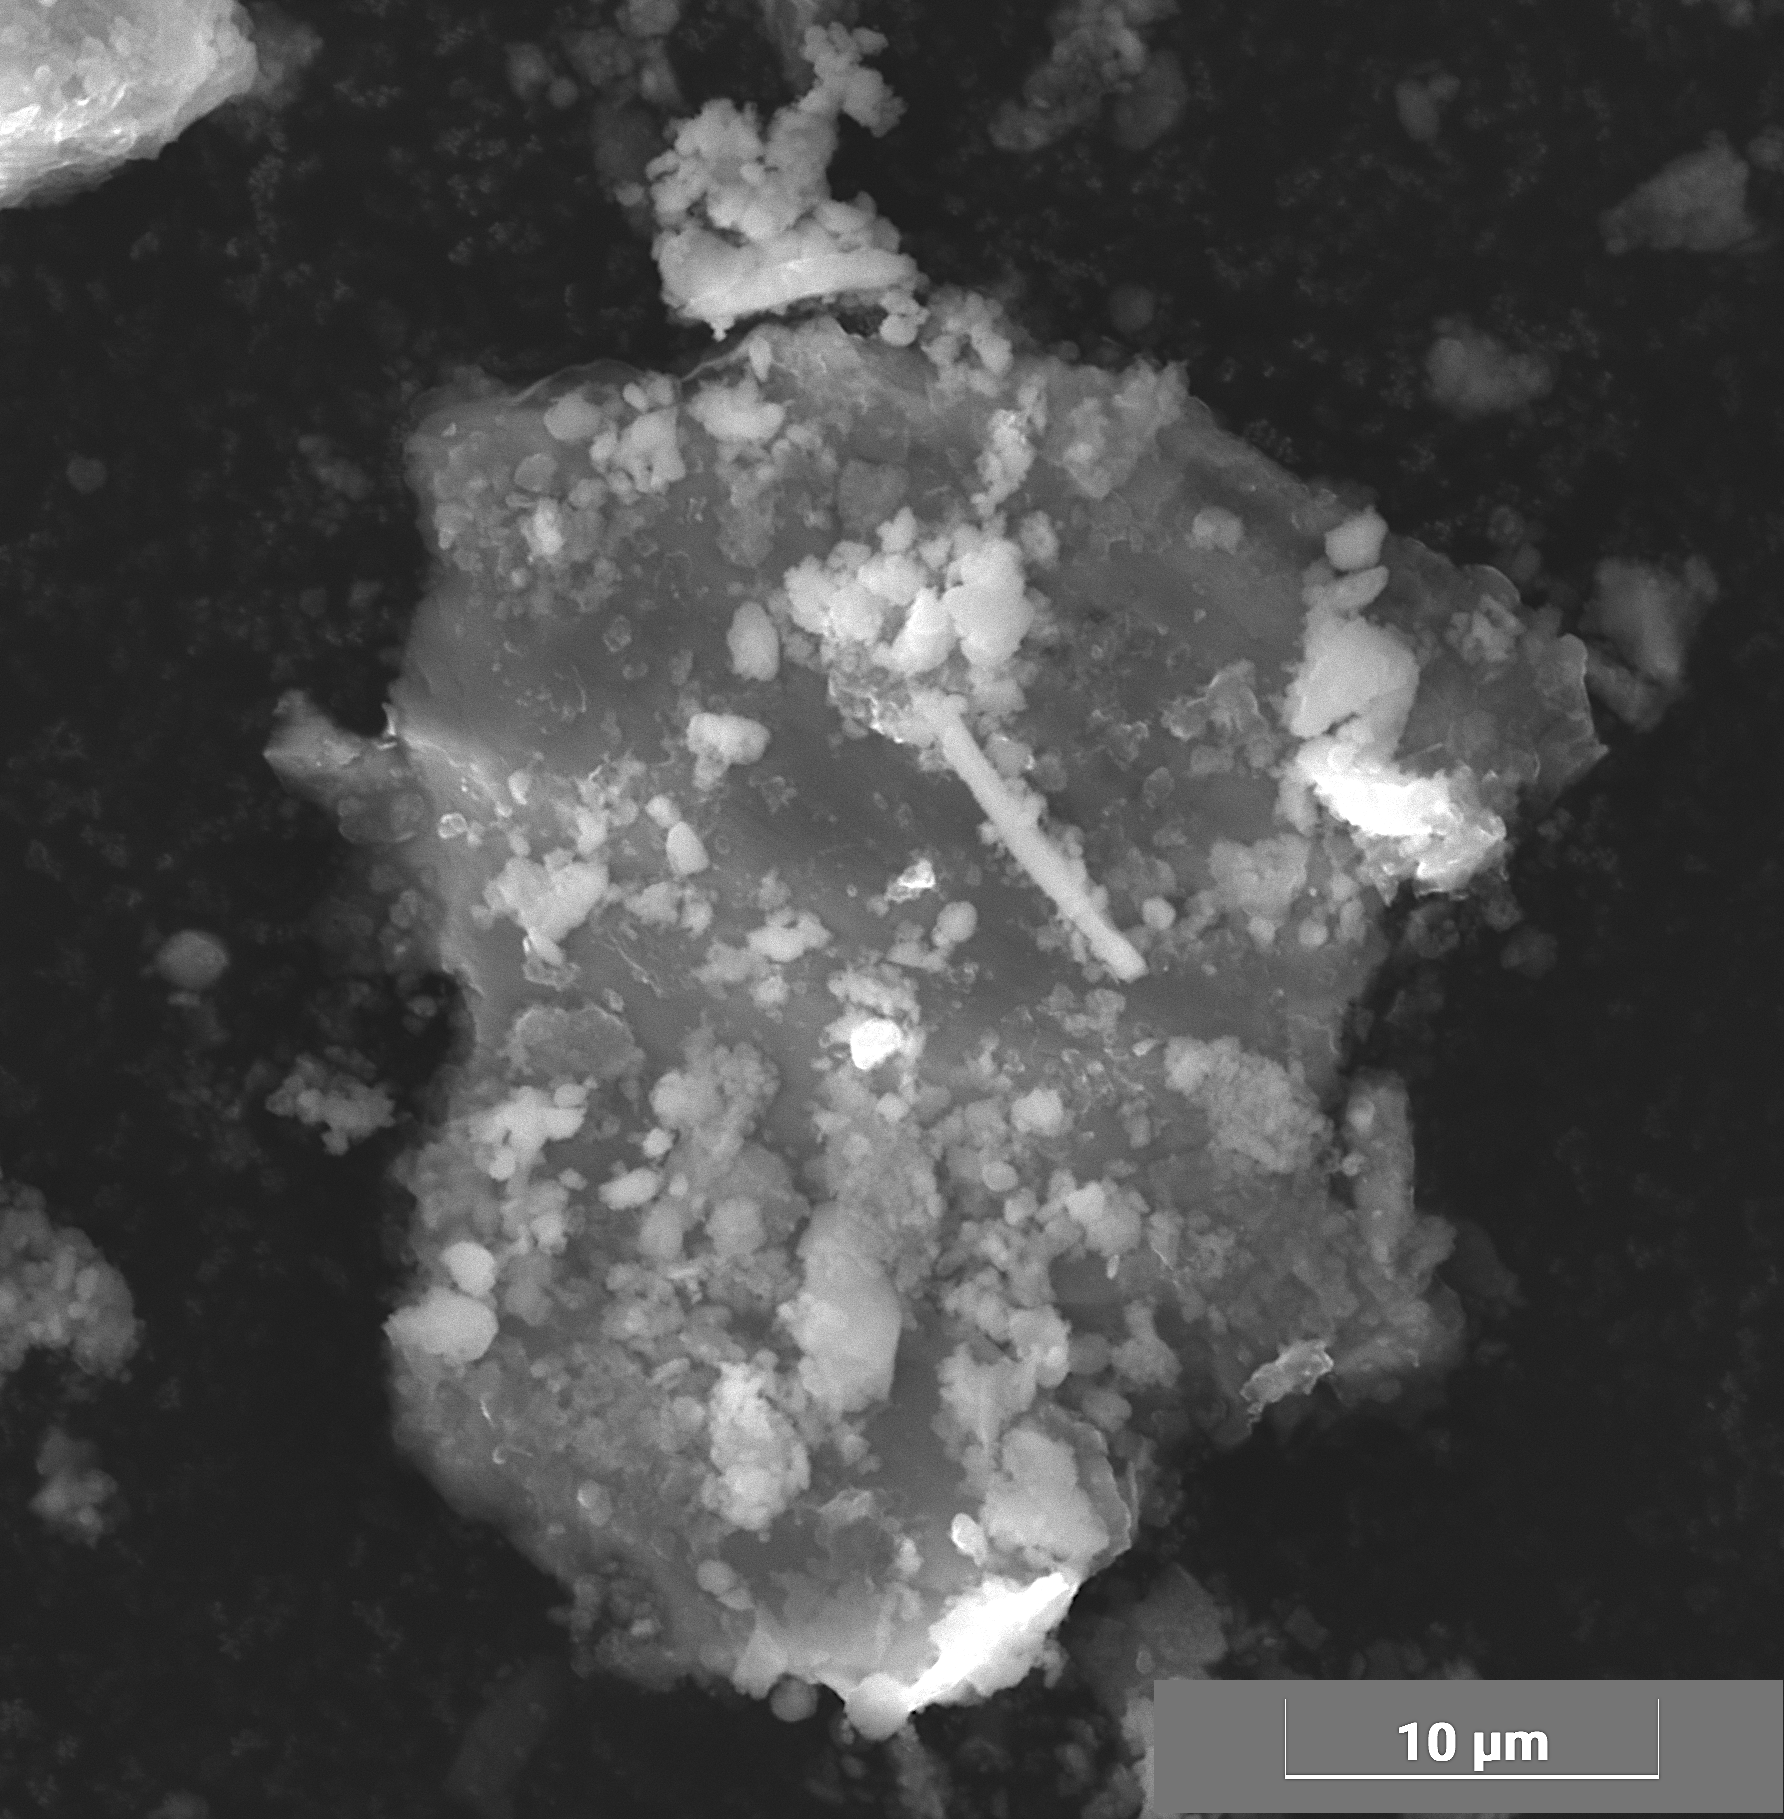
\includegraphics[width=\linewidth]{images/500X POST03 lamellar.png}
		\caption{500X Post}
		\label{fig:500X_Post_Lamellar}
	    \end{subfigure}
	\vfill
	     \begin{subfigure}{0.45\linewidth}
		 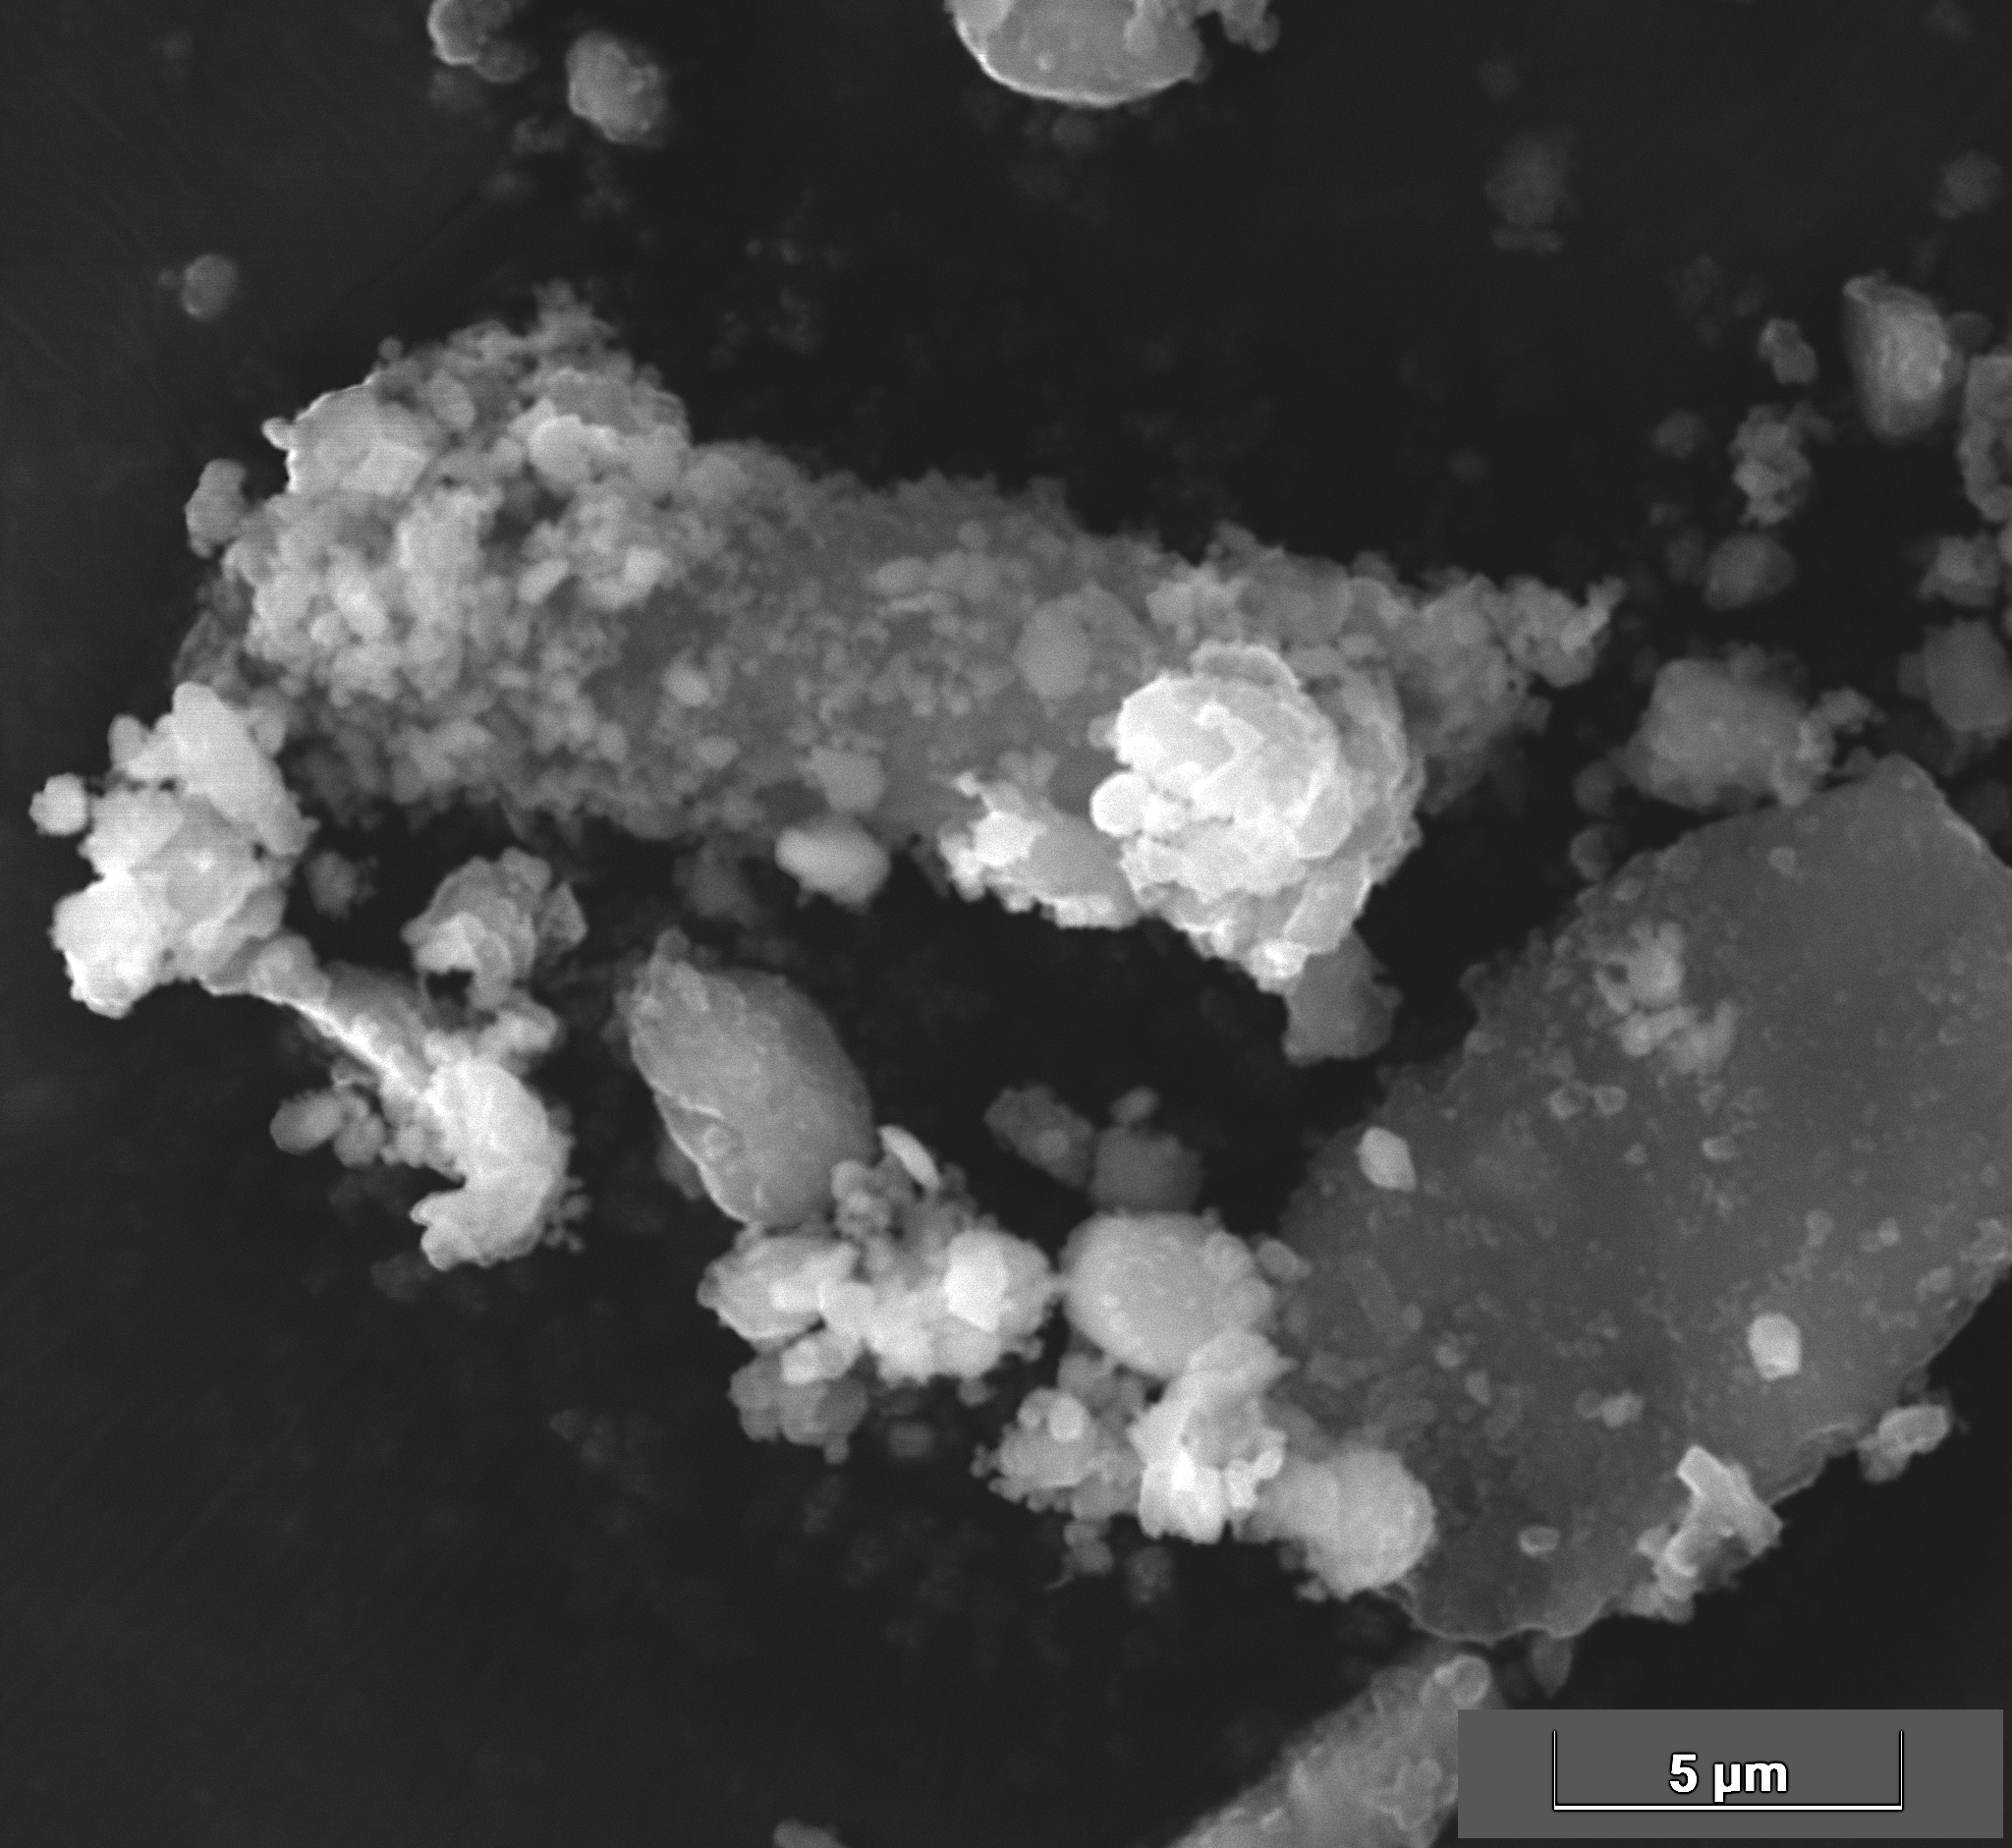
\includegraphics[width=\linewidth]{images/COROLLA ANT05 lamellar.png}
		 \caption{Corolla Ant}
		 \label{fig:Corolla_Ant_Lamellar}
	      \end{subfigure}
	       \begin{subfigure}{0.45\linewidth}
		  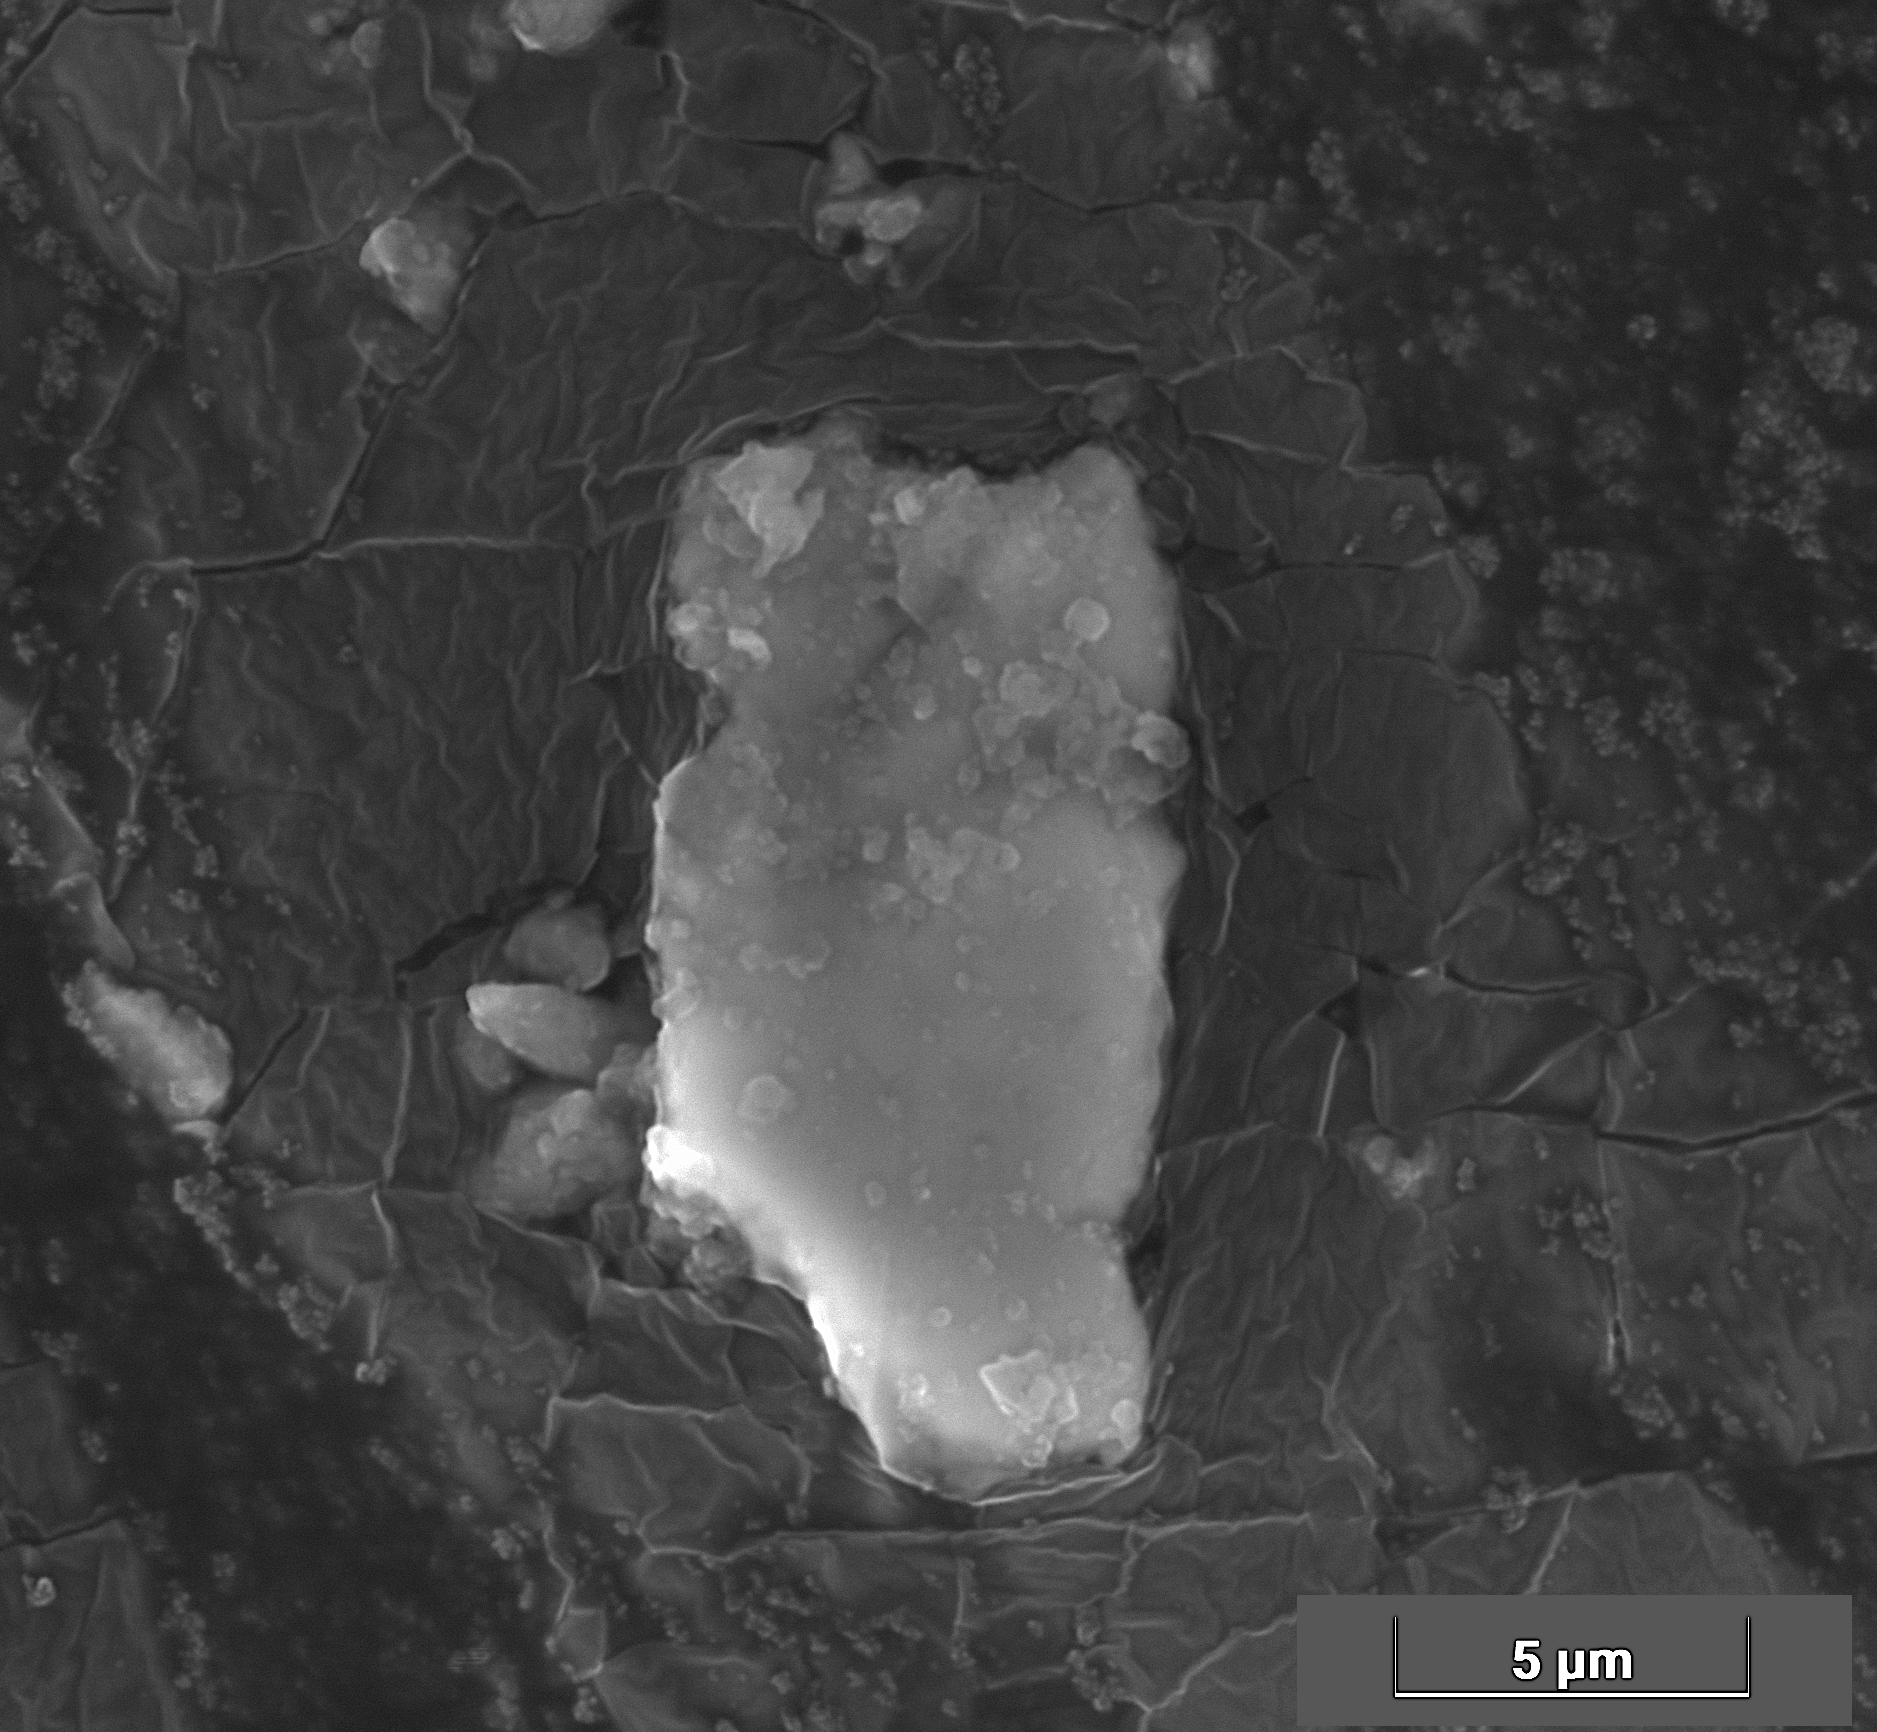
\includegraphics[width=\linewidth]{images/YPSILON POST10 lamellar.png}
		  \caption{Ypsilon Post}
		  \label{fig:Ypsilon_Post_Lamellar}
	       \end{subfigure}
\caption{Examples of lamellar shapes found in differnet samples. (a) a single lamellar particle. (b) lamellar particle with smaller ones on top. (c) on the right a lamellar particle. (d). single lamellar particle. }
	\label{fig:Lamellar}
\end{figure}




%Additionally, some particles exhibited striations, likely indicating sliding motions.
























\bibliographystyle{apalike}
\bibliography{Bibliography}
\afterpage{\blankpage}
\thispagestyle{plain}
\textbf{There will be the thanks to precious people here.}

\lipsum[1-3]

\end{document}
% -----------------------------------------------------------------
